\documentclass[jair,twoside,11pt,theapa]{article}
\usepackage{jair, theapa, rawfonts}
\usepackage[implicit=false]{hyperref}
\usepackage{amsmath,amsfonts, mathtools, bm}
\usepackage{xcolor}
\usepackage{colortbl}
\usepackage{algorithm}
\usepackage{algorithmic}
\usepackage{makecell}
\usepackage{tikz}
\usepackage{pifont}
\usepackage{pgfplots}
\usepackage{booktabs}
\pgfplotsset{compat=1.7}
\usepackage{bbm}
\usepackage{subcaption} % Add the subcaption package
\usetikzlibrary{arrows,matrix, positioning, shapes.geometric}
\usepackage{listofitems} 
\tikzstyle{mynode}=[thick,inner sep={.75\pgflinewidth}, draw=black,fill=white,circle,minimum size=3]
\jairheading{1}{2023}{1-15}{6/91}{9/91}
\ShortHeadings{Decision-Focused Learning: A Survey}{Mandi, Kotary, et al.}
\firstpageno{1}

\DeclareMathOperator*{\argmax}{argmax}
\DeclareMathOperator*{\argmin}{argmin}
\newcommand{\coloredasterisk}[1]{\textcolor{#1}{\ding{81}}}
\newcommand{\coloredx}[1]{\textcolor{#1}{\ding{54}}}
\newcommand{\coloredplus}[1]{\textcolor{#1}{\ding{58}}}
\newcommand{\coloredtriangle}[1]{\textcolor{#1}{\ding{115}}}
\newcommand{\coloredtriangledown}[1]{\textcolor{#1}{\ding{116}}}
\newcommand{\coloredtickmark}[1]{\textcolor{#1}{\ding{52}}}
\newcommand{\coloredcross}[1]{\textcolor{#1}{\ding{56}}}
\newcommand{\rev}[1]{{\color{purple}{#1}}}
\newcommand{\jk}[1]{{\color{blue}{#1}}}
\newcommand{\jay}[1]{{\color{blue}{jay: #1}}}
\newcommand{\senne}[1]{{\color{red}{Senne: #1}}}
\newcommand{\victor}[1]{{\color{brown}{Victor: #1}}}
\newcommand{\nando}[1]{{\color{purple}{\textbf{[}#1\textbf{]}}}}
\newcommand{\tias}[1]{{\color{teal}{Tias: #1}}}



\begin{document}

\title{Decision-Focused Learning: Foundations, State of the Art, Benchmark and Future Opportunities}

\author{\name Jayanta Mandi {\thanks{JM and JK should both be considered first authors.}} \email jayanta.mandi@vub.be \\
	\addr Vrije Universiteit Brussel,
	Belgium
	\AND
	\name James Kotary \email jkotary@syr.edu \\
	\addr Syracuse University, 
	USA
	\AND
	Senne Berden \email senne.berden@kuleuven.be \\
	\addr KU Leuven,
	Belgium
	\AND
	Maxime Mulamba \email maxime.mulamba@vub.be \\
	\addr Vrije Universiteit Brussel,
	Belgium
	\AND
	V\'ictor Bucarey \email victor.bucarey@uoh.cl \\
	\addr Universidad de O'Higgins,
	Chile
	\AND
	Tias Guns \email tias.guns@kuleuven.be \\
	\addr KU Leuven,
	Belgium
	\AND
	Ferdinando Fioretto \email fioretto@virginia.edu \\
	\addr University of Virginia,
	USA
	}


% For research notes, remove the comment character in the line below.
% \researchnote

\maketitle
\begin{abstract}
%In artificial intelligence (AI), operations research (OR) and business analytics (BA) decisions are often modeled using constrained optimization (CO) problems. However, real-world applications often require handling uncertainty or anticipating future events, rendering some parameters of the CO problems unknown during solving. When such parameters can be predicted as a function of observable features, predictions by conventional supervised learning often fall short in optimizing the resulting solutions. Decision-focused learning (DFL) is a paradigm that directly trains machine learning (ML) models to predict the unknown parameters in a way that leads to high-quality solutions. Since the loss function of the ML model becomes dependent on the solution of the CO problem, DFL entails an integration of its prediction and optimization components. As many ML models, including neural networks, are trained via gradient-based optimization, the challenge in this integration lies in backpropagation of gradients through the CO problem. This manuscript offers a comprehensive overview of methodologies developed for DFL, proposing a taxonomy to classify them based on their overall approach to backpropagating the gradients through the CO problem. Furthermore, the manuscript compares selected methodologies using publicly available benchmark datasets suitable for DFL and offers insights into current and future research directions in DFL. 
\emph{Decision-focused learning} (DFL) is an emerging paradigm in machine learning
which trains a model to optimize decisions, integrating prediction and optimization
in an end-to-end system. This paradigm holds the promise to revolutionize 
decision-making in many real-world applications which operate under uncertainty, 
where the estimation of unknown parameters within these decision models 
often becomes a substantial roadblock. 
This paper presents a comprehensive review of DFL. 
It provides an in-depth analysis of the various techniques devised
to integrate machine learning and optimization models, introduces 
a taxonomy of DFL methods distinguished by their unique characteristics, 
and conducts an extensive empirical evaluation of these methods proposing 
suitable benchmark dataset and tasks for DFL. 
Finally, the study provides valuable insights into current and potential 
future avenues in DFL research.
\end{abstract}


% \begin{keywords}
% 	predict-then-optimize, decision-focused learning, combinatorial optimization,  linear programming, stochastic optimization
% \end{keywords}

\section{Introduction}
% A large number of real-world applications deal with the challenge of decision making under uncertainty \cite{SAHINIDIS2004971,liu2009theory}.
% For example, a system that plans the shortest driving route between two locations in a city must first be able to infer the transit time associated with each city block \cite{kim2005optimal}. Likewise, the optimal power generation schedule in an electric grid can only be accurately modeled if future demands are known \cite{hu2016toward}. Furthermore, a common challenge in portfolio management involves optimizing total future returns subject to risk constraints, even before individual asset returns are known \cite{delage2010distributionally, 10.1093/rfs/hhl003}. 
% In numerous applications like these, the estimation of unknown parameters within a decision model often becomes a substantial obstacle. 

% In these contexts, Machine learning (ML) and Constrained Optimization (CO) emerge as two instrumental tools to addressing these intricate problems. 
% ML models estimate the uncertain quantities by leveraging correlated data, while CO models focus on optimizing objective functions within constrained spaces. This sequential process is commonly identified as the \emph{predictive} and \emph{prescriptive} aspects of analytical modeling in fields such as operations research and business analytics \cite{den2016bridging}, as illustrated in Figure~\ref{fig:problem_desc}. For example, in portfolio management, predictive modeling involves forecasting the returns of the assets, while prescriptive modeling is used to optimize total future returns based on these predictions.
Real-world applications frequently confront the task of decision-making under uncertainty, such as planning the shortest route in a city, determining optimal power generation schedules, or managing investment portfolios \cite{SAHINIDIS2004971,liu2009theory,kim2005optimal,hu2016toward,delage2010distributionally,hhl003}. In such scenarios, estimating unknown parameters often poses a significant challenge. 

Machine Learning (ML) and Constrained Optimization (CO) serve as two key tools for these complex problems. ML models estimate uncertain quantities, while CO models optimize objectives within constrained spaces. This sequential process, commonly referred to as \emph{predictive} and \emph{prescriptive} modeling, as illustrated in Figure~\ref{fig:problem_desc}, is prevalent in fields like operations research and business analytics \cite{den2016bridging}. For instance, in portfolio management, the prediction stage forecasts asset returns, while the prescriptive phase optimizes returns based on these predictions.

A commonly adopted approach involves handling these two stages---prediction and optimization---separately and independently. 
This ``two-stage'' process first involves training an ML model to create a mapping between observed features and the relevant parameters of a CO problem.
Subsequently, and independently, a specialized optimization algorithm is used to solve the decision problem, which is specified by the predicted problem parameters.
The underlying assumption in this methodology is that superior predictions would lead to precise models and consequently, high-quality decisions. Indeed, if the predictions of parameters were perfectly accurate, they would enable the correct specification of CO models which can be solved to yield fully optimal decisions.
However, ML models often fall short of perfect accuracy, leading to suboptimal decisions due to propagated prediction errors. Thus, in many applications, the predictive and prescriptive modelings are not isolated but rather, deeply interconnected, and hence should ideally be modeled jointly. 

% Figure environment removed

This is the goal of the \textbf{decision-focused learning} (DFL) paradigm, which directly trains the ML model to make predictions that lead to good decisions. In other words, DFL integrates prediction and optimization in an end-to-end system trained to optimize a criterion (i.e., a loss function) that is based on the resulting decisions.

Since many ML models, including neural networks (NNs), are trained via gradient-based optimization, the gradients of the loss must be backpropagated through each constituent operation of the model.  In DFL, the loss function is dependent on the solution of an optimization model, thus the optimization solver is \emph{embedded} as a component of the ML model. In this integration of prediction and optimization, a key challenge is \emph{differentiating through the optimization problem}. %viewed as a mapping from the predicted parameters to the resulting optimal solution. 
An additional challenge arises from decision models operating on discrete variables, which produce discontinuous mappings and hinder gradient-based learning. Hence, examining \emph{smooth} surrogate models for these discrete mappings, along with their differentiation, becomes crucial. These two challenges are the core emphasis and central focal points in DFL.
%a central focus of this survey.%, will be thoroughly explored, shedding light on and reviewing proposed solutions.


This manuscript presents a comprehensive survey of decision-focused learning and makes several contributions. First, to navigate the complex methodologies developed in recent years, the paper proposes the first categorization of DFL methods into four distinct classes: \textbf{(1)} analytical differentiation of optimization mappings, \textbf{(2)} analytical smoothing of optimization mappings, \textbf{(3)} smoothing by random perturbations,
and \textbf{(4)} differentiation of surrogate loss functions.
This categorization, as illustrated in Figure \ref{Fig:DFLMethodologyTable}, serves as a framework for comprehending and organizing various DFL methodologies.
Next, the paper compiles a selection of problem-specific DFL models, making them publicly available to facilitate broader access and usage.
An integral part of this paper involves benchmarking the performance of various available methodologies on \emph{seven} distinct problems. This provides an opportunity for comparative understanding and assists in identifying the relative strengths and weaknesses of each approach.
The code and data used in the benchmarking are accessible through \url{https://github.com/PredOpt/predopt-benchmarks}.
Finally, this survey addresses the critical need to look forward, by discussing the outstanding challenges and offering an outlook on potential future directions in the field of DFL. 

\subsection*{Paper organization.}
Following this introduction, the paper is structured as follows. Preliminary concepts are discussed in Section \ref{sect:prelim}, which introduces the problem setting and explicates the challenges in implementing DFL. The subsequent Section \ref{sect:review} offers a comprehensive review of recently proposed methodologies for handling these challenges, neatly organized into broad classes of related techniques. 
Secion \ref{sect:applications} presents interesting real-world examples of DFL applications.
Section \ref{sect:data} brings forth seven benchmark DFL tasks from public datasets, with a comparative evaluation of eight DFL methodologies presented in the following section. The manuscript concludes by providing a discourse on the current challenges and possible future directions in DFL research.


\section{Preliminaries}\label{sect:prelim}

This section presents an overview of the problem setting, along with preliminary concepts and essential terminology. Then, the central modeling challenges are discussed, setting the stage for a review of current methodologies in the design and implementation of DFL solutions.
Throughout the manuscript, vectors are denoted by boldface lowercase letters, such as $\mathbf{x}$, while scalar components within the vector $\mathbf{x}$ are represented with a subscript $i$, denoting the $i^{\text{th}}$ item within $\mathbf{x}$ as $x_i$. Similarly, the vectors $\mathbf{1}$ and $\mathbf{0}$ symbolize the vector of all-ones and all-zeros, respectively.

\subsection{Problem Setting}
\label{subsec:problem_description}


In operations research and business analytics, decisions are often quantitatively modeled using CO problems. 
These problems model various decision-making scenarios, but may not be efficiently solvable and often demand specialized solution algorithms that are tailored to their specific form.
In many real-world applications, some parameters of the CO problems are uncertain and must be inferred from contextual data (hereafter referred to as \emph{features}).
The settings considered in this manuscript involve estimating those parameters through predictive inferences made by ML models, and subsequently, the final decisions are modeled as the solution to the CO problems based on those inferences. 
% Figure \ref{fig:problem_desc} illustrates the sequential process of tackling such problems with \emph{predictive} and \emph{prescriptive} analytics. 

In this setting, the decision-making processes can be described by \emph{parametric} CO problems, defined as,
\begin{subequations}
\label{eq:opt_generic}
\begin{align}
    \label{eq:opt_generic_obj}
    \mathbf{x}^\star( \mathbf{c} ) = \argmin_{ \mathbf{x}} &\;\;
    f(\mathbf{x}, \mathbf{c})\\
    \label{eq:opt_generic_ineq}
    \texttt{s.t.} &\;\;
    \bm{g}( \mathbf{x}, \mathbf{c}) \leq \mathbf{0}\\
    \label{eq:opt_generic_eq}
    &\;\; \bm{h}(\mathbf{x}, \mathbf{c}) = \mathbf{0}.
\end{align}
\end{subequations}
The goal of the optimization problem above is to find \emph{a} solution $\mathbf{x}^\star(\mathbf{c}) \in \mathbb{R}^n$, a minimizer of the objective function $f$, satisfying a set $\bm{g}$ of inequality and a set $\bm{h}$ of equality constraints.
The \emph{parametric} problem formulation defines $\mathbf{x}^\star(\mathbf{c})$ as a function of the parameters $\mathbf{c} \in \mathbb{R}^k$. In the present setting, this function can naturally be interpreted as part of an overall composite function that encompasses ML inference and decision-making, and returns optimal decisions given feature variables as input. 
% In the context of DFL, we will later assume that $\mathbf{c}$ is a unknown parameter vector, which need to be predicted. 

CO problems can be categorized in terms of the forms taken by the functions defining their objectives (\ref{eq:opt_generic_obj}) and constraints (\ref{eq:opt_generic_ineq}-\ref{eq:opt_generic_eq}). These forms also determine important properties of the optimization mapping $\mathbf{c} \rightarrow \mathbf{x}^\star(\mathbf{c})$ when viewed as a function from problem parameters to optimal solutions, such as its continuity, differentiability, and injectivity.

In this manuscript, it is assumed that the constraints are fully known prior to solving, i.e., $\bm{h}(\mathbf{x},\mathbf{c}) = \bm{h}(\mathbf{x})$ and $\bm{g}( \mathbf{x},\mathbf{c}) = \bm{g}( \mathbf{x})$, and restrict the dependence on $\mathbf{c}$ to the objective function only. This is the setting considered by almost all existing works surveyed. While it is also possible to consider uncertainty in the constraints, this leads to the possibility of predicting parameters that lead to solutions that are infeasible with respect to the ground-truth parameters. The learning problem has not yet been well-defined in this setting (unless a recourse action to correct infeasible solutions is used \cite{PredictOptimizeforPacking,hu2023branch}). For this reason, in the following sections, only $f$ is assumed to depend on $\mathbf{c}$, so that $\bm{g}(\mathbf{x}) \leq \mathbf{0}$ and $\bm{h}(\mathbf{x}) = \mathbf{0}$ are satisfied for all outputs of the decision model. For notational convenience, the feasible region of the CO problem in \eqref{eq:opt_generic}, will be denoted by $\mathcal{F}$ (i.e., $\mathbf{x} \in \mathcal{F}$ if and only if $\bm{g}(\mathbf{x}) \leq \mathbf{0}$ and $\bm{h}(\mathbf{x}) = \mathbf{0}$).




If the true parameters $\mathbf{c}$ are known exactly, the corresponding `true' optimal decisions may be computed by solving \eqref{eq:opt_generic}. In such scenarios, $\mathbf{x}^\star (\mathbf{c})$ will referred to as the \emph{full-information optimal decisions} \cite{bertsimas2020predictive}. 
This paper, instead, considers problems where the parameters $\mathbf{c}$ are unknown but can be estimated as a function of empirically observed features $\mathbf{z}$. The problem of estimating $\mathbf{c}$ falls under the category of supervised machine learning problems. In this setting, a set of past observation pairs $\{ (\mathbf{z_i}, \mathbf{c_i})  \}_{i=1}^N$ is available and used to train a ML model $m_{\bm{\omega}}$ (with trainable parameters $\bm{\omega}$), so that parameter predictions take the form $\mathbf{\hat{ \mathbf{c}}} = m_{\bm{\omega}}( \mathbf{z})$. Then, a decision $\mathbf{x}^\star ( \mathbf{ \hat{c} })$ can be made based on the predicted parameters. $\mathbf{x}^\star ( \mathbf{ \hat{c} })$  is referred to as a \emph{prescriptive decision}. 
% The optimality of $\mathbf{x}^\star ( \mathbf{ \hat{c} })$  under ground-truth parameters $\mathbf{c}$ can subsequently be evaluated. 
The overall learning goal is to optimize the set of prescriptive decisions made over a distribution of feature variables $\mathbf{z} \sim \mathcal{Z}$, with respect to some evaluation criterion on those decisions. Thus, while the machine learning model $m_{\bm{\omega}}$ is trained to predict $\mathbf{\hat{c}}$, its performance is evaluated on the basis of the corresponding optimal solutions $\mathbf{x}^\star ( \mathbf{\hat{c}})$.
This paper uses the terminology \textit{Predict-Then-Optimize} problem to refer to the problem of predicting $\mathbf{\hat{c}}$, to improve the evaluation of $\mathbf{x}^\star ( \mathbf{\hat{c}})$. 

\subsection{Learning Paradigms}\label{sect:learningparadigm}
The defining challenge of the Predict-Then-Optimize problem setting is the gap in modeling between the prediction and the optimization components: while $m_{\bm{\omega}}$ is trained to predict $\mathbf{\hat{c}}$, it is evaluated based on the subsequently computed $\mathbf{x}^\star(\mathbf{\hat{c}})$. Using standard ML approaches,  learning of the predictions $\mathbf{\hat{c}} = m_{\bm{\omega}}(\mathbf{z})$ can only be supervised by the ground-truth $\mathbf{c}$ under standard loss functions $\mathcal{L}$, such as mean squared error or cross-entropy. In principle, it is favorable to  train $m_{\bm{\omega}}$ to make predictions $\mathbf{\hat{c}}$ that optimize the evaluation criterion on $\mathbf{x}^{\star}(\mathbf{\hat{c}})$ directly. This distinction motivates the definition of two alternative learning paradigms for Predict-Then-Optimize problems.   

\paragraph{Prediction-focused learning (PFL).}  A straightforward approach to this supervised ML problem is to train the model to generate accurate  parameter predictions $\mathbf{\hat{c}}$ with respect to ground-truth values $\mathbf{c}$.
This paper introduces the term \emph{prediction-focused learning} to refer to this approach (also called two-stage learning \cite{aaai/WilderDT19}) because the model is trained with a focus on the accuracy of the parameter predictions preceding the decision model. Here, the training is agnostic of the downstream optimization problem. At the time of making the decision, the pre-trained model's predictions $\mathbf{\hat{c}}$ are passed to optimization routines which solve \eqref{eq:opt_generic} to return $\mathbf{x}^\star (\mathbf{\hat{c}})$. Typical ML losses, such as the mean squared error (MSE) or binary cross entropy (BCE), are used to train the prediction model in this case.
\iffalse
\begin{equation}
    MSE(\mathbf{\mathbf{\hat{c}}}, \mathbf{c}) = \frac{1}{N} \sum_{i=1}^N \bigg( c_i - \mathbf{\hat{c}}_i \bigg)^2
    \label{eq:prediction_focused}
\end{equation}
\fi
\begin{equation}
    MSE(\mathbf{\hat{c}}, \mathbf{c}) = \frac{1}{N} \| \mathbf{c} - \mathbf{\hat{c}} \| ^2
    \label{eq:prediction_focused}
\end{equation}
\noindent 
Such loss functions, like Eq. \eqref{eq:prediction_focused}, which measure the prediction error of $\mathbf{\hat{c}}$ with respect to $\mathbf{c}$, are referred to as \textit{prediction losses}.
Algorithm ~\ref{alg:prediction_focused} illustrates prediction-focused learning using the MSE loss. 


\iffalse
\rev{JK: Architectures don't train the models. This sentence is floating by itself so I removed it.}
Modern deep learning architectures train the ML models by stochastic gradient-descent (SGD), where $\omega$ is iteratively updated in the opposite direction of the gradient of the loss function with respect to $\omega$.
\fi
\paragraph{Decision-focused learning (DFL).} 
By contrast, in \textit{decision-focused} learning, the ML model is trained to optimize the evaluation criteria which measure the quality of the resulting decisions. As the decisions are realized after the optimization stage, this requires the integration of prediction and optimization components, into a composite model which produces full decisions. From this point of view, generating the predicted parameters $\mathbf{\hat{c}}$ is an intermediary step of the integrated approach, and the accuracy of $\mathbf{\hat{c}}$ is not the primary focus in training. The focus, rather, is on the error incurred after optimization. A measure of error with respect to the integrated model's prescriptive decisions, when used as a loss function for training, is henceforth referred to as a \textit{task loss}. The essential difference from the aforementioned prediction loss is that it measures the error in $\mathbf{x}^{\star}(\mathbf{\hat{c}})$, rather than in $\mathbf{\hat{c}}$.

The objective value achieved by using the predicted $\mathbf{x}^\star (\mathbf{\hat{c}})$ is generally suboptimal
 with respect to the true objective parameters $\mathbf{c}$. Often, the end goal is to generate predictions $\mathbf{\hat{c}}$ with an optimal solution $\mathbf{x}^\star (\mathbf{\hat{c}})$ whose objective value in practice (i.e., $f(\mathbf{x}^\star(\mathbf{\hat{c}}),\mathbf{ c})$) comes close to the full-information optimal value $f(\mathbf{x}^\star( \mathbf{c}), \mathbf{c})$. In such cases, a salient notion of task loss is the \emph{regret}, defined as  the difference between the full-information optimal objective value and the objective value realized by the prescriptive decision. Equivalently, it is the magnitude of suboptimality of the decision $\mathbf{x}^\star(\mathbf{\hat{c}})$ with respect to the optimal solution $\mathbf{x}^\star( \mathbf{c})$ under ground-truth parameters $\mathbf{c}$:
\begin{equation}
\textit{Regret}(\mathbf{x}^\star(\mathbf{\hat{c}}),\mathbf{ c })= f(\mathbf{x}^\star (\mathbf{\hat{c}}), \mathbf{c}) - f(\mathbf{x}^\star( \mathbf{c}), \mathbf{c})
\label{eq:regret}
\end{equation}
\iffalse
% Figure environment removed
\fi
\noindent
Note that minimizing regret is equivalent to minimizing the value of $f(\mathbf{x}^\star (\mathbf{\hat{c}}), \mathbf{c})$, since the term $f(\mathbf{x}^\star( \mathbf{c}), \mathbf{c})$ is constant with respect to the prediction model.  While regret may be considered the quintessential example of a task loss, other task losses can arise in practice. For example, when the ground-truth target data are observed in terms of decision values $\mathbf{x}$, rather than parameter values $\mathbf{c}$, they may be targeted using the typical training loss functions such as $MSE(\mathbf{x}^{\star}(\mathbf{\hat{c}}), \mathbf{x})$. 

\iffalse
\jay{Q to others: Would it be fine to put the following text here, or remove because it breaks the flow:
Note that in some optimization problems, the predicted cost vector $\mathbf{ \hat{c} }$ might have multiple non-unique optimal solutions.  
In such cases, \citeA{elmachtoub2022smart} propose to consider the worst-case regret.
To do so, the set of optimal solutions of $\mathbf{ \hat{c} }$ can be represented by $\mathcal{X} ^\star ( \hat{c} )$.
And then the worst-case regret can be defined in the following form:
\begin{equation}
    \textit{Regret}(\mathbf{x}^\star(\hat{c}),c )= \max_{\mathbf{x}^\star ( \mathbf{ \hat{c}} ) \in \mathcal{X} ^\star ( \hat{c} )} f(\mathbf{x}^\star ( \mathbf{ \hat{c}} ), c) - f(\mathbf{x}^\star( c), c)
    \label{eq:worstregret_lp}
\end{equation}
}
\senne{I am still of the opinion that it would break the flow and does not belong in this part of the text.}\tias{I agree, it is too far from practice. It would fit in a discussion session, that there might be equivalent solutions...}
\nando{Nando: Agreed.}

Note that in practice the mapping $c \rightarrow \mathbf{x}^\star (\mathbf{c})$ can be one-to-many, meaning that there are non-unique solutions of $\mathbf{c}$. 
In this case, the set of optimal solutions of $\mathbf{c}$ can be represented by $\mathcal{X} ^\star ( \mathbf{c}) = \argmin \{ c^\top x| Ax=b; x\geq 0 \} $.
In case $\mathbf{ \hat{c} }$ has non-unique solutions, the value of the regret would change based on which $\mathbf{x}^\star ( \mathbf{ \hat{c}} ) \in \mathcal{X} ^\star ( \hat{c} )$ is considered in the regret computation. 
To address this, \citeA{elmachtoub2022smart} propose to consider the worst-case regret. \senne{Either remove this (since it's not a problem that ever occurs in practice), or add an explanation of why this never occurs.}
\begin{equation}
    \textit{Regret}(\mathbf{x}^\star(\hat{c}),c )= \max_{\mathbf{x}^\star ( \mathbf{ \hat{c}} ) \in \mathcal{X} ^\star ( \hat{c} )} c^\top ( \mathbf{x}^\star ( \hat{c}) - \mathbf{x}^\star ( \mathbf{c}))
    \label{eq:worstregret_lp}
\end{equation}
However, to avoid this complexity in our experiments, we assume that the solution $\mathbf{x}^\star(\mathbf{\hat{c}})$ is obtained by calling an optimization oracle and that if there exist non-unique solutions, the oracle simply returns a single optimal solution by breaking ties in a pre-specified manner.
\fi
\raggedbottom
 \paragraph{Relationship between prediction and task losses.} As previously mentioned, an ML model is trained without considering the downstream CO problem in prediction-focused learning for Predict-Then-Optimize tasks; still the ML model is evaluated at test time on the basis of its resulting CO problem solutions.
This is based on an underlying assumption that generating accurate predictions with respect to a standard prediction loss will result in good prescriptive decisions. Note that zero prediction loss always implies zero task loss, since $\mathbf{\hat{c}} = \mathbf{c}$ implies $\mathbf{x}^{\star}(\mathbf{\hat{c}}) = \mathbf{x}^{\star}(\mathbf{c})$. However, in practice, it is impossible to learn a model that makes no prediction error on any sample. 
The model error can only be minimized in one metric, and the minimization of the prediction error and the resulting decision error do not in general coincide \cite{aaai/WilderDT19}. 
Furthermore, the prediction loss and the task loss are, in general, not  continuously related. These principles are illustrated by the following example:
\paragraph{Example.}  The shortcomings of training with respect to prediction errors can be illustrated with a relatively simple CO problem. For this illustration, consider a knapsack problem \cite{pisinger1998knapsack}. 
The objective of the knapsack problem is to select a subset of maximal value  from an overall  set of items, each having its own value and unit weight, subject to a capacity constraint.
The capacity constraint imposes that the sum of the weights of the selected items cannot be higher than the capacity $C$. 
This knapsack problem with unit weights can be formulated as follows:
\begin{equation}
    \label{eq:unitknapsackformulation}
   \mathbf{x}^{\star}(\mathbf{c}) = \argmax_{\mathbf{x} \in \{0,1\} } \mathbf{c}^\top \mathbf{x} \;\; \texttt{s.t.} \sum_i x_i \leq \text{Capacity}
\end{equation}

In a Predict-Then-Optimize variant of this knapsack problem, the item weights and knapsack capacity are known, but the item values are unknown and must be predicted using observed features.
The ground-truth item value $\mathbf{c}$ implies the ground-truth solution $\mathbf{x}^\star (\mathbf{c})$. Overestimating the values of the items that are chosen in $\mathbf{x}^\star (\mathbf{c})$ (or underestimating the values of the items that are not chosen) increases the prediction error. Note that these kind of prediction errors, even if they are high,  
do not affect the solution, and thus do not affect the task loss either.  On the other hand, even low prediction errors for some item values may change the solution, affecting the task loss. That is why after a certain point, reducing prediction errors does not decrease task loss, and sometimes may increase it. DFL aims to address this shortcoming of PFL: by minimizing the task loss directly, prediction errors are implicitly traded off on the basis of how they affect the resulting decision errors. 


% Figure environment removed

% \jay{Q to others: Is the description of the numerical experiment too long, or is it better to keep the describe only in the caption }
% \senne{In my opinion it is fine to have this description here}

The discrepancy between the prediction loss and the task loss has been exemplified in Figure \ref{fig:knapsack_example} for a very simple knapsack problem with only two items. For this illustration, assume that both the items are of unit weights and the capacity of the knapsack is one, i.e., only one of the two items can be selected.
 The true values of the first and second items are $2.5$ and $3$ respectively. The point $(2.5,3)$, marked with \coloredasterisk{blue}, represents the true item values.
In this case the true solution is $(0,1)$, which corresponds to selecting only the second item. It is evident that any prediction in the blue shaded region leads to this solution. 
For instance, the point $(1.5,3)$, marked with \coloredplus{teal}, corresponds to predicting $1.5$ and $3$ as values of the two items respectively and this results in selecting the second item.
On the other hand, the point $(2.5,2)$, marked with \coloredx{magenta}, triggers the wrong solution $(1,0)$, although the squared error values of \coloredplus{teal} and \coloredx{magenta} are identical. 
Also, note that overestimating the value of the second item does not change the solution. For instance, the point $(1.5,4)$, marked with \coloredtriangle{teal}, corresponds to overestimating the value of the second item to $4$ while keeping the value of the first item the same as the point in \coloredplus{teal}.
 This point is positioned directly above the point in \coloredplus{teal} and still stays in the blue-shaded region.
 Similarly, the point $(0.5,3)$, marked with \coloredtriangledown{teal}, results from underestimating the value of the first item and is in the blue shaded region too. 
% On the other hand, the values of squared errors of the two points marked with \coloredtriangle{black} are $4.25= ( (2.5-2)^2 + (3-5)^2)$ and $4= ( (2.5-0.5)^2 + (3-3)^2)$ respectively.
 Although these two points have higher values of squared error than the point marked with \coloredx{magenta}, they trigger the right solution, resulting in zero regret. 
 
%%\textit{Decision-focused learning methods try to use the limited capacity of the predictive model and the finite availability of training data in a way thatspecifically avoids making prediction errors that negatively impact the quality of the resulting decisions.}


\iffalse
As an extreme example, consider the weighted knapsack problem \cite{pisinger1998knapsack}, and the task of predicting the values \cite{mandi2020smart} of each item. If the weight of some item is greater than the capacity of the knapsack, that item would not feature in the solution, regardless of its predicted value. Therefore while the error in that item's predicted value can be minimized with respect to the ground truth, it does not impact the resulting decision or its error.
\senne{This is true but feels like a trivial case since the weight of the item exceeds the capacity and so the prediction of that item's value never matters. I don't think that this would really convince the reader that the mapping between prediction and decision errors can be really complex. They might think: this is not convincing since the item for which the prediction is made is not really involved in the optimization. I will propose an alternative and then we can discuss. UPDATE: I have proposed an alternative; see below.}  \rev{JK: I think it is a decent example, because it illustrates how the change in solution wrt c is often discrete. Trivial but sufficient to prove the point. I gave a better explanation along with it. Check my revision above pls.} \senne{The change in solution with respect to c being discrete is relevant when talking about the uninformative gradients issue, but I don't think that it is that relevant when talking about why minimizing prediction error is not equivalent to minimizing task loss. After all, if the mapping from prediction error to task loss where non-strictly monotonically decreasing, then minimizing prediction error and minimizing task loss would be equivalent, even though the change in solution with respect to c is discrete.}

\senne{
UPDATE: here is my proposed alternative example. As an example, consider a weighted knapsack problem in which the item weights are given, but the item values are unknown and must be predicted from features. Ground-truth item values $\mathbf{c}$ invoke a ground-truth solution $\mathbf{x}^\star{c}$, which consists simply of $x_i = 1$ when $c_i$ one of the top $C$ item values. Relative to the ground-truth data, overestimating the values of the items that are chosen in $\mathbf{x}^\star{c}$ (or underestimating the values of the items that are not chosen) increases the prediction error $\|\hat{c} - c\|$, but does not affect the resulting presciptive decision, and thus does not affect the task loss either. 
}
\senne{Possible addition: Since any ML model has a limited representational capacity, allowing for these kinds of prediction errors to happen can enable the model to avoid prediction errors that actually do increase the task loss in a significant way. This is exactly what training the model using a task loss entails: prediction errors are implicitly traded off on the basis of how they affect the resulting decision error.}

\victor{I agree that James' example is too trivial, but it is self-explanatory. Senne's example is correct but it shows a pain where it does not hurt: If we increase the prediction error and do not change the decision error is not a problem by itself. We should state an example when you minimize the prediction error and at the same time you increase the decision error. Here we can show 2 things: 1. The example in the SPO paper (section 3.1); 2. the typical plot showing that decreasing MSE could increase the regret. 

In summary, I would write the following story: I wpould start with Jame's example. Then, I would comment Senne's example, and finally, I would mention the example that really hurts.  }
\fi





\paragraph{Empirical risk minimization and bilevel form of DFL.} The minimization of either the prediction loss in PFL or the task loss in DFL, can be expressed as an \emph{empirical risk minimization} (ERM) \cite{Vapnik99} problem over a training dataset containing feature variables and their corresponding parameters $\mathcal{D} \equiv \{(\mathbf{z_i}, \mathbf{c_i})\}_{i=1}^N$. For concreteness, the respective ERM problems below assume the use of the MSE and regret loss functions, but the principles described here hold for a wide range of alternative loss functions. 

PFL, by minimizing the prediction error with respect to the ground-truth parameters directly, takes the form of a standard regression problem:
\begin{equation}
    \min_{\bm{\omega}} \frac{1}{N} \sum_{i=1}^N \| m_{\bm{\omega}} (\mathbf{z_i})  - \mathbf{c_i} \|^2 \label{eq:ERM_PFL_outer},\\
\end{equation}
which is an instance of unconstrained optimization. In the case of DFL, it is natural to view the ERM as a bilevel optimization problem: 
%prediction and optimization steps the introduction of the optimization mapping $\mathbf{c} \to \mathbf{x}^{\star}(\mathbf{c})$
% use subequations to fix the eqn ref?
\begin{subequations}
\label{eq:bilevel}
\begin{align}
    \min_{\bm{\omega}} \frac{1}{N} \sum_{i=1}^N \Big( f(\mathbf{x}^\star(\mathbf{\hat{c}_i}), \mathbf{c_i}) - f(  \mathbf{x}^\star(\mathbf{c_i}), \mathbf{c_i}) \Big) \label{eq:bilevel_outer}\\
    \texttt{s.t.} \;\; \mathbf{\hat{c}_i} = m_{\bm{\omega} }(\mathbf{z_i})  ;\ \mathbf{\mathbf{x}^\star}(\mathbf{ \hat{c}_i }) = \argmin_{ \mathbf{x} \in \mathcal{F}} \mathbf{\hat{c}_i}^\top \mathbf{x} . \label{eq:bilevel_inner}
\end{align}
\end{subequations}
The outer-level problem \eqref{eq:bilevel_outer} minimizes task loss on the training set while the inner-level problem \eqref{eq:bilevel_inner} computes the mapping $\mathbf{c} \to \mathbf{x}^{\star}(\mathbf{c})$. 
Solving \eqref{eq:bilevel} is computationally more challenging than solving \eqref{eq:ERM_PFL_outer} in the prediction-focused paradigm. In both cases, optimization by stochastic gradient descent (SGD) is the preferred solution method for training neural networks.  

Algorithms ~\ref{alg:prediction_focused} and ~\ref{alg:decision_focused} compare the gradient descent training schemes for each of these problems. Algorithm ~\ref{alg:prediction_focused} is a standard application of gradient descent, in which the derivatives of Line \rev{6} are generally well-defined and can be computed straightforwardly (typically by automatic differentiation).
Line \rev{7} of Algorithm ~\ref{alg:decision_focused} shows that direct differentiation of the mapping $\mathbf{c} \to \mathbf{x}^{\star}(\mathbf{c})$ can be used to form the overall task loss gradient $\frac{d  \mathcal{L}} {d  \bm{\omega}}$,  by providing the required chain rule term $\frac{d  \mathbf{x}^\star( \mathbf{\hat{c}} )}{d  \mathbf{\hat{c}}}$. However, this differentiation is nontrivial as the mapping itself lacks a closed-form representation. Further, many interesting and practical optimization problems are inherently nondifferentiable and even discontinuous as functions of their parameters, precluding the direct application of Algorithm ~\ref{alg:decision_focused} to optimize ~\eqref{eq:bilevel} by gradient descent. The following subsections review the main challenges of implementing Algorithm ~\ref{alg:decision_focused}. 

\begin{minipage}[t]{0.4\textwidth}
    \begin{algorithm}[H]
\caption{Gradient-descent in prediction-focused learning}
\label{alg:prediction_focused}
\textbf{Input}: training data D$ \equiv \{(\mathbf{z_i},\mathbf{c_i})\}_{i=1}^N$ \\
\textbf{Hyperparams}: $\alpha$- learning rate\\
%\textbf{Output}: Your algorithm's output
\begin{algorithmic}[1] %[1] enables line numbers
\STATE Initialize $\bm{\omega}$.
\FOR{each epoch}
\FOR{each instance $(\mathbf{z},\mathbf{c})$}
\STATE $\mathbf{\hat{c}} = m_{\mathbf{\bm{\omega}}} ( \mathbf{z})$ \label{alg:ln:pred} %\# transform predictions.
\STATE $\mathcal{L} = (\mathbf{\hat{c}} -\mathbf{ c})^2$ \\
\STATE $\bm{\omega} \leftarrow \bm{\omega} - \alpha \frac{d  \mathcal{L}}{d  \mathbf{\hat{c}}} \frac{d  \mathbf{\hat{c}}}{d  \bm{\omega}}$

% \STATE $\bm{\omega} \leftarrow \bm{\omega} - \alpha \frac{d  L^{v}}{d  \tilde{c}} \frac{ d  \tilde{c}}{d  \bm{\omega}}$ \# backpropagate (sub)gradient
\ENDFOR
\ENDFOR
\end{algorithmic}
\end{algorithm}
\end{minipage}
\hspace{3mm}
\begin{minipage}[t]{0.55\textwidth}

\begin{algorithm}[H]
\caption{Gradient-descent in decision-focused learning with regret as task loss}
\label{alg:decision_focused}
\textbf{Input}: $\mathcal{F}$, training data D $\equiv \{(\mathbf{z_i}, \mathbf{c_i}, \mathbf{x}^\star(\mathbf{c_i})\}_{i=1}^N$; \\
\textbf{Hyperparams}: $\alpha$- learning rate\\
%\textbf{Output}: Your algorithm's output
\begin{algorithmic}[1] %[1] enables line numbers
\STATE Initialize $\bm{\omega}$.
\FOR{each epoch}
\FOR{each instance $(\mathbf{z},\mathbf{c}, \mathbf{x}^\star(\mathbf{c}))$}
\STATE $\mathbf{\hat{c}} = m_{\mathbf{\bm{\omega}}} (\mathbf{ z})$ \\
\STATE $\mathbf{x}^\star(\mathbf{\hat{c}} ) = \argmin_{\mathbf{x} \in \mathcal{F} } f( \mathbf{x}, \mathbf{\hat{c}})$ \\
%\# transform predictions.
\STATE $\mathcal{L} = f(\mathbf{x}^\star(\mathbf{\hat{c}}), \mathbf{c}) - f(\mathbf{x}^\star (\mathbf{c}), \mathbf{c})$ \\
\STATE $\bm{\omega} \leftarrow \bm{\omega} - \alpha \frac{d  \mathcal{L}}{d  \mathbf{x}^\star(\mathbf{\hat{c}} )}   \frac{d  \mathbf{x}^\star(\mathbf{\hat{c}} )}{d \mathbf{ \hat{c}}} \frac{d  \mathbf{\hat{c}}}{d  \bm{\omega}}$

% \STATE $\bm{\omega} \leftarrow \bm{\omega} - \alpha \frac{d  L^{v}}{d  \tilde{c}} \frac{ d  \tilde{c}}{d  \bm{\omega}}$ \# backpropagate (sub)gradient
\ENDFOR
\ENDFOR
\end{algorithmic}
\end{algorithm}
\end{minipage}






\iffalse
Formally we define an ILP as an optimization problem of the following form
\begin{align}
    & \min_{x \geq 0} c^\top x \nonumber \\
    & \text{such that } Ax = b; x \in \mathbb{Z}_{+}^n
    \label{eq:ILP}
\end{align}
\fi


\iffalse
We will use $\mathbf{x}^\star (\mathbf{c})$ to denote a solution of \eqref{eq:LP} or \eqref{eq:ILP}. \jay{So, we can view the LP or ILP as a mapping from $\mathbf{c}$ to $\mathbf{x}^\star (\mathbf{c})$.} [We note that there might be non-unique solutions, but we consider the optimization solver as an oracle which returns \emph{a} solution.] We may consider the optimization problem as a mapping from the coefficient vector $\mathbf{c}$ to its optimal solution(s).
\fi
% We remark that some of the literature, reviewed in this manuscript, may consider a more generic optimization form, such as 
% \begin{align}
%     & \min_{x  } f(c,x) \nonumber \\
%     & \text{such that } \bm{g}(x) \leq 0; \bm{h}(x)=0
%     \label{eq:generic_opt}
% \end{align}
% But our discussion and experimental evaluations are limited to optimization problems with linear objective function. 



\subsection{Challenges to Implement DFL}
\label{sect:challenge}
\paragraph{Differentiation of CO mappings.} To minimize a task loss by gradient descent training,  its partial derivatives with respect to the prediction model parameters $\bm{\omega}$ must be computed to carry out at the parameter update at Line \rev{7} of Algorithm \ref{alg:decision_focused}. Since the task loss $\mathcal{L}$ is a function of $\mathbf{x}^\star ( \mathbf{ \hat{c}} )$, the gradient of $\mathcal{L}$ with respect to $\bm{\omega}$ can be expressed in the following terms by using the chain rule of differentiation:
\begin{equation}
    \frac{d \mathcal{L}(\mathbf{x}^\star(\mathbf{\hat{c}}), \mathbf{c} )}{d \bm{\omega}} = \frac{d  \mathcal{L}(\mathbf{x}^\star (\mathbf{\hat{c}}), \mathbf{c})}{d  \mathbf{x}^\star (\mathbf{\hat{c}})} \frac{ d \mathbf{x}^\star(\mathbf{\hat{c}}) }{ d  \mathbf{\hat{c}}} \frac{d \mathbf{ \hat{c}}}{d  \bm{\omega}}
    \label{eq:chain_rule}
\end{equation}
The first term in the right side of \eqref{eq:chain_rule}, can be computed directly as $\mathcal{L}(\mathbf{x}^\star(\mathbf{\hat{c}}), \mathbf{c})$ is typically a differentiable function of $\mathbf{x}^\star (\mathbf{\hat{c}})$. 
A deep learning library (such as TensorFlow \cite{tensorflow2015-whitepaper}, PyTorch \cite{paszke2019pytorch}) computes the last term by representing the neural network as a computational graph and applying automatic differentiation (autodiff) in the reverse mode \cite{JMLR:autodiff}.
However, the second term, $\frac{ d  \mathbf{x}^\star (\mathbf{\hat{c}})}{ d  \mathbf{\hat{c}}} $, may be nontrivial to compute given the presence of two major challenges: \textbf{(1)} The mapping $\mathbf{\hat{c}} \to \mathbf{x}^\star (\mathbf{\hat{c}})$, as defined by the solution to an optimization problem, \emph{lacks a closed form} which can be differentiated directly, and \textbf{(2)} for many interesting and useful optimization models, the mapping is \emph{nondifferentiable} in some points, and has zero-valued gradients in others, precluding the straightforward use of gradient descent. As shown in the next subsection, even the class of linear programming problems, widely used in decision modeling, is affected by both issues. Section \ref{sect:review} details the various existing approaches aimed at overcoming these challenges.

\iffalse
\senne{I disagree. The fact that the optimization is done outside of the computation graph is not the issue. The issue is that the middle term is zero almost everywhere, and doesn't exist in places where it is not zero. Making an infinitesimal change to $\mathbf{ \hat{c} }$ almost never changes $\mathbf{x}^\star(\mathbf{\hat{c}})$, regardless of whether the solving is part of the computation graph or not.} 
\jay{My take on it: optimization is done outside of the computation graph is the reason why autodiff does not work. So the users themselves must compute the gradients.  This challenge in this computation is zero gradient. So it sounds logical, but the term computation graph is introduced here for the first time. So I agree with Senne that we might go straight into the challenge of zero gradient  } \senne{Sure, it's true that even if the gradients were not zero, the problem of actually computing them persists, because the optimization is not part of the computation graph (so here implicit differentiation is useful). However, is this really the challenge we want to highlight here? I think that the zero-gradient issue is much more fundamental and 
at least as interesting. We can of course mention the computation graph issue as well and talk about implicit differentiation, but I think that the zero-gradient issue needs to be mentioned here as well. Perhaps this is how we can structure this challenges section: a paragraph about optimization being done outside the computation graph, a paragraph about the Jacobian of the solution with respect to the predicted parameters containing only zeros or not existing and then a paragraph about computational complexity.}



\emph{The calculation of gradients in DFL requires backpropagation through the optimization mapping, and may be considered the central challenge in decision-focused learning}. 
As we will later see, this is particularly challenging for LPs as, as the term $\frac{ d \mathbf{x}^\star ( \mathbf{ \hat{c}} )}{ d \mathbf{ \hat{c} }}$  is zero almost everywhere and not suitable for gradient-based training.
This issue is the primary topic of research in DFL, and various solutions are discussed in detail in Section \ref{sect:review}.
\fi
% The derivative of $L$ with respect to the parameter $\bm{\omega}$ can be expressed in the following way by using the chain rule of differentiation \senne{Should we change this to partial derivate d's, which can also be used to denote a Jacobian: (\url{https://en.wikipedia.org/wiki/Jacobian_matrix_and_determinant})}
% \begin{equation}
%     \frac{d \mathcal{L}(\mathbf{x}^\star ( \mathbf{ \hat{c}} ))}{d \omega} = \frac{d \mathcal{L}(\mathbf{x}^\star ( \mathbf{ \hat{c}} ) )}{d \mathbf{x}^\star ( \mathbf{ \hat{c}} )} \frac{ d \mathbf{x}^\star ( \mathbf{ \hat{c}} )}{ d \mathbf{ \hat{c} }} \frac{d \mathbf{ \hat{c} }}{d \omega}
%     \label{eq:chain_rule}
% \end{equation}
% The idea behind DFL is to come up with a \textbf{differentiable optimization layer}, which can be integrated with the computation graph of the architecture.
% Such a layer should solve the optimization problem in the forward pass and be able to return the derivative $\frac{ d \mathbf{x}^\star ( \mathbf{ \hat{c}} )}{ d \mathbf{ \hat{c} }}$ in the backward pass. \senne{I fear that this will misguide the reader. DFL isn't about finding a way to return the derivative $\frac{ d \mathbf{x}^\star ( \mathbf{ \hat{c}} )}{ d \mathbf{ \hat{c} }}$ in the backward pass, since that derivative is either zero or doesn't exist. The point is more to find a surrogate for this term that isn't zero but that still reflects how the solution to the optimization problem changes in function of its cost vector.} So, in the backward pass this layer differentiates through the optimization program.
\paragraph{Computational cost}
\label{subsection:scalability}
Another major challenge in decision-focused learning is the computational resources required to train the integrated prediction and optimization model. Note that Line 5 in Algorithm~\ref{alg:decision_focused} evaluates $\mathbf{x}^\star(\mathbf{\hat{c}})$. This requires solving and differentiating the underlying optimization problem for each observed data sample, in each epoch. This imposes a significant computational cost even when dealing with small-scale and efficiently solvable problems, but can become an impediment in the case of large and (NP-)hard optimization problems. Section \ref{sect:review} reviews the techniques proposed thus far for reducing the computational demands of DFL and improving scalability.
\newsavebox{\mybox}
\sbox{\mybox}{%
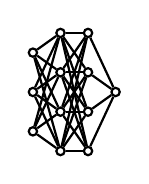
\begin{tikzpicture}[x=0.35cm,y=0.5cm]
  \readlist\Nnod{3,4,4,1} % number of nodes per layer
  % \Nnodlen = length of \Nnod (i.e., total number of layers)
  % \Nnod[1] = element (number of nodes) at index 1
  \foreachitem \N \in \Nnod{ % loop over layers
    % \N     = current element in this iteration (, , i.e.,, number of nodes for this layer)
    % \Ncnt  = index of current layer in this iteration
    \foreach \i [evaluate={\x=\Ncnt; \y=\N/2-\i+0.5; \prev=int(\Ncnt-1);}] in {1,...,\N}{ % loop over nodes
      \node[mynode] (N\Ncnt-\i) at (\x,\y) {};
      \ifnum\Ncnt>1 % connect to previous layer
        \foreach \j in {1,...,\Nnod[\prev]}{ % loop over nodes in previous layer
          \draw[thick] (N\prev-\j) -- (N\Ncnt-\i); % connect arrows directly
        }
      \fi % else: nothing to connect first layer
    }
  }
  % \draw[draw=black] (0.5,-2) -- (4.5,-2) -- (4.5,2) -- (0.5,2) -- (0.5,-2);
\end{tikzpicture}
}

% Figure environment removed 

\subsection{Optimization Problem Forms}
\label{subsec:examples}
\iffalse
\rev{Rework into a 'Problem Forms / CHallenges' section with examples illustrating LP/MIP/nonlinear and their specific challenges}

\senne{I feel like this subsection needs some reframing. I think that we should have a discussion to determine what exactly we are giving illustrations/motivations/examples of here. Is this linear programming or is it the Predict-Then-Optimize problem setting (which I think we should also explicitly name as such; see my comment in the beginning of subsection~\ref{subsec:problem_description})? I think that the latter makes the most sense and that we should reframe most of the content in this subsection.}\jay{In the last meeting, we decided to broaden the scope and include non-linear optimization problem also. This requires a bit of more works, We have to describe other optimization problems too. One limitation is we experiment only with LPs or MIPs.}
\fi
The effectiveness of solving an optimization problem depends on the specific forms of the objective and constraint functions. Considerable effort has been made to developing efficient algorithms for certain optimization forms. 
Below, the readers are provided an overview of the key and widely utilized types of optimization problem formulations.
\subsubsection{Convex optimization}
In \textit{convex} optimization problems, a convex objective function is to be optimized over a convex feasible space. This class of problems is distinguished by the guarantee that any locally optimal is also globally optimal \cite{boyd2004convex}. Since many optimization methods converge provably to local minima, convex problems are considered to be reliably and efficiently solvable relative to \emph{nonconvex} problems. Despite this, convex optimization mappings still impose significant computational overhead on Algorithm~\ref{alg:decision_focused} since they must be solved for each data sample in each epoch, and most convex optimizations are orders of magnitude more complex than conventional neural network layers \cite{amos2017optnet}. Like all parametric optimization problems, convex ones  are implicitly defined mappings from parameters to optimal solutions, lacking a closed form that can be differentiated directly. However as detailed in Section \ref{sect:kkt}, they can be canonicalized to a standard form, which facilitates automation of their solution and backpropagation by a single standardized procedure \cite{agrawal2019differentiable}.

The class of convex problems is broad enough to include some which yield mappings $\mathbf{x}^\star(\mathbf{\hat{c}})$ that are differentiable everywhere, and some which do not. The \emph{linear programs}, which are convex and form nondifferentiable mappings with respect to their objective parameters, are notable examples of the latter case and are discussed next. The portfolio optimization problem \eqref{eq:portfolio}, which contains both linear and quadratic constraints, provides an example of a parametric convex problem which admits useful gradients over some regions of its parameter space and not others. Where the (quadratic) variance constraint \eqref{eq:portfolio_ineq} is not active, it behaves as a linear program. Elsewhere, the optimal solution is a smooth function of its parameters. 

\subsubsection{Linear programming}
\label{subsubsec:linear_programming}
\emph{Linear programs} (LPs) are convex optimization problems whose objective and constraints are composed of affine functions. These programs are predominant as decision models in operations research, and have endless industrial applications since the allocation and transfer of resources is typically modeled by linear relationships between variables \cite{bazaraa2008linear}. The parametric LPs considered in this manuscript take the following form: 
\begin{subequations}
    \label{eq:param_LP}
\begin{align}
   \label{eq:param_LP_obj}
   \mathbf{x}^\star(\mathbf{c}) = \argmin_{\mathbf{x}} \mathbf{c}^\top \mathbf{x}\\
    \label{eq:param_LP_eq}
    \text{s.t.} \;\;A\mathbf{x} = \mathbf{b} \\
    \label{eq:param_LP_ineq}
    \mathbf{x} \geq \mathbf{0}
\end{align}
\end{subequations}
\noindent
Compared to other classes of convex problems, LPs admit efficient solution methods, even for large-scale problems \cite{bazaraa2008linear,ignizio1994linear}. From a DFL standpoint, however, LPs pose a challenge, because the mapping $\mathbf{c} \rightarrow \mathbf{x}^\star(\mathbf{c} )$ is nondifferentiable. Although the  derivatives of mapping     \eqref{eq:param_LP} are defined almost everywhere, they provide no useful information for gradient descent training. To see this, first note the well-known fact that a linear program always takes its optimal value at a vertex of its feasible set \cite{bazaraa2008linear}. Since the number of vertices in any such set is finite,      \eqref{eq:param_LP} maps a continuous parameter space to a discrete set of solutions. As such, it is a piecewise constant mapping. Therefore its derivatives are zero almost everywhere, and undefined elsewhere. Prevalent strategies for incorporating linear programs in decision-focused learning thus typically rely on differentiating smooth approximations to the LP, as detailed in Section~\ref{sec:analytical_smoothing}.

Many operations research problems, such as the allocation and planning of resources, can be modeled as LPs. Also many prototypical problems in algorithm design (e.g., sorting and top-\textit{k} selection) can be formulated as LPs with continuous variables, despite admitting only discrete integer solutions, by relying on the total unimodularity of the constraint matrices \cite{bazaraa2008linear}.
In what follows, some examples of machine learning models of LPs and how they might occur in a Predict-Then-Optimize context are given.
\begin{description}
    \item[Shortest paths.] Given a directed graph with a given start and end node, the goal in the shortest path problem is to find a sequence of arcs of minimal total length that connects the start end the end node. The decision variables are binary indicators of each edge's inclusion in the path. The linear constraints ensure $[0,1]$ bounds on each indicator, as well as flow balance through each node. These flow balance constraints capture that, except for the start and end node, each node has as many incoming selected arcs as outgoing selected arcs. For the start node, there is one additional outgoing selected arc, and for the end node, there is one more incoming selected arc. The parameters in the linear objective represent the arc lengths. In many realistic settings---as well as in several common DFL benchmarks \cite{elmachtoub2022smart,PogancicPMMR20}---these are unknown, requiring them to be predicted from features before a shortest path can be computed. This motivating example captures the realistic setting in which the shortest route between two locations has to be computed, but in which the road traversal times are uncertain (due to unknown traffic conditions, for example), and have to be predicted from known features (such as day of the week, time of day and weather conditions).
    
  \item[Bipartite matching.] 
    Given is a graph consisting of two sets of nodes, and arcs connecting each node of the first set to each node of the second. The arcs are weighted but the weights are unknown and must be predicted. The optimization task is to choose a subset of arcs such that each node from each set is involved in a selected arc at most once, and the total weight of the selected arcs is maximized. The variables lie in $[0,1]$ and indicate the inclusion of each edge. The constraints ensure that each node is involved at most once in a selected arc. The objective parameters represent arc weights. With a complete bipartite graph, matchings can be construed as permutations, and are presented a permutation matrices, which can be employed in tasks such as learning to rank \cite{kotary2022end}.
  
  \item[Sorting and Ranking.] The sorting of any list of predicted values can be posed as a linear program over a feasible region whose vertices correspond to all of the possible permutations of the list. The related ranking, or argsort problem assigns to any length-$n$ list a permutation of sequential integers $[n]$ which sorts the list. By smoothing the linear program, these basic operations can be differentiated and backpropagated \cite{blondel2020fast}.


  \item[Top-$k$ selection.] 
    Given a set of items and item values that must be predicted, the task is to choose the subset of size $k$ with the largest total value in selected items. In addition to $[0,1]$ bounds on the indicator variables, a single linear constraint ensures that the selected item indicators sum to $k$. A prevalent example can be found in multilabel classification \cite{amos2019limited,martins2016softmax}.
 
  
  \item[Computing the maximum.] 
   This is a special case of top-$k$ selection where $k=1$. When the LP's objective is regularized with the entropy term $H(\mathbf{x} ) = \mathbf{x} \cdot \log \mathbf{x}$, the mapping from predicted values to optimal solutions is equivalent to a softmax function \cite{agrawal2019differentiable}. 
  
  \item[Max-flow/ min-cut.] Given a network with predefined source and sink nodes, and predicted flow capacities on each arc, the task is to find the maximum flow rate that can be channeled from source to sink. Here the predicted flow capacities occupy the right-hand side of the linear constraints, which is not in line with the DFL problem description given in subsection~\ref{subsec:problem_description}. However, in the related min-cut problem---which is equivalent to the dual linear program of the max-flow problem---the flow capacities are the parameters in the objective function. The max-flow problem can thus be cast as an equivalent min-cut problem and DFL can be used to learn to predict the flow capacities. 
\end{description}
\subsubsection{Integer linear programming}
Integer Linear Programs (ILPs) are another mainstay in operations research and computer science. ILPs differ from LPs in that the decision variables $\mathbf{x}$ are restricted to integer values, i.e., $\mathbf{x} \in \mathbb{Z}^k$ where $\mathbb{Z}^k$ is the set of integral vectors of appropriate dimensions. Like LPs, ILPs are challenging to use in DFL because they yield discontinuous, nondifferentiable mappings. Computationally however, they are more challenging due to their NP-hard complexity, which may preclude the exact computation of the mapping $\mathbf{\hat{c}} \rightarrow \mathbf{x}^\star(\mathbf{\hat{c}})$ at each step of Algorithm \ref{alg:decision_focused}. Their differentiation is also significantly more challenging, since the discontinuity of their feasible regions prevents many smoothing techniques that can be applied in DFL with LPs.

In the following, examples of how ILPs may occur in a Predict-Then-Optimize setting are provided.
\begin{description}
  \item[Knapsack.] The knapsack problem has been used as a benchmark in several papers about DFL \cite{mandi2020smart,mandi2020interior,demirovic2019investigation}. Given are weights of a set of items, as well as a capacity. The items also have associated values, which have to be predicted from features. The optimization task involves selecting a subset of the items that maximizes the sum of the weights associated with the selected items, whilst ensuring that the sum of the associated weights does not exceed the capacity.
  \item[Travelling salesperson problem]
  In the travelling salesperson problem, the list of cities, and the distances between each pair of cities, is given. The goal is to find a path of minimal length that visits each city exactly once. In the Predict-Then-Optimize setting, the distances between the cities first have to be predicted \cite{PogancicPMMR20} from observable empirical data.
  \item[Combinatorial portfolio optimization.]
  Portfolio optimization involves making optimal investment decisions across a range of financial assets. In the combinatorial Predict-Then-Optimize variant, the decisions are discrete, and must be made on the basis of the predicted next period's increase in the value of several assets \cite{aaaiFerberWDT20}.
  \item[Diverse bipartite matching.]
  Diverse bipartite matching problems are similar to the bipartite matching problems described in \ref{subsubsec:linear_programming}, but are subject to additional diversity constraints \cite{aaaiFerberWDT20,mulamba2020discrete,mandi22-pmlr} In this variant, edges have additional properties. The diversity constraints enforce lower and upper bounds on the proportion of edges selected with a certain property. This precludes the LP formulation, and makes the use of ILP more interesting.
  \item[Energy-cost aware scheduling.]
  Energy-cost aware scheduling involves scheduling a set of tasks across a set of machines in a way that minimizes the overall energy cost involved. As future energy costs are unknown, they first have to be predicted \cite{mulamba2020discrete,mandi2020smart,mandi22-pmlr,mandi2020interior}.
\end{description}


\subsubsection{Integer nonlinear programming}
In integer nonlinear programming, the objective function and/or the constraints are nonlinear. Performing DFL on integer nonlinear programs faces the same challenges as performing DFL on ILPs: integer nonlinear programs are computationally expensive to solve, are implicit mappings with zero-valued gradients almost everywhere, and have discontinuous feasible regions, hindering the use of the smoothing techniques that can be applied in DFL with LPs. Additionally, because of their nonlinear nature, many of the techniques developed for DFL with ILPs, which assume linearity, do not work on integer nonlinear programs \cite{elmachtoub2022smart,PogancicPMMR20}. To the best of our knowledge, no DFL method has specifically been developed for or tested on integer nonlinear programs. The most closely related work is \cite{ferber2022surco}, which learns an approximate ILP surrogates for integer nonlinear programs, which could then in turn be used in a DFL loop.


\iffalse
We remark that to apply decision-focused learning, we have to know the structure of the optimization program. 

We train the model to generate predictions which would result in good solution of the given optimization program. The goal of decision-focused learning is \emph{not} to deliver high-quality decisions for any optimization problem. If we train the model with respect to one optimization program, it is not expected to work well for other optimization programs. \rev{I think this paragraph goes without saying, maybe leave it out?}
\fi

\iffalse
If the coefficients $\mathbf{c}$ are known exactly, existing approaches developed in the optimization community can be used to efficiently solve the problem. In such scenarios, we will call $\mathbf{x}^\star (\mathbf{c})$ the \emph{full-information optimal decision} \cite{bertsimas2020predictive}. 
In this survey, we instead consider problems where the coefficients $\mathbf{c}$ are unknown; but estimates $\mathbf{ \hat{c} }$ can be inferred from the set of observable feature variables $z$, which are correlated with $\mathbf{c}$. Then, we can make a decision $\mathbf{x}^\star ( \mathbf{ \hat{c}} )$ using the predictions.
We will call this \emph{prescriptive decision}.
The aim is to generate predictions $\mathbf{x}^\star ( \mathbf{ \hat{c}} )$ whose objective value in practice , i.e., $c^\top \mathbf{x}^\star ( \mathbf{ \hat{c}} ) $ comes close to the full-information optimal value $c^\top \mathbf{x}^\star (\mathbf{c})$.
The difference between these two is the error after the optimization step. We will call this error the \emph{task loss} \cite{emircpaior19,DontiKA17} \senne{I don't fully understand the choice of reference here. This reference in turn references 'Task-based End-to-end Model Learning in Stochastic Optimization' for the name 'task loss'. Shouldn't we refer to this one as well?} \jay{I am citing both of them for now}, to differentiate it from the \emph{prediction loss}, which captures the prediction error between $\mathbf{c}$ and $\mathbf{ \hat{c} }$.
One intuitive choice of task loss is the \emph{regret} after the downstream optimization task. \senne{I feel that by defining the task loss as the difference between $f(c,\mathbf{x}^\star ( \mathbf{ \hat{c}} ))$ and $f(c,\mathbf{x}^\star ( \mathbf{c}))$ (as done above), we define it to be equal to the regret, whereas in the previous sentence we frame the task loss as a more general concept for which the regret can be one choice. I prefer the second option: the task loss is a general concept for which the regret is one option. We should clarify this above, though.} Regret is the difference between the full-information optimal value and the objective value realized by using the predicted coefficients.
We can formally define regret in the following form
\begin{equation}
\textit{Regret}(\mathbf{x}^\star(\mathbf{\hat{c}}) )= c^\top \Big( \mathbf{x}^\star(\mathbf{\hat{c}}) - \mathbf{x}^\star (\mathbf{c}) \Big)
\label{eq:regret}
\end{equation}

The problem description, mentioned above, falls under the category of supervised machine learning problems, where past observations $\{ (\mathbf{z_i},  \mathbf{c_i})  \}_{i=1}^N$ are available to learn ML models $m_{\bm{\omega}}$ (with parameters $\bm{\omega}$). \senne{What do we mean with 'sounds similar' here? It \textit{is} a supervised learning problem.} \jay{Absolutely right, changed} During inference time, given a feature vector $z$, the outputs of the ML model $m_{\bm{\omega}}(z)$ $(=\hat{c})$ serve as estimates of the coefficients $\mathbf{c}$.

\senne{What follows does not belong in the "The Problem Description" section anymore, in my opinion. It is not a description of the problem anymore, but an introduction to typical approaches to solving the problem.}The straight-forward approach to this supervised ML problem is to train the model to generate accurate predictions $\mathbf{ \hat{c} }$. We call this approach \emph{prediction-focused} (also called the two-stage \cite{aaai/WilderDT19}) learning because here the model is trained with a focus on the predictions. As shown in Algorithm~\ref{alg:prediction_focused}, In this setup, the ML model is trained to minimize the \emph{prediction loss} between $\mathbf{c}$ and $\mathbf{ \hat{c} }$. 
Clearly, in this case, the model training is agnostic of the downstream optimization problem. For instance, if we train with respect to mean square error (MSE), we would minimize the following loss
\begin{equation}
    \min \frac{1}{N} \sum_{i=1}^N \bigg( c_i - \hat{c}_i \bigg)^2
    \label{eq:prediction_focused}
\end{equation}

Modern deep learning architectures train the ML models by stochastic gradient-descent (SGD), where $\bm{\omega}$ is iteratively updated in the opposite direction of the gradient of the of the loss function with respect to $\bm{\omega}$.

During inference, after making the predictions $\hat{c} $, they are passed to optimization solvers, which solves \eqref{eq:LP} to return $\mathbf{x}^\star ( \mathbf{ \hat{c}} )$.
\paragraph{Decision-Focused Learning} 
\senne{I like the use of the paragraph environment here, but think that we should do the same for 'prediction-focused learning'.} As we mentioned before, in prediction-focused learning, we train the model without taking the optimization task into consideration.
It assumes that generating accurate predictions will result in good prescriptive decisions. Of course this is true when the predictions are fully correct, but this is impossible in practice. 
When the ML model makes prediction errors, the prediction-focused learning does not take the impact of the error in the prescriptive decision into account. \senne{This is repetition}
The impact of prediction error is not uniform throughout the solution space. For instance, let us consider the weighted knapsack problem, where we have to predict the values of each item. If the weights of an item is greater than the capacity of the knapsack, that item would not feature in the solution, regardless of the values predicted. Therefore prediction error of that item does not impact the solution, whereas errors of other items would have impacts. \senne{This is true but feels like a trivial case; I don't think that this would really convince the reader that the mapping between prediction and decision errors can be really complex.} \jay{Should I provide  a small example in tabular form, to be discussed.}

The decision-focused learning paradigm aims to overcome this weakness by considering the optimization problem while training the predictive model.
The goal of decision-focused learning is to train the ML models with respect to the quality of the decisions made on the basis of the predicted coefficients.
Decision-focused learning achieves this by integrating the optimization program into the training loop of the ML model. 
To do so, the ML model is trained to directly minimize the \emph{task loss}, rather than the \emph{prediction loss}, as commonly done in an ML setup. 
Conceptually, in this paradigm, generating the predicted  coefficient $\mathbf{ \hat{c} }$ is the intermediary step and accuracy of this step is not the primary focus. The focus, rather, is on the error after the optimization. As mentioned before, one possible way to quantify the task loss is by using \emph{regret}.
We conceptually explain the decision-focused paradigm to minimize regret in Algorithm~\ref{alg:decision_focused}. Here after predicting the coefficient $\mathbf{ \hat{c} }$, we have to compute its solution $\mathbf{x}^\star ( \mathbf{ \hat{c}} )$, followed by evaluating the regret (line 6 in Algorithm~\ref{alg:decision_focused}) and then to update the model parameter $\bm{\omega}$ to minimize regret.
The training objective of minimizing the regret in decision-focused learning paradigm, may also be expressed in the following bilevel optimization form
\begin{align}
    \min_{\bm{\omega}} \frac{1}{N} \sum_{i=1}^N \Big( c_i^\top \big(\mathbf{x}^\star( \hat{c}_i ) - \mathbf{x}^\star(c_i) \big) \Big) \label{eq:bilevel_outer}\\
    \text{such that } \hat{c}_i = m_\bm{\omega} (z_i)  ;\ \mathbf{x}^\star( \hat{c}_i ) = \argmin_{x \geq 0; Ax=b} \hat{c}_i^\top x 
    \label{eq:bilevel_inner}
\end{align}
The outer level problem \eqref{eq:bilevel_outer} minimizes the regret on the training set and the inner level problem \eqref{eq:bilevel_inner} finds the optimal solution of each predicted coefficients. 
However, solving \eqref{eq:bilevel_outer} is more arduous than solving \eqref{eq:prediction_focused} in the prediction-focused paradigm. 

We remark that to apply decision-focused learning, we have to know the structure of the optimization program. 
We train the model to generate predictions which would result in good solution of the given optimization program. The goal of decision-focused learning is \emph{not} to deliver high-quality decisions for any optimization problem. If we train the model with respect to one optimization program, it is not expected to work well for other optimization programs.
\fi





% \section{Illustrations/ Motivations/ Examples }
% \senne{My preference: place this section elsewhere in the paper. General order: Predict-Then-Optimize problem setting, then motivating examples (this section), then prediction- vs decision-focused learning, then challenges of DFL.}
% Linear programming is a mainstay of operations research modeling, due to the linearity of many relationships that model allocation and planning of resources, and the prevalence of efficient solution methods even for large scale problems. More broadly, many prototypical problems in algorithm design can also be formulated as linear programs. 

% \begin{description}
%     \item[Shortest paths.] For a graph $G= (V,E)$, the problem of finding the fastest path from vertex $s$ to vertex $t$ can be written as \eqref{eq:LP}, where travel times between the vertices form the cost coefficient vector. The task is to first predict the travel time vector, and then recommend the fastest  path using these travel times. 
%   \item[Bipartite matching problems.] Bipartite matching can be used to match two sets of vertices, such as matching recruiters with job-seekers. In such cases, the coefficient vector includes the reward of matching any two vertices. The task is to first predict those rewards for all pairs of vertices, and to then determine which vertices to be matched so as to maximize the total reward.
%   \item[Computing the maximum.] One common task in ML classification is to return class with the largest probability from a set of $k$ classes. This can be
%   formulated as decision-focused learning task, where the prediction task is to generate the probabilistic predictions and the optimization task is to return the class with highest probability.
%   \item[Top-$k$ selection.] Here the task is to choose a subset of items from a given set. This can be formed as a linear optimization problem, where the input is the vector of probabilistic predictions of membership of each item and the is a set of binary vectors indicating membership.\senne{This needs some work. What is meant with the "probabilistic predictions of membership"? Also, what is the objective in the item selection?}
  
%   \item[Sorting and Ranking.]
  
%   \item[Minimum spanning tree.] For an undirected graph $G= (V,E)$, the minimum spanning tree is an acyclic subset of edges that connects all the vertices together, such that the sum of the selected edges' weights is minimal. We can formulate the problem of computing this tree as an ILP, which takes the predicted edge weight as inputs and returns the binary indicator vectors of the edges selected in the spanning tree.

% %   \item[Hyperparameter Optimization.]
% \end{description}
% \section{Challenges of Decision-focused Learning}
% \rev{JK: I would vote for bringing this whole section under section 4, and using this little subsection as an introduction/preamble.}

% \label{sec:challenges}
% In the previous section, we argue why DFL is desirable to tackle problems with prediction and optimization. Now, we turn towards the challenge of implementing DFL. 
% % Figure environment removed

% \subsection{The Challenge of Backpropagating through Optimization Mapping}\label{sect:differentiability}
% SGD is the backbone of training ML, especially neural network models. In order to train an ML model, the model parameters are updated in the backward pass.\senne{We should either not give this context, or expand it (in a separate section). Somehow who is not familiar won't know what 'the backward pass' means, and for someone who is famliliar this information is redundant. Perhaps a preliminary section with a basic introduction to gradient-based training of predictive models would be a nice addition to the survey.} In the backward pass of SGD, first the derivatives of the loss function with respect to the model parameters are computed and then the parameters are updated in the direction of the derivative (line 6 in Algorithm~\ref{alg:prediction_focused}). \senne{This should be in the direction \textit{opposite} to the derivative.} This can be easily performed in any modern deep learning architecture such as PyTorch and TensorFlow. 
% However, computing this derivative is not straight forward in the decision-focused learning paradigm.
% In this setup, 

% \paragraph{Differentiating through an LP}
% \senne{After discussion in meeting: this discussion of the KKT conditions will go to section 5}
% In an LP, the mapping from $\mathbf{c}$ to $\mathbf{x}^\star (\mathbf{c})$ is piecewise constant, because a small change in $\mathbf{c}$ typically does not change $\mathbf{x}^\star (\mathbf{c})$, and when it does, it does the solution suddenly jumps from one vertex to another. So, the derivative $\frac{ d \mathbf{x}^\star ( \mathbf{ \hat{c}} )}{ d \mathbf{ \hat{c} }}$ is zero almost everywhere, and undefined where it is not.
% For a continuous problem, the optimal solution satisfies the KKT conditions, so it seems plausible to apply the implicit function theorem to differentiate the KKT linear equations. However, for an LP \eqref{eq:LP}, this is not possible. We show this in what follows.

% To write down the KKT conditions, first we write the Lagrangian relaxation function of the problem.
% The Lagrangian relaxation function of an optimization problem with objective $f(c,x)$ and linear constraint $Ax=b$ takes the following form

% \rev{JK note to self: regret or 'task loss' based learning only makes sense when only the objective is parameterized. Make sure this is made clear somewhere}

% \begin{equation}
% \mathbb{L}(x,y;c) = f(c,x) + y^\top (b -Ax)
% \label{eq:Lagrangian}
% \end{equation}
% where $y$ is a Lagrange multiplier.
% Notice \eqref{eq:LP} is a special case, where $f(c,x) = c^\top x$.

% The KKT conditions, which are necessary for optimality, can be obtained by differentiating \eqref{eq:Lagrangian}
% \begin{align}
% \begin{split}
% f_{x} (c,x) - A^\top y & = 0 \\
% A x -b & =0
% \end{split}
% \label{eq:KKT}
% \end{align}

% The implicit differentiation of the KKT linear equations with respect to $\mathbf{c}$ produces following system of equalities:
% \begin{align}
% \begin{bmatrix}
% f_{cx} (c,x)\\
% 0\\
% \end{bmatrix}
% +
% \begin{bmatrix}
% f_{xx} (c,x) & -A^\top \\
% A & 0\\
% \end{bmatrix}
% \begin{bmatrix}
% \frac{d }{d  c}   x\\
% \frac{d }{d  c}   y\\
% \end{bmatrix}
% = 0
% \label{eq:implicit_differentiation}
% \end{align}
% System \eqref{eq:implicit_differentiation} can be solved if 
% $f_{xx} (c,x)$ is non-zero, i.e., $f(c,x)$ \rev{is twice-differentiable}. But the LP optimization \rev{problem} in \eqref{eq:LP} is not twice-differentiable. 
% Conceptually, the derivative of $\mathbf{x}^\star ( \mathbf{c})$ with respect to $\mathbf{c}$ does not exist for an LP optimization problem, because the solution always lies on a vertex or it is a face.\senne{Again, should we state this? I think that it does exist most of the time, but is just zero.}

% As $\frac{ d \mathbf{x}^\star ( \mathbf{ \hat{c}} )}{ d \mathbf{ \hat{c} }}$ \rev{does not exist} for an LP optimization problem, different approaches have been proposed in the literature to obtain an useful gradient. We will cover them in detail in section \ref{sect:review}.
% \jk{JK TODO: let's show why the differential KKT conditions for LP are singular, discuss why the QP and cone differential KKT's are 'solvable', and a brief mention of the cone transformations approach for general convex. In this paper, general convex diff is used for entropy-regularized LP}

% \citeA{mulamba2020discrete} and \citeA{mandi22-pmlr} aim to address this in their works, which we will describe in detail in section \ref{sect:review}.
% % Figure environment removed


\section{Review of Decision-focused Learning Methodologies}\label{sect:review}
To the best of our knowledge, this manuscript is the first to provide a comprehensive review of methods developed for and suitable for DFL in gradient-based training.
Concurrently with this paper, \citeA{sadana2023survey} survey recently proposed approaches to address Predict-Then-Optimize problems (referred to as contextual optimization within it). While \citeA{sadana2023survey} also cover some of the works to be surveyed later, this manuscript goes beyond by presenting an extensive review solely focused on DFL methods and proposing the first categorization of existing DFL methods.


This section will describe several methodologies which address the challenge of differentiating an optimization mapping for DFL in gradient-based training.
% In the previous section, we explained why it is not possible to directly minimize regret for training. 
% To overcome this, various decision-focused learning approaches propose different surrogate loss functions, resulting in differentiable gradients or sub-gradients. 
In essence, different approaches propose different smoothed surrogate approximations of $\frac{ d  \mathbf{x}^\star (\mathbf{\hat{c}})}{ d  \mathbf{\hat{c}}}$ or $\frac{ d  \mathcal{L}(\mathbf{x}^\star (\mathbf{\hat{c}}))}{ d \mathbf{ \hat{c}}}$, which is used for backpropagation. 
% At this point, it is worth noting that some of the approaches consider the true coefficients $\mathbf{c}$ as latent variables and do not necessarily use the true coefficient for training the ML model.
% \tias{Intro and conclusion talk about '5 categories', but they do not "jump out" of the paper. It are the subsections here, right? They should be summarized here in the intro of the section, e.g. with an enumerated list or in a table or so, visually standing out.}
\raggedbottom
This paper proposes the first categorization of existing DFL approaches into the following four distinct classes:
\begin{description}
    \item [Analytical Differentiation of Optimization Mappings:] Methodologies under this category aim to compute exact derivative for backpropagation by differentiating the optimality conditions for certain optimization problem forms, for which the derivative exists and non-zero.
    \item [Analytical Smoothing of Optimization Mappings:] These approaches deal with combinatorial optimization problems (for which the analytical derivatives are zero almost everywhere) by performing smoothing of combinatorial optimization problems, which results in approximate problems that can be differentiated analytically.
    \item [Smoothing by Random Perturbations:] Methodologies under this category utilize implicit regularization through perturbations, constructing smooth approximations of optimization mappings.
    \item [Differentiation of Surrogate Loss Functions:] Methodologies under this category propose convex surrogate loss functions of specific task loss such as regret. 
    \item [Decision-Focused Learning without Optimization in the Loop:] 
    These methodologies bypass the need for computing $\frac{ d  \mathcal{L}(\mathbf{x}^\star (\mathbf{\hat{c}}))}{ d \mathbf{ \hat{c}}}$ by utilizing surrogate losses, which reflect the quality of the decisions, but do not require computing the solution of the optimization problem for differentiation.
\end{description}
\raggedbottom
Figure~\ref{Fig:DFLMethodologyTable} presents key characteristics of these four methodology classes, 
highlighting the types of problems that can be addressed within each class. 
Next, each category is thoroughly described.

\tikzset{
  table/.style={
    matrix of nodes,
    row sep=0.1\pgflinewidth,
    column sep=-\pgflinewidth,
    nodes={
      rectangle,
      draw=black,
      align=center,
      minimum height=\baselineskip, % Adjust the height as needed
       text width = 0.12\textwidth, text depth = 16mm, text
    height = 3mm, draw, text centered, anchor=south, font=\small 
    },
    nodes in empty cells,
  %    column 1/.style={
  %           nodes={
  %     draw=black
  %   }
  % },
   column 1/.style={
            nodes={draw=black, text width = 0.2\textwidth, font=\bfseries}
        },
   column 2/.style={
   	nodes={draw=black, text width = 0.15\textwidth}
   },
      column 3/.style={
   	nodes={draw=black, text width = 0.16\textwidth}
   },
  row 1/.style={
           nodes={
                fill=black,
                text=white,
                text depth = 5mm,
                text height = 2mm,
                font=\bfseries
            },
            }
},
arrow/.style={thick,->,>=stealth}
}
\begin{center}
% Figure environment removed 
\end{center}
% \iffalse
% The KKT conditions 

% - The methods of the section apply when differentiating the solution to an optimization problem with respect to any of its defining parameters

% - KKT conditions characterize local optimality of nonlinear programs 

% - For convex problems, the KKT conditions characterize global optimality - 'sufficient' conditions

% - Emphasize that in this section we are computing exact gradients, not approximations

% - For linear programming, the approximation enters when smooth surrogate terms are introduced to the optimization model

% - Not all differentiated KKT conditions are easy to solve (for the same reasons that not all KKT conditions themselves are easy to solve)

% - Differentiated KKT conditions are linear when the underlying program is quadratic in objective and constraints

% - LP is a special case of QP - the diff KKT matrix has a block zero diagonal
% \\
% \\
% \fi
% \iffalse
% Differentiation of optimization problems for sensitivity analysis dates back several decades and is treated thoroughly in \cite{bonnans2013perturbation}. \senne{I don't see how the first sentence ties to the second. Won't it benefit this section to drop the first sentence?}
% \fi
\raggedbottom
\subsection{Analytical Differentiation of Optimization Mappings}
\label{sect:kkt}
As discussed before, differentiating through parametric CO problems comes with two main challenges. First, since CO problems are complex, implicitly defined mappings from  parameters to solutions, computing the derivatives is not straightforward. Second, since some CO problems result in piecewise-constant mappings, their derivatives are zero almost everywhere, and do not exist elsewhere.
\raggedbottom

This subsection pertains to CO problems for which the second challenge does not apply, i.e., problems that are smooth mappings. For these problems, all that is required to implement DFL is direct differentiation of the mapping in Eq.~\eqref{eq:opt_generic}.
\paragraph{Differentiating unconstrained relaxations.}
An early work discussing differentiation through constrained argmin problems in the context of machine learning is \cite{gould2016differentiating}. It first proposes a technique to differentiate the argmin of a smooth, \textit{unconstrained} convex function. When $V(\mathbf{c}) = \argmin_{\mathbf{x}} f(\mathbf{c}, \mathbf{x})$, it can be shown that when all second derivatives of $f$ exist, 
\begin{equation}
 \frac{dV(\mathbf{c})}{d \mathbf{c}} = - \frac{f_{\mathbf{cx}}( \mathbf{c},V(\mathbf{c}))}{f_{\mathbf{xx}}( \mathbf{c},V(\mathbf{c}))}
\end{equation}
where $f_{ \mathbf{cx}}$ is the second partial derivative of $f$ with respect to $\mathbf{c}$ followed by $\mathbf{x}$. This follows from implicit differentiation of the first-order optimality conditions
\begin{equation}
 \frac{df}{d \mathbf{x}}(\mathbf{c},V(\mathbf{c})) = 0
\end{equation}
with respect to $\mathbf{c}$, and rearranging terms. Here the variables $\mathbf{c}$ are the optimization problem's defining parameters, and the variables $\mathbf{x}$ are the decision variables.

This technique is then extended to find approximate derivatives to \textit{constrained} problems with inequality constraints $g_i(\mathbf{c}, \mathbf{x}) \leq 0$, $1 \leq i \leq m$, by first relaxing the problem to an unconstrained problem, by means of the log-barrier function
\begin{equation}
 F(\mathbf{c},\mathbf{x}) =  f(\mathbf{c},\mathbf{x}) - \mu \sum_i \log(-g_i(\mathbf{c},\mathbf{x}))
\end{equation}
and then differentiating $\argmin_{ \mathbf{x} } F(\mathbf{c},\mathbf{x})$ with respect to $\mathbf{c}$ for some choice of the scaling factor $\mu$. Since this approach relies on approximations and requires hyperparameter tuning for the factor $\mu$, subsequent works focus on differentiating constrained optimization problems directly via their own global conditions for optimality, as discussed next. 

\paragraph{Differentiating KKT conditions of quadratic programs.}
More recent approaches are based on differentiating the optimality conditions of a CO problem directly, i.e., without first converting it to an unconstrained problem. Consider an optimization problem and its optimal solution:
\begin{subequations}
    \label{eq:general_convex}
\begin{align}
  \label{eq:general_convex_objective}
    \mathbf{x}^\star   = \argmax_{\mathbf{x}} &\;\;
    f(\mathbf{x})\\
    \label{eq:general_convex_inequality}
    \texttt{s.t.} &\;\;
    \bm{g}(\mathbf{x}) \leq 0 \\
    \label{eq:general_convex_equality}
     & \;\; \bm{h}(\mathbf{x}) = 0
\end{align}
\end{subequations}
\iffalse
Consider an optimization problem viewed as a mapping from parameters $\mathbf{c}$ which define its objective and constraint functions, to a resulting optimal solution:
\begin{subequations}
    \label{eq:general_convex_param}
\begin{align}
  \label{eq:general_convex_objective_param}
    \mathbf{x}^\star (\mathbf{c})   = \argmax_{ \mathbf{x} } &\;\;
    f(x)\\
    \label{eq:general_convex_inequality_param}
    \texttt{s.t.} &\;\;
    g(x,c) \leq 0 \\
    \label{eq:general_convex_equality_param}
     & \;\; h(x,c) = 0
\end{align}
\end{subequations}
\fi
and assume that $f$, $g$ and $h$ are differentiable functions of $\mathbf{x}$. The Karush–Kuhn–Tucker (KKT) conditions are a set of equations expressing optimality conditions for a solution $\mathbf{x}^\star$ of problem (\ref{eq:general_convex}) \cite{boyd2004convex}:
\begin{subequations}
    \label{eq:KKT}
\begin{align}
  \label{eq:KKT_stationarity}
    \nabla f(\mathbf{x}^\star) + \sum_i w_i \nabla h_i(\mathbf{x}^\star) + \sum_j  u_j \nabla g_j(\mathbf{x}^\star) = 0\\
    \label{eq:KKT_primal_feasibility_ineq}
    g_j(\mathbf{x}^\star) \leq 0 \;\; \forall j \\
    \label{eq:KKT_primal_feasibility_eq}
    h_i(\mathbf{x}^\star) = 0 \;\; \forall i \\
    \label{eq:KKT_dual_feasibility}
    u_j \geq 0 \;\; \forall j \\
    \label{eq:KKT_complementary_slackness}
     u_j g_j(\mathbf{x}^\star) = 0  \;\; \forall j
\end{align}
\end{subequations}
\textsl{OptNet} is a framework developed by \citeA{amos2017optnet} to differentiate through optimization mappings that are convex quadratic programs (QPs) by differentiating through these KKT conditions. In convex quadratic programs, the objective $f$ is a convex quadratic function and the constraint functions $g, h$ are linear over a continuous domain. In the most general case, each of $f$, $g$ and $h$ are dependent on a distinct set of parameters, in addition to the optimization variable $\mathbf{x}$:
\begin{subequations}
    \label{eq:QP_param}
\begin{align}
  \label{eq:QP_param_f}
    f(\mathbf{c},Q, \mathbf{x}) = \frac{1}{2} \mathbf{x}^\top Q \mathbf{x} + \mathbf{c}^\top \mathbf{x}\\
    \label{eq:QP_param_g}
      g(A, \mathbf{b}, \mathbf{x}) = R \mathbf{x} - \mathbf{s }\\
    \label{eq:QP_param_h}
     h(R,\mathbf{s},\mathbf{x}) = A \mathbf{x} - \mathbf{b}
\end{align}
\end{subequations}
When $\mathbf{x} \in \mathbb{R}^k$ and the number of equality constraints is $M_{in}$ and $M_{eq}$, respectively, a QP problem is specified by parameters $Q \in \mathbb{R}^{k \times k}$,  $\mathbf{c} \in \mathbb{R}^{k}$,   $R \in \mathbb{R}^{k \times M_{in}}$, $\mathbf{s} \in \mathbb{R}^{M_{in}}$, $A \in \mathbb{R}^{k \times M_{eq}}$, and $\mathbf{b} \in \mathbb{R}^{M_{eq}}$. Note that for this problem to be convex, $Q$ must be positive-semidefinite always, which can be ensured by learning instead parameters $\mathbf{q } \in \mathbb{R}^{k}$ and taking $Q = \mathbf{q}^\top \mathbf{q}$.

A defining characteristic of quadratic programs such as \eqref{eq:QP_param} is their straightforward parameterization. This is due to the fact that any linear or quadratic function can be fully specified by a square matrix or a vector of parameters, respectively. Here, problem (\ref{eq:general_convex}) is viewed as a mapping  $(Q, \mathbf{c},R,\mathbf{s},A, \mathbf{b}) \rightarrow \mathbf{x}^\star (Q, \mathbf{c},R,\mathbf{s},A, \mathbf{b}) $, which parameterizes the space of all possible quadratic programs and their solutions. The presence of such a canonical form allows for separation of a problem's inherent structure from its parameters \cite{grant2008graph}, and is key to creating a differentiable mapping from parameters to optimal solutions in an automated way, without necessitating additional analytical transformations. 

The gradients are sought with respect to each of the parameters in $(Q, \mathbf{c},R,\mathbf{s},A, \mathbf{b}) $. For this purpose, \citeA{amos2017optnet} argue that the inequalities (\ref{eq:KKT_primal_feasibility_ineq}) and  (\ref{eq:KKT_dual_feasibility}) can be dropped, resulting in a system of equalities representing optimality conditions for $\mathbf{x}^\star$. 

Exact gradients $\frac{d \mathbf{x}^\star}{d P}$ for any $P\in \{ Q, \mathbf{c},R,\mathbf{s},A, \mathbf{b} \}$ can then be retrieved by solving the differential KKT conditions:
\begin{equation}
\label{eq:qp_differential_kkt}
\left[
\begin{matrix}  Q & R^\top & A^\top \\
                D(\bm{w}^*)R & D(R\mathbf{x}^* - \mathbf{s}) & 0 \\
                A & 0 & 0 \end{matrix}
\right]
\left[  \begin{matrix} d \mathbf{x} \\ d\bm{w}\\ d\bm{u}  \end{matrix} \right]
=
-\left[
\begin{matrix}  dQ\mathbf{x}^*  + d \mathbf{c} + dR^\top \bm{w}^* + dA^\top \bm{u}^* \\
                D(\bm{w}^*)dR \mathbf{x}^* - D(\bm{w}^*)d \mathbf{s} \\
                dA\mathbf{x}^* - d\mathbf{b} \end{matrix}
\right]
\end{equation}
where the shorthand $d$ stands for the derivative $\frac{d }{d P}$. This is another example of implicit differentiation, and requires solving a linear system of equations.
Later, \citeA{TakuyaGradientBoosting} extended the method of \citeA{amos2017optnet}, where they compute the second order derivative of the solution. This allows to train gradient boosting models, which require the gradient as well as the Hessian matrix of the loss.

%Also provided in \cite{amos2017optnet} is an efficient implementation for solving \eqref{eq:qp_differential_kkt}, based on retaining a factorization of its left-hand side matrix from the interior point algorithm that solves the QP.
In summary, the techniques in this category compute the derivatives of the solution with respect to the parameters (if they exist) by leveraging implicit differentiation of the KKT conditions.


\paragraph{Differentiating optimality conditions of conic programs.}
Another class of problems with a parametric canonical form are the conic programs, which take the form: 
\begin{subequations}
    \label{eq:cone}
\begin{align}
  \label{eq:cone_objective}
    \mathbf{x}^\star(A,\mathbf{b},\mathbf{c})   = \argmax_{ \mathbf{x} } &\;\;
    \mathbf{c}^\top \mathbf{x}\\
    \label{eq:cone_inequality}
    \texttt{s.t.} &\;\;
    A\mathbf{x} - \mathbf{b} \in \mathcal{K}
\end{align}
\end{subequations}
where $\mathcal{K}$ is a nonempty, closed, convex cone. 

A framework for differentiating the mapping (\ref{eq:cone}) for any $\mathcal{K}$ is proposed in \cite{agrawal2019coneprogram}, which starts by forming the homogeneous self-dual embedding of (\ref{eq:cone}), whose parameters form askew-symmetric block matrix composed of $A$, $\mathbf{b}$, and $\mathbf{c}$. Following \cite{busseti2019solution}, the solution to this embedding is expressed as the problem of finding a zero of a mapping containing a skew-symmetric linear function and projections onto the cone $\mathcal{K}$ and its dual. The zero-value of this function is implicitly differentiated, in a similar manner to the KKT conditions of a quadratic program as in \cite{amos2017optnet}. The overall mapping  (\ref{eq:cone}) is viewed as the composition of function that maps $(A,\mathbf{b},\mathbf{c})$ onto the skew-symmetric parameter space of the self-dual embedding, the rootfinding problem that produces a solution to the embedding, and a transformation back to a solution of the primal and dual problems. The overall derivative is found by a chain rule applied over this composition. 

Subsequent work \cite{agrawal2019differentiable} leverages the above-described differentiation of cone programs to develop a more general differentiable convex optimization solver---\textsl{Cvxpylayers}. It is well known that conic programs of the form (\ref{eq:cone}) can provide canonical representations of convex programs \cite{nemirovski2007advances}. The approach described by \citeA{agrawal2019differentiable} is based on this principle; that a large class of \emph{parametric} convex optimization problems can be recast as equivalent parametric cone programs, with an appropriate choice of the cone $\mathcal{K}$. A major benefit of this representation is that it allows a convex program to be separated with respect to its defining parameters ($A,\mathbf{b},\mathbf{c}$) and its structure $\mathcal{K}$, allowing a generic procedure to be applied for solving and differentiating the transformed problem with respect to $A$, $\mathbf{b}$ and $\mathbf{c}$. 

The framework for transforming convex programs to cone programs of the form (\ref{eq:cone}) is drawn from \cite{grant2008graph}, which is based on two related concepts. First is the notion of \emph{disciplined convex programming}, which assists the automation of cone transforms by imposing a set of rules or conventions on how convex programs can be represented. Second is the notion of \emph{graph implementations}, which represent functions as optimization problems over their epigraphs, for the purpose of generically representing optimization problems and assisting conversion between equivalent forms. The associated software system called $\texttt{cvx}$ allows for disciplined convex programs to be converted to cone programs via their graph implementations. Subsequently, the transformed problem is solved using conic optimization algorithms, and its optimal solution is converted to a solution of the original disciplined convex program. Differentiation is performed through each operation and combined by the chain rule. The transformation of parameters between respective problem forms, and the solution recovery step, are differentiable by virtue of being affine mappings \cite{agrawal2019differentiable}. The intermediate conic program is differentiated via the methods of \cite{agrawal2019coneprogram}. 

\paragraph{Solver unrolling and fixed-point differentiation.}
While the methods described above for differentiation through CO problems are generic and applicable to broad classes of problems, other practical techniques have been proven effective and even advantageous in some cases. A common strategy is that of solver \emph{unrolling}, in which the solution to \eqref{eq:opt_generic} is found by executing an optimization algorithm in the computational graph of the predictive model. Then, the mapping \eqref{eq:opt_generic} is backpropagated simply by automatic differentiation or `unrolling' through each step of the algorithm, thus avoiding the need to explicitly model $\frac{d  \mathbf{x}^{\star}(\mathbf{c} )}{d  \mathbf{c}}$ \cite{domke2012generic}. While this approach leads to accurate backpropagation in many cases, it suffers disadvantages in efficiency due to the memory and computational resources required to store and apply backpropagation over the entire computational graph of an algorithm that requires many iterations \cite{amos2017optnet}. Additionally, it has been observed that unrolling over many solver iterations can leads to vanishing gradient issues reminiscent of recurrent neural networks \cite{monga2021algorithm}. On the other hand, unrolling allows for the learning of unspecified algorithm parameters, such as gradient descent step sizes or weights in an augmented lagrangian, which can be exploited to accelerate the forward-pass convergence of the optimization solver. A comprehensive survey of algorithm unrolling for image processing applications is provided in \cite{monga2021algorithm}.

Another way in which a specific solution algorithm may provide gradients though a corresponding optimization mapping, is by implicit differentiation of its fixed-point conditions. Suppose that the solver iterations 
\begin{equation}
    \label{eq:opt_iteration}
        \mathbf{x}_{k+1}(\mathbf{c}) = \mathcal{U}(\mathbf{x}_k (\mathbf{c}) ,\;  \mathbf{c} )
\end{equation}

\noindent converge as $k \rightarrow \infty$ to a solution $\mathbf{x}^{\star}(\mathbf{c})$ of the problem \eqref{eq:opt_generic}, then the fixed-point conditions 

\begin{equation}
    \label{eq:opt_fixedpt}
       \mathbf{x}^{\star}(\mathbf{c}) = \mathcal{U}(\mathbf{x}^{\star} (\mathbf{c}) ,\;  \mathbf{c} )
\end{equation}
\noindent are satisfied. Assuming the existence of all derivatives on an open set containing $\mathbf{c}$ to satisfy the implicit function theorem, it follows  by implicit differentiation with respect to $\mathbf{c}$ that
\begin{equation}
    \label{eq:Lemma_fixedpt}  
        (I - \Phi ) \frac{d \mathbf{x}^{\star}}{d \mathbf{c}} = \Psi,
\end{equation}

\noindent which is a linear system to be solved for $\frac{d \mathbf{x}^{\star}}{d \mathbf{c}}$, in terms of   $\Phi = {{\frac{d \mathcal{U} }{d \mathbf{x}^{\star}} (\mathbf{x}^{\star}(\mathbf{c}), \; c )}}$ and  $\Psi = \frac{d \mathcal{U} }{\mathbf{c}} (\mathbf{x}^{\star}(\mathbf{c}), \; \mathbf{c})$.


\noindent The relationship between unrolling and differentiation of the fixed-point conditions is studied by \citeA{kotary2023folded}, which shows that backpropagation of \eqref{eq:opt_generic} by unrolling \eqref{eq:opt_iteration} is equivalent to solving the linear system     \eqref{eq:Lemma_fixedpt}  by fixed-point iteration. As such, the convergence rate of the backward pass in unrolling is determined by the convergence rate of the equivalent linear system solve, and can be calculated in terms of the spectral radius of $\Phi$. %This also implies that unrolling of \eqref{eq:opt_iteration} is typically inefficient compared to 









%Recent works have shown that backpropagation through the steps of an optimization solver can be harnessed more efficiently using implicit differentiation. As described above, the KKT conditions represent theoretical conditions for optimality which can be implicitly differentiated to find the derivatives through an underlying optimization-based mapping. As shown in \cite{wilder2019end,blondel2022efficient} 


\paragraph{Discussion.}
In contrast to most other differentiable optimization methods surveyed in this article, the analytical approaches in this subsection allow for backpropagation of coefficients that specify the constraints as well the objective function. For example, \citeA{amos2017optnet} propose parametric quadratic programming layers whose linear objective parameters are predicted by previous layers, and whose constraints are learned through the layer's own embedded parameters. This is distinct from most cases of DFL, in which the optimization problems have fixed constraints and no trainable parameters of their own. 

Furthermore, the techniques surveyed in this subsection are aimed at computing exact gradients of parametric optimization mappings. However, many applications of DFL contain optimization mappings that are discontinuous and piecewise-constant. Such mappings, including parametric  linear programs \eqref{eq:param_LP}, have gradients that are zero almost everywhere and thus do not supply useful descent directions for SGD training. Therefore, the techniques of this subsection are often applied after regularizing the problem analytically with smooth functions, as detailed in the next subsection. 

\subsection{Analytical Smoothing of Optimization Mappings}
\label{sec:analytical_smoothing}
To differentiate through combinatorial optimization problems, the optimization mapping first has to be smoothed. While techniques such as noise-based gradient estimation (surveyed in Section~\ref{sect:perturb}) provide smoothing and differentiation simultaneously, analytical differentiation first incorporates smooth analytical terms in the optimization problem's formulation, and then analytically differentiates the resulting optimization problem using the techniques discussed in Section~\ref{sect:kkt}.

\paragraph{Analytical smoothing of linear programs.} Note that while an LP problem is convex and has continuous variables, only a finite number of its feasible solutions can potentially be optimal. These points coincide with the vertices of its feasible polytope \cite{bazaraa2008linear}. Therefore the mapping $\mathbf{x}^\star ( \mathbf{ \hat{c}} )$ in (\ref{eq:param_LP}), as a function of $\mathbf{ \hat{c} }$, is discontinuous and piecewise constant, and thus requires smoothing before it can be differentiated through. An approach to do so was presented in
\citeA{aaai/WilderDT19}, which proposes to  augment the linear LP objective function with the Euclidean norm of its decision variables, so that the new objective takes the following form
\begin{subequations}
    \label{eq:qptl}
    \begin{align}
    \mathbf{x}^{\star}(\mathbf{c}) &= \argmax_\mathbf{x}  \mathbf{c}^\top \mathbf{x} - \mu \lVert \mathbf{x} \rVert^2_2 \\
    &= \argmin_{\mathbf{x}} \lVert \mathbf{x} - \frac{ \mathbf{c} }{\mu} \rVert^2_2
    \end{align}
\end{subequations}

\noindent where the above equality follows from expanding the square and cancelling constant terms, which do not affect the $\argmax$. This provides an intuition as to the effect of such a quadratic regularization: it converts a LP problem into that of projecting the point $\frac{ \mathbf{c}}{\mu}$ onto the feasible polytope, which results in a continuous mapping $\mathbf{\hat{c}} \to \mathbf{x}^\star(\mathbf{\hat{c}})$.  \citeA{aaai/WilderDT19} then train decision-focused models by solving and backpropagating the respective quadratic programming problem using the framework of \cite{amos2017optnet}, in order to learn to predict objective parameters with minimal regret. At test time, the quadratic smoothing term is removed. This article refers to such regret-based DFL with quadratically regularized linear programs as the \emph{Quadratic Programming Task Loss} method (QPTL).

%It is noted in \cite{aaai/WilderDT19} that without a quadratic term, the linear program is also a special case of quadratic programming, but with $Q=0$, resulting in a singular left-hand side matrix of the differential KKT conditions (\ref{eq:qp_differential_kkt}). On the other hand with regularization applied as above, $Q=\mu I$. 

Other forms of analytical smoothing for linear programs  can be applied by adding different regularization functions to the objective function. Some common regularization terms for LPs include the entropy function $H(\mathbf{x}) = \sum_i x_i \log x_i$ and the binary entropy function $H_b(\mathbf{x}) = H(\mathbf{x}) + H(\mathbf{1}-\mathbf{x})$. To differentiate the resulting smoothed optimization problems, the framework of \citeA{agrawal2019differentiable} can be used. Alternatively, problem-specific approaches that do not employ \cite{agrawal2019differentiable} have also been proposed. For example, \cite{blondel2020fast} proposes a method for problems where $H$ smooths an LP for differentiable sorting and ranking, and \cite{amos2019limited} proposes a way to differentiate through problems where $H_b$ is used in a multilabel classification problem. Both works propose fast implementations for both the forward and backward passes of their respective optimization problems. 

In a related approach, \citeA{mandi2020interior} propose a general, differentiable LP solver based on log-barrier regularization. For a parametrized LP of standard form \eqref{eq:param_LP}, gradients are computed for the regularized form in which the constraints $\mathbf{x} \geq \mathbf{0}$ are replaced with log-barrier approximations:



\begin{subequations}
    \label{eq:intopt_LP}
\begin{align}
   \label{eq:intopt_LP_obj}
   \mathbf{x}^\star (\mathbf{c}) = \argmin_{\mathbf{x}} \mathbf{c}^\top \mathbf{x} + \lambda \sum_i x_i \\
    \label{eq:intopt_LP_eq}
    \text{s.t.} \;\;A \mathbf{x} = \mathbf{b}
\end{align}
\end{subequations}


\noindent While similar in this sense to \cite{gould2016differentiating}, this method exploits several efficiencies specific to linear programming, in which the log-barrier term serves a dual purpose of rendering \eqref{eq:intopt_LP} differentiable and also aiding its solution. Rather than forming and solving this regularized LP problem directly, the solver uses an interior point method to produce a sequence of log-barrier approximations to the LP's homogenous self-dual (HSD) embedding. Early stopping is applied in the interior point method, producing a solution to \eqref{eq:intopt_LP} for some $\lambda$, which serves as a smooth surrogate problem for differentiation. A major advantage of this technique is that it only requires optimization of a linear program, making it in general more efficient than direct solution of a regularized problem as in the approaches described above. 

\paragraph{Analytical smoothing of integer linear programs.}
To differentiate through ILPs, \citeA{aaai/WilderDT19} propose to simply drop the integrality constraints, and to then smooth and differentiate through the resulting LP relaxation, which is observed to give satisfactory performance in some cases. \citeA{aaaiFerberWDT20} later extended this work by using a more systematic approach to generate the LP relaxation of the ILP problem. They use the method of cutting planes to discover an LP problem that admits the same solution as the ILP. Subsequently, the method of \cite{aaai/WilderDT19} is applied to approximate the LP mapping's derivatives. Although this results in enhanced performance with respect to regret, there are some practical scalability concerns, since the cut generation process is time consuming but also must be repeated for each instance in each training epoch.

\subsection{Smoothing by Random Perturbations}
\label{sect:perturb}
A central challenge in DFL is the need for smoothing operations of non-smooth optimization mappings. Techniques that perform the smoothing operation by adding explicit regularization functions to the optimization problems' objective function have been surveyed in Section~\ref{sec:analytical_smoothing}. This section instead surveys techniques, which use implicit regularization via perturbations. These techniques construct smooth approximations of the optimization mappings by adopting a probabilistic point of view. To introduce this point of view, the CO problem in this section is not viewed as a mapping from $\mathbf{c}$ to $\mathbf{x}^\star (\mathbf{c})$. Rather, it is viewed as a function that maps $\mathbf{c}$ onto a probability distribution over the feasible region $\mathcal{F}$.
From this perspective, $\mathbf{x}^\star (\mathbf{c})$ can be viewed as a random variable, conditionally dependent on $\mathbf{c}$.
The motivation behind representing $\mathbf{x}^\star (\mathbf{c})$ as a random variable is that the rich literature of likelihood maximization with latent variables, in fields such as Probabilisic Graphical Models (PGMs) \cite{koller2009probabilistic},
can be exploited. 

\paragraph{Implicit differentiation by perturbation.}
One seminal work in the field of PGMs is by \citeA{Domke10}.
This work contains an important proposition, which 
deals with a setup where a variable $\bm{\theta}_1$ is conditionally dependent on another variable $\bm{\theta}_2$ and the final loss $\mathcal{L}$ is defined on the variable $\bm{\theta}_1$. Let $p(\bm{\theta_1}| \bm{\theta_2})$  and $\mathbb{E}[\bm{\theta_1}| \bm{\theta_2}]$ be the conditional distribution and the conditional mean of $\bm{\theta}_1$.
The loss $\mathcal{L}$ is measured on the conditional mean $\mathbb{E}[\bm{\theta_1}| \bm{\theta_2}]$ and the goal is to compute the derivative of $\mathcal{L}$ with respect to $\bm{\theta}_2$.
\citeA{Domke10} proposes that the derivative of $\mathcal{L}$ with respect to $\bm{\theta}_2$ can be approximated by the following finite difference method:
\begin{equation}
     \frac{d L}{d \bm{\theta_2} }\approx \frac{1}{\delta} \Bigg( \mathbb{E}[\bm{\theta_1}| \big( \bm{\theta_2} + \delta \frac{d}{d \bm{\theta_1}} \big( \mathcal{L}(\mathbb{E}[\bm{\theta_1}| \bm{\theta_2}] \big)   \big) ]- \mathbb{E}[\bm{\theta_1}| \bm{\theta_2}]   \Bigg)
     \label{eq:domke}
\end{equation}
where $ \frac{d}{d \bm{\theta_1}}[\mathcal{L}(\mathbb{E}[ \bm{\theta_1}]  ) ]$ is the derivative $\mathcal{L}$ with respect to $\bm{\theta}_1$ at $\mathbb{E}[ \bm{\theta_1}]$. 
Notice that the first term in \eqref{eq:domke} is the conditional mean after perturbing the parameter $\bm{\theta}_2$ where magnitude of the perturbation is modulated by the derivative of $\mathcal{L}$ with respect to $\bm{\theta}_1$.
Taking inspiration from this proposition,
by defining a conditional distribution $p(\mathbf{x}^\star ( \mathbf{ \hat{c}} )|\hat{c})$, one can
compute the derivative of the regret with respect to $\mathbf{ \hat{c} }$ in the context of DFL.

To perfectly represent the deterministic mapping $\mathbf{c} \rightarrow \mathbf{x}^\star (\mathbf{c})$, the straightforward choice is to
define a Dirac mass distribution, 
which assigns all probability mass to the optimal point and none to other points, i.e.,
\begin{equation}
     p( \mathbf{x}| \mathbf{c}) = \begin{cases}
          1 & \mathbf{x}= \mathbf{x}^\star (\mathbf{c}) \\
          0 & \text{otherwise}
     \end{cases}
     \label{eq:argmax_distri}
\end{equation}
%This idea is similar to the principle of energy-based models~\cite{lecun2006tutorial}, which assign the highest probability mass to the ground-truth. \senne{This makes it seem that energy-based models use a Dirac delta, which I don't think is true.}

\paragraph{Differentiation of blackbox combinatorial solvers.}
Note that with the distribution in \eqref{eq:argmax_distri} $\mathbb{E}_{\mathbf{x} \sim p( \mathbf{x} |\mathbf{c})}[x|c] = \mathbf{x}^\star (\mathbf{c})$.
Hence, using conditional probability in the proposition in \eqref{eq:domke}, $\frac{d \mathcal{L}(\mathbf{x}^\star ( \mathbf{ \hat{c}} ) )} { d \mathbf{\hat{c}} }$ can be computed in the following way:
\begin{align}
     \frac{d \mathcal{L}(\mathbf{x}^\star ( \mathbf{ \mathbf{\hat{c}}} ) )} { d \mathbf{ \hat{c} }} \approx \nabla^{(DBB)}\mathcal{L}(\mathbf{x}^\star ( \mathbf{ \hat{c}} ) ) =  \Bigg(  \mathbf{x}^\star \Big( \mathbf{ \hat{c}} + \delta \frac{d \mathcal{L}(\mathbf{x}^\star ( \mathbf{ \hat{c}} ) )}{d \mathbf{x}^\star ( \mathbf{ \hat{c}} )} \Big)-  \mathbf{x}^\star \Big(\mathbf{ \hat{c}} \Big) \Bigg)
     \label{eq:dbb}
\end{align}
The gradient computation methodology proposed by \citeA{PogancicPMMR20} takes the form of \eqref{eq:dbb}. 
They interpret it as substituting the jump-discontinuous optimization mapping with a piece-wise linear interpolation. It is a linear interpolation of the mapping $\mathbf{\hat{c}} \rightarrow \mathbf{x}^\star (\mathbf{\hat{c}})$ between the points $\mathbf{ \hat{c} }$ and $\mathbf{\hat{c}} + \delta \frac{d \mathcal{L}(\mathbf{x}^\star ( \mathbf{ \mathbf{\hat{c}}} ) )}{ d \mathbf{x} }|_{ \mathbf{x} =\mathbf{x}^\star ( \mathbf{ \hat{c}} )}$. 
\citeA{PogancicPMMR20} call this `differentiation of blackbox' (DBB) solvers, because this approach considers the CO solver as a blackbox oracle, i.e.,
it does not take cognizance of how the solver works internally. 

In a subsequent work, \citeA{sahoo2022gradient} propose to treat $\frac{ d  \mathbf{x}^\star (\mathbf{\hat{c}})}{ d  \mathbf{\hat{c}}} $ as a negative identity matrix while backpropagating the loss. 
However, they notice that such an approach might run into unstable learning for scale-invariant optimization problems such as LPs and ILPs.
To negate this effect, they suggest
multiplying the cost vector with the matrix of the invariant transformation.
In case of LPs and ILPs this can be achieved by normalizing the cost vector through projection onto the unit sphere.
\paragraph{Perturb-and-MAP.}
However, at this point it is worth mentioning that \citeA{Domke10} assumes, in his proposition, that the distribution $p(\theta_1|\theta_2)$ in \eqref{eq:domke} belongs to the exponential family of distributions \cite{exponentialbarndorff}. 
Note that the distribution defined in \eqref{eq:argmax_distri} is not a distribution of the exponential family. 
Nevertheless, a tempered softmax distribution belonging to exponential family can be defined to express the mapping in the following way:
\begin{equation}
     p_{\tau}( \mathbf{x}|\mathbf{c}) = \begin{cases}
          \frac{\exp(- f(\mathbf{x}, \mathbf{c}) / \tau  ) }{ \sum_{\mathbf{x}^\prime \in \mathcal{F}} \exp(- f(\mathbf{x}^\prime, \mathbf{c}) / \tau ) } & \mathbf{x} \in  \mathcal{F}\\
          0 & \text{otherwise}
     \end{cases}
     \label{eq:tempered_softmax}
\end{equation}
In this case, the log unnormalized probability mass at each $\mathbf{x} \in \mathcal{F}$ is proportional to $\exp(- f(\mathbf{x}, \mathbf{c}) / \tau  )$, the exponential of the negative of the tempered objective value.
The idea behind \eqref{eq:tempered_softmax} is to assign a probability to each feasible solution such that solutions with a better objective value have a larger probability. 
The parameter $\tau$ affects the way in which objective values map to probabilities. When $\tau \to 0 $, the distribution becomes the argmax distribution in \eqref{eq:argmax_distri}, when $\tau \to \infty$, the distribution becomes uniform. In other words, the value of $\tau$ determines how drastically the probability changes because of a change in objective value. Good values for $\tau$ are problem-dependent, and thus tuning $\tau$ is advised.
%Keeping $\tau$ too low would result in numerical instability, whereas too high $\tau$ means deviating too much from the true distribution in \eqref{eq:argmax_distri}.}

Note that \eqref{eq:domke} deals with conditional expectation.
As in the case of tempered softmax distribution, the conditional expectation is not always equal to the solution to the CO problem, it must be computed first to use the finite difference method in \eqref{eq:domke}.
However, computing the probability distribution function in \eqref{eq:tempered_softmax} is not tractable, as the denominator (also called the partition function) requires iterating over all feasible points in $\mathcal{F}$. Instead, \citeA{PapandreouY11} propose a novel approach, known as \emph{perturb-and-MAP}, to estimate the probability using perturbations. 
It states that the distribution of the maximizer after perturbing the log unnormalized probability mass by i.i.d. Gumbel$(0,\epsilon)$ noise has the same exponential distribution as \eqref{eq:tempered_softmax}.
To make it more explicit,
if $\Tilde{\mathbf{c}} = \mathbf{c} + \bm{\eta}  $, where the perturbation vector $\bm{\eta} \overset{ \text{i.i.d.} }\sim \text{Gumbel}(0,\epsilon) $,
\begin{equation}
     \label{eq:perturbmap}
     \mathbb{P} [ \mathbf{x} = \argmax_{ \mathbf{x}^\prime} -f(\mathbf{x}^\prime, \Tilde{\mathbf{c}})] = p_{\epsilon}(\mathbf{x}| \mathbf{c}) 
\end{equation}
The perturb-and-MAP framework can be viewed as a method of stochastic smoothing~\cite{abernethy2016perturbation}. A smoothed approximation of the optimization mapping is created by considering the average value of the solutions of a set of \emph{nearby perturbed} points.
With the help of \eqref{eq:perturbmap}, the conditional distribution and hence the conditional mean can be approximated by Monte Carlo simulation.
%The Gumbel-Softmax (GS) distribution \cite{CategoriJangGP17,ConcreteMaddisonMT17}, is very similar to the above proposition. But it considers the feasible region to be one-hot encoding of all the classes , i.e., $\mathcal{F} = \{ 0,1 \}^K$ for discrete variables and the unit simplex for continuous variables.


\paragraph{Differentiable perturbed optimizers.}
\citeA{berthet2020learning} propose another approach for perturbation-based differentiation. They name it differentiable perturbed optimizers (DPO). 
%Their work might also be viewed as an extension of the GS distribution, as it also proposes a stochastic perturbation-based approach to differentiate the optimization mapping. 
They make use of the perturb-and-MAP framework to draw samples from the conditional distribution $p( \mathbf{x} |\mathbf{c})$. 
In particular, they use the reparameterization trick~\cite{KingmaW13,rezende14} to generate samples from $p( \mathbf{x} |\mathbf{c})$.
The reparameterization trick uses a change of variables to rewrite $\mathbf{x}$ as a \emph{deterministic function} of $\mathbf{c}$ and a random variable $\bm{\eta}$. In this reformulation, $\mathbf{x}$ is still a random variable, but the randomness comes from the variable $\bm{\eta}$.
They consider $\bm{\eta}$ to be  a random variable having a density proportional to $\exp(- \nu(\bm{\eta}))$ for a twice-differentiable function $\nu$.
Moreover, they propose to multiply the random variable $\bm{\eta}$ with a temperature parameter $\epsilon  >0$, which controls the strength of perturbing $\mathbf{c}$ by the random variable $\bm{\eta}$. 
In summary, first $\mathbf{c}$ is perturbed with random perturbation vector $\epsilon\bm{\eta}$, where $\bm{\eta}$ is sampled from the aforementioned density function, and then the maximizer of the perturbed vector $c + \epsilon \bm{\eta}$ is viewed as a sample from the conditional distribution for given values of $\mathbf{c}$ and $\epsilon$, i.e., $\mathbf{x}^\star_\epsilon ( \mathbf{c}) = \mathbf{x}^\star (\mathbf{c} + \epsilon \bm{\eta}) $ is considered as a sample drawn from $p( \mathbf{x} |\mathbf{c})$ for a given $\epsilon$.
They call $\mathbf{x}^\star_\epsilon ( \mathbf{c}) $ a \emph{perturbed optimizer}.
Note that, for $\epsilon \to 0$, $\mathbf{x}^\star_\epsilon (\mathbf{c}) \to \mathbf{x}^\star (\mathbf{c})$.
%Specifically, they add random noise $\xi = \epsilon Z$ to the coefficient $\mathbf{c}$, 
%This allows them to draw samples from $p( \mathbf{x} |\mathbf{c})$ by perturbing the coefficient $\mathbf{c}$ with random noise and $\epsilon$ controls the strength of noise perturbation.
Like before, $\mathbf{x}^\star_\epsilon (c)$ can be estimated by Monte Carlo simulation by sampling i.i.d. random noise $\bm{\eta}^{(m)}$ from the aforementioned density function.
The advantage is that the Monte Carlo estimate is \emph{continuously} differentiable with respect to $\mathbf{c}$. 
% The reparameterization trick proceeds as folows: 
% $\mathbf{x}^\star$ is random variable having distribution dependent on $\mathbf{c}$. Then a change of variables would enable o write $\mathbf{x}^\star$ as a variable $ \mathbf{x}^\star ( c + \epsilon Z )$, where $Z$ is a random, variable. 
This Monte Carlo estimate $\bar{ \mathbf{x} }^\star_\epsilon (\mathbf{c})$ can be expressed as:
\begin{align}
     \bar{ \mathbf{x} }^\star_\epsilon (\mathbf{c}) &= \frac{1}{M} \sum_{m=1}^M \mathbf{x}^\star \Big( \mathbf{c} + \epsilon \bm{\eta}^{(m)} \Big)
     \label{eq:perturbed}
\end{align}
% The advantage of \eqref{eq:perturbed} is that the perturbed optimizer $\mathbf{x}^\star_\epsilon (c)$ is \emph{continuously} differentiable. \rev{. JK: so is the original LP, almost everywhere. Perhaps, 'continuously differentiable?}\jay[Thanks, changed]  
Moreover, its derivative can be 
estimated by Monte Carlo simulation too
\begin{equation}
     \frac{d \bar{ \mathbf{x} }^\star_\epsilon (\mathbf{c}) }{d \mathbf{c}} =  \frac{1}{\epsilon} \frac{1}{M} \sum_{m=1}^M  \mathbf{x}^\star ( \mathbf{c} + \epsilon \bm{\eta}^{(m)} ) \nu^\prime (\bm{\eta}^{(m)})^\top 
     \label{eq:jacobian_dpo}
\end{equation}
where $\nu^\prime$ is the first order derivative of $\nu$.
% However, $\mathbf{x}^\star_\epsilon (c)$ and  $\frac{d \mathbf{x}^\star_\epsilon (c) }{d c}$ do not have a convenient closed-form expression. So they propose to approximate them with Monte-Carlo method in the following way
% \begin{align}
     %     \bar{ \mathbf{x} }^\star_\epsilon (c) &= \frac{1}{M} \sum_{m=1}^M \mathbf{x}^\star \Big( c + \epsilon \bm{\eta}^{(m)} \Big) \\
     %     \frac{d \bar{ \mathbf{x} }^\star_\epsilon (c) }{d c} &=  \frac{1}{\epsilon} \frac{1}{M} \sum_{m=1}^M  \mathbf{x}^\star ( c + \epsilon \bm{\eta}^{(m)} ) \nu^\prime (\bm{\eta}^{(m)})^\top 
     % \end{align}
They can approximate $\frac{d \mathbf{x}^\star ( \mathbf{c}) }{d \mathbf{c}}$  by $\frac{d \bar{ \mathbf{x} }^\star_\epsilon ( \mathbf{c}) }{d \mathbf{c}}$ to implement the backward pass.
As mentioned before, if $\epsilon \to 0$, the estimation will be an unbiased estimate of $\mathbf{x}^\star ( \mathbf{c})$.
However, in practice, for low values of $\epsilon$, the variance of the Monte-Carlo estimator will increase, leading to unstable and noisy gradients.
This is in line with the smoothing-versus-accuracy trade-off mentioned before.
\citeA{berthet2020learning} use this DPO framework to differentiate any optimization problem with linear objective. For a CO problem with discrete feasible space, they consider the convex hull of the discrete feasible region.
Furthermore, \citeA{berthet2020learning} construct the Fenchel-Young loss function and show for Fenchel-Young loss function, the gradient can be approximated in the following way:
\begin{align}
     \nabla  \mathcal{L}^{FY} (\mathbf{x}^\star(\mathbf{\hat{c}}) ) = -\big( \bar{ \mathbf{x} }^\star_\epsilon ( \mathbf{\hat{c}})  - \mathbf{x}^\star (\mathbf{c}) \big)
     \label{eq:fy}
\end{align}

In a later work, \citeA{dalle2022learning} extend the
perturbation approach, where they consider multiplicative perturbation. 
This is useful when the cost parameter vector is restricted to be non-negative, such as in the applications of shortest path problem variants.
The work of \citeA{SSTPaulusCT0M20} can also be viewed as an extension of the DPO framework.
They introduce stochastic softmax tricks (SST), a framework of Gumbel-softmax distribution, where they propose differentiable methods by sampling from more complex categorical distributions. 
\paragraph{Implicit maximum likelihood estimation (I-MLE).}
\citeA{niepert2021implicit} also use the \emph{perturb-and-MAP} framework.
%to compute  an approximation of $\frac{d \mathcal{L}(\mathbf{x}^\star ( \mathbf{ \hat{c}} ) )} { d \mathbf{ \hat{c} }}$.
However, they do not sample noise from the Gumbel distribution, rather they report better results when the noise $\bm{\eta}^\gamma$ is sampled from a \emph{Sum-of-Gamma} distribution with hyperparameter $\gamma$.
Combining the finite difference approximation \eqref{eq:domke} with the perturb-and-MAP framework, the  gradient takes the following form:
\begin{align}
     \frac{d \mathcal{L}(\mathbf{x}^\star ( \mathbf{ \hat{c}} ) )} { d \mathbf{\hat{c}}} \approx \nabla^{(IMLE)}\mathcal{L}(\mathbf{x}^\star ( \mathbf{ \hat{c}} ) ) =   \Bigg(  \mathbf{x}^\star \Big(\mathbf{\hat{c}} + \delta \frac{d \mathcal{L}(\mathbf{x}^\star ( \mathbf{ \hat{c}} ) )}{d \mathbf{x}^\star ( \mathbf{ \hat{c}} )} + \epsilon \bm{\eta}^\gamma \Big) -  \mathbf{x}^\star \Big( \mathbf{\hat{c}} + \epsilon \bm{\eta}^\gamma \Big)  \Bigg)
     \label{eq:imle}
\end{align}
\noindent where $\epsilon  >0$ is a temperature parameter, which controls the strength of noise perturbation. 
Clearly, \eqref{eq:imle} turns into \eqref{eq:dbb} when there is no noise perturbation, i.e., if $\bm{\eta}^\gamma =0$.

\paragraph{Discussion.}
One major advantage of the methodologies explained in this subsection is that for gradient computation they call the optimization solver as a blackbox oracle and only use the solution returned by it for gradient computation. 
In essence, these techniques are not concerned with \textit{how} the CO problem is solved. The users can utilize any techniques of their choice---constraint programming (CP) \cite{rossi2006handbook}, Boolean satisfiability (SAT) \cite{gomes2008satisfiability} or linear programming (LP) and integer linear programming (ILP) to solve the CO problem. 
% Moreover, to deal with a complex large-scale NP-hard optimization problem, which requires plenty of time to find an exact solution, one may consider heuristic or a `relaxed' oracle, to quickly obtain an approximate solution.
 
% \subsection{Differentiation of Blackbox  Combinatorial Solvers}
% \citeA{PogancicPMMR20} introduced another approach to backpropagate through any optimization problem, \emph{including} combinatorial optimization problems with a linear objective function.\senne{Are we sure about this? The paper states in the abstract and in the method section that they restrict themselves to problems with a linear objective function.} 
% As we stated before, the reason of non-differentiability is the mapping from $\mathbf{c}$ to $\mathbf{x}^\star ( \mathbf{c})$ is piecewise \rev{linear} \senne{Shouldn't this be 'piecewise constant'?} and changes discretely at transition points. \citeA{PogancicPMMR20} replace the abrupt transitions with piecewise linear approximations to obtain a differentiable mapping \jk{which provides useful gradients for backpropagation}.
% Specifically, to \jk{approximate} the derivative,
% % $\frac{d \mathcal{L}(\mathbf{x}^\star ( \mathbf{ \hat{c}} ) )}{ d \mathbf{ \hat{c} }}$, 
% they propose to perturb $\mathbf{ \hat{c} }$ proportional to the derivative of the loss $\frac{d \mathcal{L}(\mathbf{x}^\star ( \mathbf{ \hat{c}} ) )}{ d x}|_{x=\mathbf{x}^\star ( \mathbf{ \hat{c}} )}$ and solve the optimization problem \emph{one more time}, to get the solution of the perturbed coefficient. Then they construct a piecewise linear interpolation function based on the difference between these two solutions. 
% Differentiating this linear interpolation, they obtain the following gradient, which they use in place of $\frac{d \mathcal{L}(\mathbf{x}^\star ( \mathbf{ \hat{c}} ) )}{ d \mathbf{ \hat{c} }}$ in the backward pass. \jay{ cite \cite{Domke10}, also we have to identify how DBB and I-MLE are different}
% \begin{align}
%     \nabla^{(DBB)}\mathcal{L}(\mathbf{x}^\star ( \mathbf{ \hat{c}} ) ) = \frac{1}{\lambda} \Bigg(  \mathbf{x}^\star \Big(\hat{c} + \lambda \frac{d \mathcal{L}(\mathbf{x}^\star ( \mathbf{ \hat{c}} ) )}{ d x}|_{x=\mathbf{x}^\star ( \mathbf{ \hat{c}} )} \Big) -  \mathbf{x}^\star \Big(\hat{c} \Big) \Bigg)
%     \label{eq:dbb}
% \end{align}

% They call this differentiation of `blackbox' (DBB) solvers, because this approach considers the optimization solver a `blackbox', which maps $\mathbf{c}$ to $\mathbf{x}^\star ( \mathbf{c})$. This approach does not take cognizance of how the solver works internally. 
% % We note that, for this reason, we may also categorize the SPO \senne{SPO hasn't been introduced yet.} and perturbed optimizer approaches as `blackbox' differentiation. 

% Implicit MLE (I-MLE) by \citeA{niepert2021implicit} adds noise to the solver to model a discrete probability distribution and then uses an update similar to DBB to compute the gradients. \senne{This reads a bit roughly at the moment. Maybe starting the sentence with something like: "Yet another approach that considers the solver as a blackbox is Implicit MLE (I-MLE) ...". Also, I don't think we should say "adds noise to the solver". Rather, the noise is added to the coefficients in the objective function.}
% \begin{align}
%      \nabla^{(IMLE)}\mathcal{L}(\mathbf{x}^\star ( \mathbf{ \hat{c}} ) ) =  \Bigg(  \mathbf{x}^\star \Big(\hat{c} - \lambda \frac{d \mathcal{L}(\mathbf{x}^\star ( \mathbf{ \hat{c}} ) )}{ d x}|_{x=\mathbf{x}^\star ( \mathbf{ \hat{c}} )} + \xi^\kappa \Big) -  \mathbf{x}^\star \Big(\hat{c} + \xi^\kappa \Big)  \Bigg)
%     \label{eq:imle}
% \end{align}
% They report better results when the noise $\xi^\kappa$ is sampled from \emph{Sum-of-Gamma}~\cite{niepert2021implicit} distribution with hyperparameter $\kappa$.

% Differentiation of Blackbox (DBB) approach by \citeA{PogancicPMMR20} approximates  on piecewise-linear interpolation.
\subsection{Differentiation of Surrogate Loss Functions}
\label{sect:surrogate}
The methodologies explained in the preceding subsections can be viewed as implementations of differentiable optimization layers, which solve the CO problem in the forward pass and return useful approximations of $\frac{ d \mathbf{x}^\star ( \mathbf{ \hat{c}} )}{ d \mathbf{ \hat{c} }}$ in the backward pass. 
Consequently, those methodologies can be used to introduce optimization layers \emph{anywhere in a neural network architecture}, and can be combined with arbitrary loss functions.
In contrast, the methodologies that will be introduced next can only be used to differentiate regret \eqref{eq:regret}---a specific task loss. Hence, models can only be trained in an end-to-end fashion using these techniques when the CO problem occurs in the \textit{final} stage of the pipeline, as in the case of Predict-Then-Optimize problems.
Also note that the computation of the regret requires both the ground-truth cost vector $\mathbf{c}$; as well as ground-truth solution $\mathbf{x}^\star (\mathbf{c})$. 
If $\mathbf{c}$ is observed, $\mathbf{x}^\star (\mathbf{c})$ can be computed. However, if only $\mathbf{x}^\star ( \mathbf{c})$ is observed, $\mathbf{c}$ cannot directly be recovered. 
Hence, the techniques that will be discussed next are not suitable when the true cost vectors $\mathbf{c}$ are not observed in the training data.
% As mentioned before, regret is a desirable task loss in many 
% applications.
% Next, we look into methodologies which especially \senne{What is meant by 'especially' here?} consider the task of minimizing regret \ref{eq:regret}, i.e., they consider the regret as the task loss.  This differs from the earlier methodologies of differentiating optimization mappings, which set up optimization as a layer in a neural network architecture. 
% From a conceptual point of view, the earlier methodologies propose ways to compute $\frac{ d \mathbf{x}^\star ( \mathbf{ \hat{c}} )}{ d \mathbf{ \hat{c} }}$ for an LP/ILP. This enables us to compute $\frac{d \mathcal{L}(\mathbf{x}^\star ( \mathbf{ \hat{c}} ))}{d \omega}$ using the chain rule as shown in \eqref{eq:chain_rule} and update the model parameters $\omega$ to to minimize any task loss.
% Contrarily, the methodologies to be introduced next, focus on computing $\frac{d \mathcal{L}(\mathbf{x}^\star ( \mathbf{ \hat{c}} ) )}{ d \mathbf{ \hat{c} }}=$ $ \frac{d \mathcal{L}(\mathbf{x}^\star ( \mathbf{ \hat{c}} ) )}{d \mathbf{x}^\star ( \mathbf{ \hat{c}} )} \frac{ d \mathbf{x}^\star ( \mathbf{ \hat{c}} )}{ d \mathbf{ \hat{c} }}$ when the task loss $\mathcal{L}(\mathbf{x}^\star ( \mathbf{ \hat{c}} ) )$ is regret. 

% Their evaluations on test problems validate the advantage of directly minimizing the regret. However, to perform exhaustive partitioning and annotating the solutions for each partition are computation-intensive. 
% They use Extended Algebraic Decision Diagrams (XADD) for compact annotations, but there are concerns regarding the scalability of this approach.
% \senne{I think that this final claim needs some more motivation. Why would the use of XADD be a roadblock?}\jay{Now I realize this is not a surrogate loss. Better to start with SPO. Move this somewhere else.}
% They apply symbolic case calculus \cite{boutilier2001symbolic} to transform the inner optimization problem \eqref{eq:bilevel_inner} to a set of linear inequality and equality constraints. This turns the overall problem (\eqref{eq:bilevel_outer} and  \eqref{eq:bilevel_inner}) into a mixed integer linear program (MILP), which they solve optimally.  However, to
% extract and represent the set of linear inequality and equality constraints is challenging even for a small optimization problem. They use Extended Algebraic Decision Diagrams (XADD) for compact representation of the constraints. , there are some concerns regarding the scalability of this approach, as for a large problem the aggregation of symbolic formulas might lead to a combinatorial explosion. Furthermore, use of XADD would be a roadblock for wide adoption of this framework. 

\paragraph{Smart ``Predict, Then Optimize''.} \citeA{elmachtoub2022smart} developed Smart ``Predict, Then Optimize'' (SPO), a seminal work in DFL.
As the gradient of the regret with respect to cost vector $\mathbf{ \hat{c} }$ is zero almost everywhere, SPO instead uses a surrogate loss function that has subgradients which \textit{are} useful in training.
They start by proposing a convex surrogate upper bound of regret, which they call the SPO+ loss. 
\begin{equation}
    \mathcal{L}_{SPO+} (\mathbf{x}^\star(\mathbf{\hat{c}}) ) = 2 \mathbf{\hat{c}}^\top \mathbf{x}^\star (\mathbf{c}) - \mathbf{c}^\top \mathbf{x}^\star (\mathbf{c}) +  \max_{ \mathbf{x} \in \mathcal{F} } \{ \mathbf{c}^\top \mathbf{x} - 2 \mathbf{\hat{c}}^\top \mathbf{x} \} 
\end{equation}
Then, they derive the following useful subgradient of $ \mathcal{L}_{SPO+} (\mathbf{x}^\star(\mathbf{\hat{c}}))$:
\begin{align}
     \mathbf{x}^\star (\mathbf{c}) - \mathbf{x}^\star(2 \mathbf{\hat{c}} - \mathbf{c}) \in \partial \mathcal{L}_{SPO+}
    \label{eq:spo}
\end{align}
This subgradient is used in place of
%$\nabla_{\hat{c}}\textit{Regret}(\mathbf{x}^\star(\mathbf{\hat{c}}), c)$
to update the model parameters in the backward pass. 

From a theoretical point of view, the SPO+ loss has the Fisher consistency property with respect to the regret, under certain distributional assumptions.
A surrogate loss function satisfies the Fisher consistency property if the function that minimizes the surrogate loss also minimizes the true loss in expectation \cite{zou2008new}. 
Concretely, this means that minimizing the SPO+ loss corresponds to minimizing the regret in expectation.
While training ML models with a finite dataset, an important property of considerable interest would be \emph{risk bounds} \cite{massart2006risk}.
\citeA{liu2021risk} develop risk bounds for SPO+ loss and show that low excess SPO+ loss risk translates to low excess regret risk. 
Furthermore, \citeA{BalghitiEGT19} develop worst-case generalization bounds of the SPO loss.  

The SPO framework is applicable not only to LPs, but to \emph{any CO problems where the cost parameters appear linearly in the objective function}. This includes QPs, ILPs and MILPs.  \citeA{mandi2020smart} empirically investigated how the framework performs on ILP problems. However, as these problems are much more computationally expensive to solve than the ones considered by \citeA{elmachtoub2022smart}, they compared the regular SPO methodology with a variant in which,
it is significantly cheaper to solve the CO problem during training. To be specific, they consider LP relaxations of the ILPs
These LP relaxations are obtained by considering the continuous relaxation of the ILPs, i.e., they are variants of the ILPs in which the integrality constraints are dropped. Using the LP relaxations significantly expedite training, without any cost: \citeA{mandi2020smart} did not observe a significant difference in the final achieved regret between these two approaches, with both of them performing better than the prediction-focused approach. However, one should be cautious to generalize this result across different problems, as it might be dependent on the integrality gap between the ILP and its LP relaxation.




% Then s methodology is that the exact formulation of SPO+ loss does not appear in the gradient-descent algorithm. Rather they use the  \senne{I don't understand what is meant by this. In what other scenarios \textit{does} the loss appear exactly in the gradient-descent algorithm? It is always just the derivative that is relevant, in my view. What makes SPO+ different? UPDATE: after discussion: what was meant is that the loss was \textit{only} introduced as a proxy for the SPO loss so that we can get subgradients. The loss is not interesting in itself.}

% We remark that, SPO methodology is built upon the assumption that the ground-truth cost coefficients are available for training the model. The true coeffificents are required to compute $\mathbf{x}^\star(2 \hat{c}- c)$ term of the subgradient part of the subgradient. 
% \subsection{Contrastive and Rank-based Loss Functions}
% \label{sect:ranking}

% \subsection{Decision-Focused Learning without Optimization in the Loop}
%\jay{these frameworks also require solving the optimization problem to learn the surrogate model in LODL or to build the cache, what about \emph{Decision-Focused Learning by Differentiating a Surrogate Problem} }
%\senne{I think that we should also introduce the self-contrastive estimation variant in what follows, as it is a great example of a surrogate loss function, and does not require a solution pool} \jay{I am not sure why it does not require a solution pool} \senne{Because you can just use $\mathbf{x}^\star(\hat{c})$ as computed by a solver, rather than taking an approximation from the cache.}
%\senne{Some more discussion on 3rd of May: the distinguishing thing is not really scalability. These methods still differ from SPO, BB, I-MLE, etc. though. What distinguishes them is that they use some precomputed pool of solutions (which were computed using a solver), but that they do not require solving \textit{during} training (as in during the epochs). So I think that we can actually keep the current name, and call it `without optimization in the loop', as long as we clarify in the text that optimization is still used in a first phase.}

%OLD: The techniques described so far suffers from poor scalabilty as they require solving the CO problem on every training epoch for each training iterations. In fact, for some techniques the optimization might have to be solved more than once. For instance, the DBB technique requires $\mathbf{x}^\star \left( \hat{c} + \delta \frac{d \mathcal{L}(\mathbf{x}^\star ( \mathbf{ \hat{c}} ) )}{d \mathbf{x}^\star ( \mathbf{ \hat{c}} )} \right)$ as well as $\mathbf{x}^\star \left( \hat{c} \right)$. So, the optimization problem has to be solved both with $\hat{c} $ and  $\hat{c} + \delta \frac{d \mathcal{L}(\mathbf{x}^\star ( \mathbf{ \hat{c}} ) )}{d \mathbf{x}^\star ( \mathbf{ \hat{c}} )}$ as parameters. Similarly, the perturbed optimizer approach forms a Monte Carlo estimate by solving the optimization problem $M$ times, each time with a different random perturbation. The requirement to solve the optimization problem leads to a huge operational bottleneck to implement DFL for real-world application, where the optimization problems are often NP-hard problems.
Next, within this category, a different type of DFL technique is being surveyed.
In these DFL techniques, the surrogate loss functions are supposed to reflect the decision quality, but their computations do \emph{not} involve solving the CO problems, thereby avoiding the zero-gradient problem.

\paragraph{Noise contrastive estimation.}
One such approach is introduced by \citeA{mulamba2020discrete}. 
Although their aim is still to minimize regret, computation of $\nabla_{\mathbf{\hat{c}}}\textit{Regret}(\mathbf{x}^\star(\mathbf{\hat{c}}),\mathbf{ c})$
% $\frac{d \textit{Regret}(\mathbf{x}^\star(\mathbf{ \hat{c} }) )  }{d  \mathbf{ \hat{c} }}$ 
has been avoided by using a surrogate loss function.
In their work, the CO problem is viewed from a probabilistic perspective, as in \eqref{eq:tempered_softmax}. However, instead of maximum likelihood estimation, the noise contrastive estimation (NCE)~\cite{gutmann2010noise} method is adopted.
NCE has been extensively applied in many applications such as language modeling \cite{icml/MnihT12}, information retrieval \cite{cikm/HuangHGDAH13} and entity linking \cite{gillick-etal-2019-learning}. 
Its basic idea is to learn to discriminate between data coming from the true underlying distribution and data coming from a noise distribution. 
In the context of DFL, this involves contrasting the likelihood of ground-truth solution $\mathbf{x}^\star ( \mathbf{c})$ and a set of negative examples $S$. In other words, the following ratio is maximized:
\begin{equation}
    \label{eq:nce_likelihood}
    %\max_{x^\prime \sim (\mathcal{F} \setminus \mathbf{x}^\star ( \mathbf{c}) )} \mathbb{E} \Bigg[\frac{p_\epsilon (\mathbf{x}^\star ( \mathbf{c})|c) }{ p_\epsilon (x^\prime |c)  }  \Bigg]
    \max_{ \mathbf{\hat{c}}} \sum_{\mathbf{x}^\prime \in S}\frac{p_\tau (\mathbf{x}^\star ( \mathbf{c})|\mathbf{\hat{c}}) }{p_\tau (\mathbf{x}^\prime | \mathbf{\hat{c}})}
\end{equation}
where $\mathbf{x}^\prime \in S$ is a negative example.
Because the probability $p_\tau (\mathbf{x}^\star ( \mathbf{c})| \mathbf{\hat{c}})$ is defined as in \eqref{eq:tempered_softmax}, when $\tau = 1$, maximizing \eqref{eq:nce_likelihood} corresponds to minimizing the following loss:
\begin{align}
     \mathcal{L}_{NCE}(\mathbf{\hat{c}}, \mathbf{c}) = \sum_{\mathbf{x}^\prime \in S}  f(\mathbf{x}^\star (\mathbf{c}), \mathbf{\hat{c}}) -  f(\mathbf{x}^\prime, \mathbf{\hat{c}})
   \label{eq:NCE_expect}
\end{align}
In other words, this approach learns to predict a $\mathbf{ \hat{c} }$ for which ground-truth solution $\mathbf{x}^\star (\mathbf{c})$ achieves a good objective value, and for which other feasible solutions $\mathbf{x}^\prime$ achieve worse objective values. 
Note that when $ f(\mathbf{x}^\star (\mathbf{c}), \mathbf{\hat{c}}) \leq f(\mathbf{x}^\prime, \mathbf{\hat{c}})$ for all $\mathbf{x}^\prime \in \mathcal{F}$, it holds that $\mathbf{x}^\star ( \mathbf{c}) = \mathbf{x}^\star ( \mathbf{ \hat{c}} )$, and thus the regret is zero.
Also note that computing $\mathcal{L}_{NCE}(\mathbf{\hat{c}}, \mathbf{c})$ does not involve computing $\mathbf{x}^\star( \mathbf{\hat{c}})$, circumventing the zero-gradient problem.

As an alternative to NCE, \citeA{mulamba2020discrete} also introduce a maximum a posteriori (MAP) approximation, in which they only contrast the ground-truth solution with the most probable negative example from $S$ according to the current model:
\begin{align}
     \mathcal{L}_{MAP}( \mathbf{\hat{c}},  \mathbf{ c}) &= \max_{\mathbf{x}^\prime \in S}  f(\mathbf{x}^\star (\mathbf{c}), \mathbf{\hat{c}}) -  f(\mathbf{x}^\prime, \mathbf{\hat{c}}) \nonumber \\ &= f(\mathbf{x}^\star (\mathbf{c}), \mathbf{\hat{c}}) -  f(\mathbf{x}^\prime, \mathbf{ \hat{c}}) \text{ where } \mathbf{x}^\prime = \argmin_{ \mathbf{x} \in S}f(\mathbf{x}, \mathbf{\hat{c}})
   \label{eq:MAP_expect}
\end{align}
Note that whenever $\mathbf{x}^\star(\mathbf{\hat{c}}) \in S$, it holds that $\mathcal{L}_{MAP}( \mathbf{\hat{c}},  \mathbf{ c}) = f(\mathbf{x}^\star (\mathbf{c}), \mathbf{\hat{c}}) -  f(\mathbf{x}^\star( \mathbf{\hat{c}}), \mathbf{\hat{c}})$. This is also known as \textit{self-contrastive estimation} (SCE) \cite{goodfellow2014distinguishability} since the ground-truth is contrasted with the most likely output of the current model itself.

Also note that for optimization problems with a linear objective, the losses are
$\mathcal{L}_{NCE}( \mathbf{\hat{c}},  \mathbf{ c}) = \sum_{\mathbf{x}^\prime \in S}   \mathbf{\hat{c}}^\top (\mathbf{x}^\star (\mathbf{c}) -  \mathbf{x}^\prime)$
and
$\mathcal{L}_{MAP}( \mathbf{\hat{c}},  \mathbf{ c}) = \mathbf{\hat{c}}^\top (\mathbf{x}^\star (\mathbf{c}) - \mathbf{x}^\prime)$, where $\mathbf{x}^\prime = \argmin_{\mathbf{x} \in S}f(\mathbf{x}, \mathbf{\hat{c}})$. 
In order to prevent the model from simply learning to predict $\mathbf{\hat{c}}= \mathbf{0}$, the following alternate loss functions are proposed for these kinds of problems: 
\begin{align} 
\label{eq:NCE_lin_obj}
\mathcal{L}_{NCE}^{(\mathbf{\hat{c}}  - \mathbf{c} )}( \mathbf{\hat{c}},  \mathbf{ c}) = \sum_{\mathbf{x}^\prime \in S}   (\mathbf{\hat{c}}  - \mathbf{c} )^\top (\mathbf{x}^\star (\mathbf{c}) -  \mathbf{x}^\prime)
\end{align}
 
\begin{align} 
\label{eq:MAP_lin_obj}
\mathcal{L}_{MAP}^{(\mathbf{\hat{c}}  - \mathbf{c} )}( \mathbf{\hat{c}},  \mathbf{ c}) = \max_{\mathbf{x}^\prime \in S}   (\mathbf{\hat{c}}  - \mathbf{c} )^\top (\mathbf{x}^\star (\mathbf{c}) - \mathbf{x}^\prime) 
\end{align}
\raggedbottom
\paragraph{Construction of $S$.} Forming $S$ by sampling points from the feasible region $\mathcal{F}$ is a crucial part of using the contrastive loss functions. To this end, \citeA{mulamba2020discrete} proposes to construct $S$ by caching all the optimal solutions in the training data. That is why they name $S$ as `solution cache'. 
While training, more feasible points are gradually added to $S$ by
solving for some of the predicted cost vectors. 
However, in order to avoid computational cost, the solver call is not made for 
each predicted cost during training. 
Whether to solve for a predicted cost vector is decided by pure random sampling, i.e., is based on a biased coin toss with probability $p_{solve}$.
Intuitively, the $p_{solve}$ hyperparameter determines the proportion of instances for which the CO problem is solved during training.
Experimentally, it has been reported that $p_{solve}=5\%$ of the time is often adequate, which translates to solving for only $5\%$ the predicted instances. 
This translates to reducing the computational cost by approximately $95\%$, since solving the CO problems represents the major bottleneck in terms of computation time in DFL training.

\paragraph{Approximation of a solver by solution-cache.}
Furthermore, \citeA{mulamba2020discrete} propose a solver-free training variant for any methodology that treats the optimization solver as a blackbox oracle. Such methodologies include the aforementioned I-MLE, DBB, SPO. 
In this solver-free implementation,
solving the optimization problem is substituted with a cache lookup strategy, where the minimizer within the cache $S \subset \mathcal{F}$ is considered as a proxy for the solution to the optimization problem (i.e., the minimizer within $\mathcal{F}$). 
%Formally, $\argmin_{x \geq0; Ax=b} c^\top x$ is approximated by $\argmin_{x \in S} c^\top x$, where $S \subset \{\mathbf{x}^\prime| \mathbf{x}^\prime \geq 0; A\mathbf{x}^\prime=b \}$. 
This significantly reduces the computational cost as solving an optimization problem is replaced by a linear search within a limited cache.
Such an approximation can be useful in case the optimization problem takes long to solve.


%In a later part of this section, we will discuss how the set of negative examples $S$ can be constructed. For now, we only want to highlight one approach, in which $S$ consists only of the solution with respect to the current predicted cost vector, i.e., $S = \{\mathbf{x}^\star(\hat{c})\}$. This form of NCE is called \textit{self-contrastive estimation} (SCE) \cite{goodfellow2014distinguishability}, and uses loss $\mathcal{L}_{SCE}( \mathbf{\hat{c}},  \mathbf{ c}) = f(\mathbf{x}^\star (\mathbf{c}), \hat{c}) -  f(\mathbf{x}^\star(\hat{c}), \hat{c})$.  In other words, the
\paragraph{DFL as a learning to rank (LTR) problem.} In a later work, \citeA{mandi22-pmlr} observe that $\mathcal{L}_{NCE}$ \eqref{eq:NCE_expect} can be derived by formulating DFL as a \textit{pairwise learning to rank} task~\cite{Joachims02}. 
The learning to rank task consists of learning the implicit order over the solutions in $S$ invoked by the objective function values achieved by the solutions with respect to $\mathbf{c}$. 
In other words, it involves learning to predict a $\mathbf{ \hat{c} }$ that ranks the solutions in $S$ similarly to how $\mathbf{c}$ ranks them.
In the \textit{pairwise} approach, $\mathbf{x}^\star (\mathbf{c})$ and any $\mathbf{x}^\prime \in S$ are treated as a pair and the model is trained to predict $\mathbf{ \hat{c} }$ such that the ordering of each pair is the same for $\mathbf{c}$ and $\mathbf{ \hat{c} }$. The loss is considered to be zero if $ \mathbf{\hat{c}}^\top \mathbf{x}^\star (\mathbf{c})$ is smaller than $\mathbf{\hat{c}}^\top \mathbf{x}^\prime$ by at least a margin of $\Theta > 0$. The pairwise loss is formally defined in the following form:
\begin{align}
     \mathcal{L}_{\text{Pairwise}}( \mathbf{\hat{c}},  \mathbf{ c})  =  
      \sum_{\mathbf{x}^\prime \in S}   \max \left(0,  \Theta + (f(\mathbf{x}^\star (\mathbf{c}), \mathbf{\hat{c}}) -  f(\mathbf{x}^\prime, \mathbf{\hat{c}}))  \right)
    \label{eq:pairwise}
\end{align}
Another loss function is formulated by considering the difference in differences between the objective values at the true optimal $\mathbf{x}^\star ( \mathbf{c})$ and non-optimal $\mathbf{x}^\prime$ with $\mathbf{c}$ and $\mathbf{ \hat{c} }$ as the parameters.
\begin{align}
      \mathcal{L}_{\text{PairwiseDifference}} ( \mathbf{\hat{c}},  \mathbf{ c}) = \sum_{\mathbf{x}^\prime \in S}  \bigg(  \big( f(\mathbf{x}^\star (\mathbf{c}), \mathbf{\hat{c}}) - f(\mathbf{x}^\prime,  \mathbf{\hat{c}})   \big) - \big(f(\mathbf{x}^\star (\mathbf{c}),\mathbf{ c}) -  f(\mathbf{x}^\prime,\mathbf{ c})\big)  \bigg)^2
    \label{eq:pairwise_diff}
\end{align}
%\citeA{yang2022pairwise} also minimize a pairwise loss function to minimize regret in a Predict-Then-Optimize problem.

Further, motivated by \textit{listwise learning to rank task}~\cite{cao2007learning}, a loss function is proposed by \citeA{mandi22-pmlr} where the ordering of all the items in $S$ is considered, rather than the ordering of pairs of items. 
\citeA{cao2007learning} define this listwise loss based on a \emph{top-one probability} measure. The top-one probability of an item is the probability of it being the best of the set. Note that such probabilistic interpretation in the context of DFL is already defined in Section \ref{sect:perturb}. 
\citeA{mandi22-pmlr} make use of the tempered softmax probability defined in \eqref{eq:tempered_softmax}. 
Recall that this $p_\tau(\mathbf{x}|\mathbf{c})$ can be interpreted as a probability measure of $\mathbf{x} \in \mathcal{F}$ being the minimizer of $f(\mathbf{x}, \mathbf{c})$ in $\mathcal{F}$ for a given $\mathbf{c}$.
% \senne{I don't agree with this claim. To me, whether $\mathbf{x}^\prime$ has the lowest objective value in $S$ does not seem like a probabilistic matter. }
However, as mentioned before, direct computation of $p_{\tau}( \mathbf{x}| \mathbf{c})$ requires iterating over all feasible points in $\mathcal{F}$, which is intractable. Therefore \citeA{mandi22-pmlr} compute the probability with respect to $S \subset \mathcal{F}$.
This probability measure finally is used to define a listwise loss---the cross-entropy loss between $p_\tau(\mathbf{x}| \mathbf{c})$ and $p_\tau(\mathbf{x}| \mathbf{\hat{c}})$, the distributions obtained for ground-truth $\mathbf{c}$ and predicted $\mathbf{ \hat{c} }$. 
This can be written in the following form:
\begin{align}
     \mathcal{L}_{\text{Listwise}} ( \mathbf{\hat{c}},  \mathbf{ c})=  \bigg( -\frac{1}{|S|} \sum_{\mathbf{x}^\prime \in S} p_{\tau}(\mathbf{x}^\prime|  \mathbf{c}) \log p_{\tau}(\mathbf{x}^\prime|\mathbf{\hat{c}}) \bigg)
    \label{eq:listwise}
\end{align}
% In their formulation, they treat $\mathbf{x}^\star (\mathbf{c})$ and  $\mathbf{x}^\prime$ as a pair and train the model weight $\omega$ to learn the `correct' ordering of each pair with respect to the objective function. Note that, the `correct' ordering is defined with respect to the true coefficient $\mathbf{c}$, so $\mathbf{x}^\star (\mathbf{c})$ always ranks higher than any $\mathbf{x}^\prime$. 
% The aim is to predict $\mathbf{ \hat{c} }$ with respect to which $\mathbf{x}^\star (\mathbf{c})$ ranks higher than any $\mathbf{x}^\prime$.
\noindent The main advantage of \eqref{eq:NCE_expect}, \eqref{eq:MAP_expect}, \eqref{eq:pairwise}, \eqref{eq:pairwise_diff} and \eqref{eq:listwise} is that they are differentiable and can be computed directly by any neural network library via automatic differentiation. 
Also note that the computation and differentiation of the loss functions are solver-free, i.e., they need not solve the optimization problem to compute the loss or its derivative.


% \jay[To do: Need expansion, probability distribution, noise contrast then NCE and MAP, MAP should be the focus]
% where they maintain a subset of feasible solutions $S \subset \{\mathbf{x}^\prime| \mathbf{x}^\prime \geq 0; A\mathbf{x}^\prime=b \}$ to implement \eqref{eq:NCE}. 
% They term this subset as \emph{solution-cache}.  

\paragraph{Learning efficient surrogate solvers.}
Another research direction without optimization in the loop is based on reducing the computational cost associated with repeatedly solving optimization problems, by learning efficiently computable and differentiable surrogate losses that  approximate and replace the true task loss. \citeA{shahdecision} propose to learn a surrogate of the regret function by parametric local losses. Due to the difficulty of learning a single convex surrogate function to estimate regret, a convex local surrogate is learned for each data sample in training. By design, the surrogate losses are automatically differentiable, and thus they eliminate the need for a differentiable optimization solver.
 
%Another type of learned surrogate is proposed in \cite{wang2020automatically}, which uses differentiable optimization solvers but in conjunction with a learnable linear mapping. The mapping projects optimization variables to a lower-dimensional space before solving to reduce the size of the problem. After solving the reduced problem, the inverse mapping is applied to recover a proxy for the true optimal solution.


% \paragraph{Construction of $S$} Forming $S$ by sampling points from the feasible region is a crucial part of implementing NCE and rank-based loss functions. 
% \citeA{mulamba2020discrete} construct $S$ by caching all the optimal solutions in the training data. That is why they name $S$ as `solution cache'. 
% They also propose a strategy to add more feasible points in $S$. As the solution to any predicted cost paramter can be considered as a negative sample, they randomly slect some predicted instance and add its solution to $S$ after solving for that instance.

% Furthermore, they sometime add optimal solutions of a predicted instance to $S$ during training. \senne{I think that this needs clarification.} As this process involves solving the optimization problem, they do it for only a few instances, which they propose to choose by random sampling. 
% Nevertheless, there remain open questions regarding the sensitivity of the final performance to the construction of $S$.


% \subsection{Computational Cost}
% \jay{to be merged with the precedding section}

% As mentioned in section \ref{subsection:scalability}, the need to repeatedly solve an optimization problem adds to the computational cost of training the model in DFL. 
% To this end, NCE and rank-based surrogate loss function provide a solution to this challenge as the loss computation is solver-free. 
% The training time of these loss function is considerably lower and their experimental result shows that it is possible achieve regret as low as the other methodologies discussed earlier \emph{in significantly less training time}.
% Contrast this with all the methodologies mentioned before, in which an optimization problem must be solved and differentiated for each training instance in each training epoch in order to find the gradients of the optimization problem for the backward pass.
% As discussed in \ref{subsection:scalability}, this poses a serious bottleneck for decision-focused learning, especially if the optimization problem considered is NP-hard. The NCE and LTR loss functions propose a way to address this issue.
% \citeA{mandi22-pmlr} use solution-cache to construct and differentiate LTR (pairwise and listwise) loss formulations. Unlike regret such surrogate loss functions are differentiable and do not involve solving the optimization problem.
% \paragraph{Approximation of a solver by solution-cache}
% Furthermore, \citeA{mulamba2020discrete} propose a solver-free training method of any methodology which treats the optimization solver as a blackbox oracle. These methodologies include I-MLE, DBB, SPO. 
% In this solver-free implementation, they replace solving the optimization problem with a cache-lookup strategy, where they consider the minimizer within the cache $S$ as the solution to the optimization problem. 
% Formally, they approximate $\argmin_{x \geq0; Ax=b} c^\top x$ by $\argmin_{x \in S} c^\top x$, where $S \subset \{\mathbf{x}^\prime| x^\prime \geq 0; Ax^\prime=b \}$. 
% This significantly reduces the computational cost as solving an optimization problem is replaces by  a linear search within a finite dimension cache.
% This approximation can be useful in case the optimization problem is NP-hard.
% note that a solver of \eqref{eq:param_LP} can be approximated by using a solution-cache as well. 
% Instead of solving \eqref{eq:LP} optimally, they propose to approximate by returning the minimizer within the solution-cache $S$.
% Formally, they approximate $\argmin_{x \geq0; Ax=b} c^\top x$ by $\argmin_{x \in S} c^\top x$, where $S \subset \{x^\prime| x^\prime \geq 0; Ax^\prime=b \}$. This approximation can be useful in case the optimization problem is NP-hard, as it replaces the NP-hard problem with a linear search. Again, the quality of this approximation depends on the construction of $S$.
% \begin{table}[]
%     \centering
%     \resizebox{\linewidth}{!}{
%     \begin{tabular}{lccc}
%     \toprule
%     Methodology & Loss Function  & \makecell{Computation of Gradient} & Hyperparameter \\
%     \midrule
%      Prediction-focused & $ \bigg( \mathbf{c} - \mathbf{\hat{c}} \bigg)^2$ & Autodiff & -- \\
%      QPTL & $\mathcal{L}(\mathbf{x}^\star ( \mathbf{ \hat{c}} ) ) $ & \makecell{Implicit differentiation of LP \\after adding quadratic regularizer} & $\mu$ \\
%      %
%      HSD & $\mathcal{L}(\mathbf{x}^\star ( \mathbf{ \hat{c}} ) )$ & \makecell{Implicit differentiation of the HSD of the LP \\before reaching the optimal point}  &  \makecell{$\mu$} \\
%      %
%     I-MLE & $\mathcal{L}(\mathbf{x}^\star ( \mathbf{ \hat{c}} ) )$ & \makecell{$\nabla^{(IMLE)}\mathcal{L}(\mathbf{x}^\star ( \mathbf{ \hat{c}} ) )$\\ $ =   \Bigg(  \mathbf{x}^\star \Big(\mathbf{\hat{c}} + \delta \frac{d \mathcal{L}(\mathbf{x}^\star ( \mathbf{ \hat{c}} ) )}{d \mathbf{x}^\star ( \mathbf{ \hat{c}} )} + \epsilon \bm{\eta}^\gamma \Big) - $\\$  \mathbf{x}^\star \Big(\mathbf{\hat{c}} + \epsilon \bm{\eta}^\gamma \Big)  \Bigg)$} &  $\lambda$, $\epsilon$, $\kappa$ \\
%      %
%      DBB & $\mathcal{L}(\mathbf{x}^\star ( \mathbf{ \hat{c}} ) )$ & \makecell{$\nabla^{(DBB)}\mathcal{L}(\mathbf{x}^\star ( \mathbf{ \hat{c}} ) ) $ \\ $=  \Bigg(  \mathbf{x}^\star \Big( \mathbf{\hat{c} }+ \delta \frac{d \mathcal{L}(\mathbf{x}^\star ( \mathbf{ \hat{c}} ) )}{d \mathbf{x}^\star ( \mathbf{ \hat{c}} )} \Big)-  $\\$ \mathbf{x}^\star \Big(\mathbf{\hat{c}} \Big) \Bigg)$ }& $\lambda$  \\
%      %
%      FY & $\mathcal{L}^{FY} (\mathbf{x}^\star(\mathbf{\hat{c}}) )$  & \makecell{$\nabla \mathcal{L}^{FY} (\mathbf{x}^\star(\mathbf{\hat{c}}) ) $ \\$=  -\big( \bar{ \mathbf{x} }^\star_\epsilon (\mathbf{\hat{c}})  - \mathbf{x}^\star (\mathbf{c}) \big)$} &  $\epsilon$\\
%      %
%      DPO & $\mathcal{L}(\mathbf{x}^\star ( \mathbf{ \hat{c}} ) )$ & \makecell{$\frac{d  \mathbf{x}^\star (\mathbf{ \hat{c}} )} { d \mathbf{ \hat{c} }} \approx \frac{1}{\epsilon} \frac{1}{M} $  \\$ \sum_{m=1}^M  \mathbf{x}^\star ( \mathbf{c} + \epsilon \bm{\eta}^{(m)} ) \nu^\prime (\bm{\eta}^{(m)})^\top$} &  $\epsilon$\\
%      %
%      SPO & $ \mathcal{L}_{SPO+} (\mathbf{x}^\star( \mathbf{\hat{c}}) )$ & \makecell{$\partial \mathcal{L}_{SPO+} $ \\ $= \mathbf{x}^\star (\mathbf{c}) - \mathbf{x}^\star(2 \mathbf{\hat{c}}- \mathbf{c} )$ }&  -- \\
%      %
%      Pairwise(diff) & \makecell{$\sum_{\mathbf{x^\prime }\in S} $\\$ \bigg( \mathbf{\hat{c}}^\top \big( \mathbf{x}^\star (\mathbf{c}) -  \mathbf{x^\prime}   \big) - $\\$ \mathbf{c}^\top \big( \mathbf{x}^\star (\mathbf{c}) -  \mathbf{x^\prime}   \big)  \bigg)^2$ } & Autodiff  & \\
%       %
%       Pairwise &  \makecell{ $\sum_{ \mathbf{x^\prime} \in S}   \max \big(0, $ \\ $    \Theta + \mathbf{\hat{c}}^\top \big( \mathbf{x}^\star (\mathbf{c}) -  \mathbf{x^\prime }  \big) \big) $}  & Autodiff  &  $ \Theta $  \\
%       %
%      Listwise &   \makecell{$  -\frac{1}{|S|} \sum_{ \mathbf{x^\prime} \in S}$ \\ $ \bigg(  p_{\tau}(\mathbf{x^\prime}|\mathbf{c}) \log p_{\tau}(\mathbf{x^\prime}|\mathbf{\hat{c}}) \bigg) $ }& Autodiff  &  $\tau$   \\
%      \bottomrule
%     \end{tabular}
%     }
%     \caption{An overview of gradient modeling techniques and the hyperparameters of the decision-focused learning methodologies}
%     \label{tab:dfl_formula}
% \end{table}
\begin{table}[]
    \centering
    \resizebox{\linewidth}{!}{
    \begin{tabular}{cccc}
    \rowcolor{black} % Header row color
    \color{white} % Header font color
    Methodology & \color{white} CO Problem Forms  & \color{white} Computation of Gradient & \color{white} \makecell{Differentiable \\Optimization\\ Layer} \\
     \toprule
    \makecell{OptNet\\ \cite{amos2017optnet}} & Convex QPs & \makecell{Implicit differentiation of\\ KKT conditions} & \coloredtickmark{green} \\[3mm]
    %  %
    \makecell{Cvxpylayers\\ \cite{agrawal2019differentiable}} & \makecell{Convex problems} & \makecell[c]{Implicit differentiation of\\ HSD of conic programs} &\coloredtickmark{green}\\[3mm]
    %  %
    \makecell{Fold-opt\\ \cite{kotary2023folded}} & \makecell{Convex and nonconvex\\problems}  & \makecell{Implicit differentiation\\ based on unrolling} & \coloredtickmark{green}\\[3mm]
    \makecell{QPTL\\ \cite{aaai/WilderDT19}} & LPs, ILPs & \makecell[c]{Implicit differentiation\\ after transforming into QPs\\ by  adding regularizer} & \coloredtickmark{green}\\[5mm]
    \makecell{Intopt \\ \cite{mandi2020interior}} & LPs, ILPs & \makecell[c]{Implicit differentiation of\\ HSD of (relaxed) LPs by\\ adding log-barrier relaxation } & \coloredtickmark{green}\\[5mm]
    %  %
    \makecell{Mipaal\\ \cite{aaaiFerberWDT20}} & ILPs & \makecell[c]{Conversion of ILPs into LPs \\by method of cutting planes \\before applying QPTL} & \coloredtickmark{green} \\[5mm]
    %  %
    \makecell{DBB \\ \cite{PogancicPMMR20}} & \makecell{Optimization problems \\with a linear objective} & \makecell[c]{Differentiation of\\ linear interpolation\\ of optimization mapping} & \coloredtickmark{green} \\[5mm]
    \makecell{Negative identity \\ \cite{sahoo2022gradient}}  & \makecell{Optimization problems \\with a linear objective} & \makecell[c]{Treating the CO solver as\\ negative identity mapping} & \coloredtickmark{green} \\[3mm] 
    \makecell{I-MLE \\ \cite{niepert2021implicit}}  & \makecell{Optimization problems \\with a linear objective} & \makecell[c]{Finite difference approximation\\ with perturb-and-MAP } & \coloredtickmark{green} \\[3mm] 
    \makecell{DPO\\ \cite{berthet2020learning}} & \makecell{Optimization problems \\with a linear objective} & \makecell[c]{Differentiation of\\ perturbed optimizer} & \coloredtickmark{green} \\[3mm]
    \makecell{FY\\ \cite{berthet2020learning}} & \makecell{Optimization problems \\with a linear objective} & \makecell[c]{Differentiation of perturbed\\ Fenchel-Young loss} & \coloredcross{red} \\[3mm]
    \makecell{SPO\\ \cite{elmachtoub2022smart}} & \makecell{Optimization problems \\with a linear objective} & \makecell[c]{Differentiation of\\ surrogate  SPO+ loss} & \coloredcross{red} \\[3mm]
    \makecell{NCE\\ \cite{mulamba2020discrete}} & \makecell{Generic optimization\\ problems} & \makecell[c]{Differentiation of\\ surrogate contrastive loss} & \coloredcross{red} \\[3mm]
    \makecell{LTR\\ \cite{mandi22-pmlr}} & \makecell{Generic optimization\\ problems} & \makecell[c]{Differentiation of\\surrogate LTR loss} & \coloredcross{red} \\[3mm]
    \makecell{LODL\\ \cite{shahdecision}} & \makecell{Generic optimization\\ problems} &
    \makecell[c]{Differentiation of a \\learned convex local surrogate loss} & \coloredcross{red} \\[2mm]
     \bottomrule
    \end{tabular}
    }
    \caption{A concise overview of gradient modeling techniques in key DFL methodologies that use gradient-based learning.}
    \label{tab:dfl_formula}
\end{table}
\subsection{Discussion}\label{Sect:discussion}
So far, in this section, an extensive overview of different DFL methodologies have been provided.
For the ease of the readers, a summary of some of the key DFL techniques, discussed so far, have been provided in Table \ref{tab:dfl_formula}.
The second column of Table \ref{tab:dfl_formula} highlights the form of the CO problem applicable to the technique. 
Note that although some techniques are generally applicable to any optimization problem forms, most techniques have been evaluated so far using CO problems with linear objective functions.
The third column summarizes the gradient computation technique. 
The fourth column indicates whether that particular technique is compatible with any generic task loss. 
Techniques, termed as implementations of \emph{differentiable optimization layers}, can be embedded in any stage of an NN architecture.
The other techniques are applicable where optimization is the final stage of the pipeline (such as in Predict-Then-Optimize problem formulations) and a particular loss (most often regret) is used as the task loss.

% We use 
% If $\mathcal{L}(\mathbf{x}^\star ( \mathbf{ \hat{c}} ))$ is shown as the form of loss function, it indicates that particular technique is compatible with any generic task loss. 
% In a way, these techniques can be termed as implementations of \emph{differentiable optimization layers}, because they can be embedded in any stage of a NN architecture.
% On the other hand, if a methodology use a particular loss, that formulation of loss function is provided in the second column. These methodologies are applicable where optimization takes place after the prediction and this particular loss is used as the task loss.
% Furthermore, the third column highlights how each methodology computes the gradient required for backpropagation.
% If `Autodiff' is mentioned against a particular methodology, it suggests that the corresponding loss formulation is differentiable in closed form and the automatic differentiation functionality of any deep learning architecture can be used for computing the gradient.
% Note that, some methodologies focus on directly computing $\frac{d \mathcal{L}(\mathbf{x}^\star ( \mathbf{ \hat{c}} ) )} { d \mathbf{ \hat{c} }} $  whereas others compute $\frac{d  \mathbf{x}^\star (\mathbf{ \hat{c}} )} { d \mathbf{ \hat{c} }}$ and then use chain rule of differentiation to compute $\frac{d \mathcal{L}(\mathbf{x}^\star ( \mathbf{ \hat{c}} ) )} { d \mathbf{ \hat{c} }} $. 
% The hyperparameter of these methodologies are mentioned in the last column.

% \label{section:loss_vs_layer}
% We provide an overview of the methodologies discussed in Table \ref{tab:dfl_formula}.
% We mention in the second column, if any methodology use a specific task loss. \senne{This is a confusing formulation to me. Also in the table, the formulation `Whose Gradient' is peculiar. Why not just: ``In the second column we mention what loss was used'', and in the table: ``Loss Function''?} \jay{I want to emphasis loss vs layer gain here, but maybe this is not the place. But the third column changes based on Loss/layer.  Also, I should remove learning rate}
% In the third column, we show the formulation of the gradient of the task loss $\mathcal{L}(\mathbf{x}^\star ( \mathbf{ \hat{c}} ))$ for each methodology.  The fourth column highlights the hyperparameter of these methodologies.

% We note in Table \ref{tab:dfl_formula}, the methodologies which differentiate the optimization mappings such as DBB, I-MLE and DPO, are equipped to deal with any task loss. These methodologies provide computation of $\frac{ d \mathbf{x}^\star ( \mathbf{ \hat{c}} )}{ d \mathbf{ \hat{c} }}$ irrespective of the choice of task loss.  
% We classify these methodologies as \emph{differentiable optimization layers}, because they compute a derivative of the optimization mapping and are ready to be embedded in any stage of a NN architecture.
% % $\frac{d \mathcal{L}(\mathbf{x}^\star ( \mathbf{ \hat{c}} ) )}{ d \mathbf{ \hat{c} }}=$ $ \frac{d \mathcal{L}(\mathbf{x}^\star ( \mathbf{ \hat{c}} ) )}{d \mathbf{x}^\star ( \mathbf{ \hat{c}} )} \frac{ d \mathbf{x}^\star ( \mathbf{ \hat{c}} )}{ d \mathbf{ \hat{c} }}$
% On the other hand, when a methodology consider a specific task loss, it focuses on the computation of $\frac{d \mathcal{L}(\mathbf{x}^\star ( \mathbf{ \hat{c}} ) )}{ d \mathbf{ \hat{c} }}$.
% For example, the SPO methodology specifically considers regret as a task loss and provide a subgradient of $\frac{d \textit{Regret} (\mathbf{x}^\star ( \mathbf{ \hat{c}} ) )}{ d \mathbf{ \hat{c} }}$.
% % As the SPO+ loss\cite{elmachtoub2022smart} is a convex surrogate upper bound of regret and the proposed subgradient is a way to specifically lower regret in an NN architecture. Our point here is that this methodology provides a subgradient considering regret as the task loss. On the other hand, DBB, I-MLE and DPO provide frameworks to differentiate the optimization problem irrespective of the task loss.
% To make this distinction between methodologies clear, we call SPO+ a loss rather that a layer.
% Similarly, the motivation behind the NCE and LTR loss functions is to minimize regret. So we categorize them as loss.

% As we mentioned in section \ref{sect:prelim}, the goal of decision-focused learning is to minimize a \emph{task loss}, which is reflective of the error after the optimization task. The choice of \emph{task loss} plays an important role in decision-focused learning. 
% We remark that one advantage of using regret as the task loss is it has \emph{one unique} value even in the presence of non-unique solutions. \senne{I think we should make more explicit what we mean by this. If this refers to the 'unambiguous SPO loss' from the SPO paper, then we should clarify this. If this instead refers to the fact that we are using an oracle to compute $\mathbf{x}^\star(\hat{c})$, then I think we should clarify this here. If this rather refers to the regret being \textit{truly} unique in the presence of non-unique solutions, then I think this statement is wrong. It is true that it is unique with respect to non-unique solutions for $\mathbf{c}$ (the ground-truth), but for $\mathbf{ \hat{c} }$, which optimal solution gets chosen can affect the regret.} 
% One downside of using the regret as task loss is that it relies on knowledge of the ground-truth coefficient $\mathbf{c}$. The ground-truth coefficients might not be available even in the historical data in some cases. For instance, \citeA{PogancicPMMR20}, in their experiments, consider only the solution $\mathbf{x}^\star ( \mathbf{c})$ as observed. They consider the groundtruth coefficients $\mathbf{c}$ as unknown. 
% So, they cannot use regret as the task loss. 
% Rather, they consider the Hamming distance between $\mathbf{x}^\star ( \mathbf{c})$ and $\mathbf{x}^\star(\hat{c})$ as the task loss, as this does not involve the groundtruth $\mathbf{c}$.
% \begin{equation}
%     \mbox{Hamming}(\mathbf{x}^\star(\hat{c}) )= \Big( \mathbf{x}^\star(\hat{c}) \circ (1- \mathbf{x}^\star ( \mathbf{c})) + (1- \mathbf{x}^\star(\hat{c}) ) \circ  \mathbf{x}^\star ( \mathbf{c}) \Big)
% \label{eq:hamming}
% \end{equation}
% where $\circ$ denotes the Hadamard product.
% The demerit of using the Hamming loss is its value \rev{is also non-unique if the solution is non-unique}. \senne{As I commented above, this seems to be the case for regret as well, unless the unambiguous SPO loss is used. But one can easily use a similar unambiguous Hamming loss. Rather, I think that the disadvantage of using the Hamming loss is that it merely considers the \textit{distance} between solutions, rather than the difference in quality, while the quality of the obtained solution is what one really cares about.} 
% SPO+, NCE and the LTR approaches, which consider a surrogate of regret, \emph{must} use the groundtruth $\mathbf{c}$.
% Contrarily, DBB, I-MLE and DPO, which we classify as differentiable optimization layers, only use the groundtruth $\mathbf{c}$ if the task loss makes use of it. So, if the Hamming loss is used as a task loss, these methodologies would do not require knowledge of the groundtruth $\mathbf{c}$.
% We highlight these characteristics in Table \ref{tab:dfl_characteristics}.
\iffalse
\begin{table}[]
    \centering
    \begin{tabular}{l*5{c}}
    \toprule
    & Must use true $\mathbf{c}$ & Solver & solve per instance & Loss/Differentiable layer \\
    \toprule
     Prediction-focused & True & - & 0 & -   \\
     SPO  & True & Blackbox solver & 1 & Loss \\
     DBB & False & Blackbox solver & 2 & Layer  \\
     FY & False & Blackbox solver & $n_{solve}$ & Loss\\
     DPO & False & Blackbox solver & $n_{solve}$ & Layer\\
     I-MLE & False & Blackbox solver & $n_{solve}$ & Layer \\
     \makecell[l]{Rank \\ based losses}& True & Blackbox solver & $0^*$ & Loss  \\
     QPTL & False & QP solver & 1 & Layer \\
     HSD & False & LP solver & 1 & Layer \\
     \bottomrule
    \end{tabular}
    \caption{We categorize the methodologies based on four criteria 1. whether it is necessary to use the ground-truth coefficient $\mathbf{c}$, 2. Whether it needs a specific solver or can consider the optimization solver as a blackbox oracle, 3. How many optimization problems are solved for each instance in each epoch, 4. Whether it is a differentiable layer or a loss }
    \label{tab:dfl_characteristics}
\end{table}
\fi

\subsection{Other Aspects of Decision-Focused Learning}\label{sect:other_aspect}
In the following, some aspects related to DFL, 
%which have not yet been discussed in this manuscript, will be highlighted.
that have not yet been discussed in this manuscript, will be highlighted.
To begin with, it should be noted that certain CO problems may have \emph{multiple non-unique optimal solutions} for a given cost vector. This can occur when the cost vector of an LP is parallel to one of the faces of the feasible polyhedron.
Moreover, problems involving symmetric graphs often exhibit multiple optimal solutions, especially when the problems' solution can be transformed into other solutions through automorphisms \cite{weisstein2000graph}.
It is important to note that if the predicted cost vector has multiple non-unique optimal solutions, each of these solutions may have different value of regret.
In such scenarios, \citeA{elmachtoub2022smart} propose to consider the worst-case regret.
To do so, the set of optimal solutions of $\mathbf{ \hat{c} }$ can be represented by $\mathcal{X} ^\star ( \mathbf{\hat{c} })$.
And then the worst-case regret can be defined in the following form:
\begin{equation}
    \textit{Regret}(\mathbf{x}^\star(\mathbf{\hat{c}}), \mathbf{c} )= \max_{\mathbf{x}^\star ( \mathbf{ \hat{c}} ) \in \mathcal{X} ^\star ( \mathbf{\hat{c}} )} f(\mathbf{x}^\star ( \mathbf{ \hat{c}} ), \mathbf{c}) - f(\mathbf{x}^\star(\mathbf{ c}), \mathbf{c})
    \label{eq:worstregret_lp}
\end{equation}
Having addressed the possibility of the presence of multiple non-unique optimal solutions in a CO problem, the focus now turns to other important facets of DFL.
\subsubsection{Prediction-focused vs. Decision-focused learning}
DFL methodologies are expected to deliver lower regret than a PFL approach in Predict-Then-Optimize problems, as the ML model is directly trained to achieve low regret. However, as discussed before, the implementation of DFL poses significant challenges.
In fact, practitioners may be tempted to resort to a PFL approach to circumvent the computational costs associated with DFL, when dealing with real-world Predict-Then-Optimize problems. To encourage practitioners to adopt DFL methodologies, it is crucial to investigate scenarios where DFL methodologies outperform the PFL approach. To this end, \citeA{ETOvsIEO} conduct a theoretical comparison of the limiting distributions of the optimality gaps between the two approaches in the context of stochastic optimization.
They show the PFL approach that does not consider optimization while training the model asymptotically outperforms the integrated prediction and optimization approach, employed by DFL methodologies, \emph{if} the underlying prediction model is well-specified. This is intuitive, as a well-specified model tends to produce highly accurate predictions, which can contribute to the success of the PFL approach. In such cases, the DFL methodologies  might perform worse than PFL since training in DFL involves \emph{approximate} gradients (because the true gradient is zero almost everywhere), whereas the gradient is well-defined for a PFL approach.
On the other hand, they show that if the model is not well-specified, a PFL approach perform suboptimally compared to the DFL approach. 
Hence, it is recommended to use DFL when there exists aleatoric or epistemic uncertainty.
As most real-world settings include various sorts of uncertainty---both aleatoric and epistemic---DFL methodologies are expected to outperform the PFL approach.
In a separate work, \citeA{Cameron_Hartford_Perils} show that the suboptimality of the PFL becomes more pronounced in the presence of correlations between the predicted parameters. 

\subsubsection{Alternatives to gradient-based decision-focused learning}
The methodologies explained so far implement DFL by gradient descent training, which is the go-to approach for training neural networks.
However, note that there exist other machine learning frameworks, such as tree-based methods, which do not require gradient-based training.
To avoid the problem of zero-valued gradients altogether, several works have considered alternatives to gradient-based learning instead.

In SPO Trees (SPOTs) \cite{elmachtoub2020decisiontree}, the predictive model is a decision tree or ensemble of decision trees. Such models can be learned by recursive partitioning with respect to the regret directly, and thus do not require the use of the SPO+ surrogate loss function introduced by \citeA{elmachtoub2022smart}. Alternatively, the tree learning problem can be posed as a MILP and be solved by an off-the-shelf solver, in the same spirit as \citeA{jeong22a}. 
\citeA{jeong22a} formulate the problem of minimizing regret  as a mixed-integer linear program (MILP), when the predictive model is linear.
They start from the bilevel optimization formulation, introduced in \eqref{eq:bilevel_outer} and  \eqref{eq:bilevel_inner}.
First, the transition points where the solution of the lower level program \eqref{eq:bilevel_inner} changes are identified, and then the solution space is exhaustively partitioned, and for each partition the solution is annotated. This paves the way to construct a MILP formulation of the outer program \eqref{eq:bilevel_outer}. 
This MILP problem is solved to learn the parameters $\bm{\omega}$ of the linear predictive model. The resulting model is guaranteed to be globally optimal, which is not the case for gradient-based methods that might get stuck in a local optimum. However, their method is limited to ML models that are linear and optimization problems that are binary MILPs.

\citeA{Dynamic_2020} consider linear ML models 
and represent the objective function of the CO problem as a piece-wise linear function of the ML parameters. 
In this proposed technique, the ML parameters are updated via coordinate descent algorithm, where each component of the cost vector is updated at a time to minimize the regret keeping other components fixed. 
This technique requires identifying the \emph{transition points}, where regret changes, as function of each component of the cost parameter.
\citeA{Dynamic_2020} consider CO problems that can be solved by dynamic programming and identify the transition points using dynamic programming.
In a later work, \citeA{Divide_and_Conquer_Guler} extend this technique by employing a `divide-and-conquer' algorithm to identify the transition points for CO problems whose objective function is a bilinear function of the decision variables and the predicted parameters.
This development generalizes the previous work~\cite{Dynamic_2020} to cover much broader class of CO problems and offers a substantial speed improvement.
The `branch \& learn' approach proposed by \citeA{hu2022branch}, which consider CO problems that can be solved by recursion,  also extends this technique.

\subsubsection{Predicting parameters in the constraints}  The majority of the works in DFL aim to predict parameters in the objective function and assume that the feasible space is precisely known. 
However, in many applications the unknown parameters occur in the constraints as well as in the objectives. 
When the parameters in the constraints are predicted and prescribed decisions are made using the predicted parameters, one major issue is that
the prescribed decisions might turn out to be infeasible with respect to the true parameters.
In this case, the task loss should not only minimize the suboptimality of the prescribed decisions, but it should also penalize if the prescribed decisions become infeasible.
Hence designing DFL algorithms suitable for such problems entails a few additional considerations. 
The first consideration deals with quantifying the extent of infeasibility when the prescribed decisions become infeasible with respect to the true parameters. 
In this regard, 
\citeA{garcia2022applicationdriven} propose to add artificial slack variables with high penalty costs in the objective function to penalize infeasible decisions.
In a recent work, \citeA{PredictOptimizeforPacking} introduce the notion of \emph{post-hoc} regret,
wherein a non-negative penalty is added to regret to account for the conversion of infeasible solutions into feasible ones.
This idea of a penalty function  shares a fundamental resemblance 
 to the concept of recourse action in stochastic programming \cite{stochasticprogrammingmodels}.
In a later work, \citeA{BLPost-hocCorrection} apply the `branch \& learn' \cite{hu2022branch} to minimize \emph{post-hoc} regret in CO problems, solvable by recursion. 


% Designing a generic task loss for constraint violations \rev{would be an interesting research direction}. 
The second consideration is formulating a task loss that strikes a balance between trading off 
% striking a balance a trade-off between the measure of 
 suboptimality and the measure of infeasibility. 
The next consideration is computing the gradients of this task loss with respect to the parameters in the constraints.
Some of the techniques discussed in Section \ref{sect:kkt} can be utilized for this purpose.
For example, the gradient can be obtained by solver unrolling.
\citeA{TanDT19} compute the gradient by unrolling a LP. 
As the parameters in the constraints are also present in the
the KKT conditions \eqref{eq:KKT}, it is possible to compute the gradients for optimization problems, with differentiable constraint functions by differentiating the KKT conditions using the techniques discussed in Section \ref{sect:kkt}.
\citeA{PredictOptimizeforPacking} shows how the gradient can be computed by differentiating the KKT conditions for packing and covering LPs.
For an LP, \citeA{TanNEURIPS2020} provide a empirical risk minimization formulation considering both the suboptimlaity of the prescribed decision and the feasibility of the true optimal decisions. This formulation takes the form of a non-linear optimization program and they propose to compute the derivative by considering its sequential quadratic programming (SQP) approximation.


The task of computing the gradients of the task loss with respect to the parameters in the constraints is particularly challenging for combinatorial optimization problems, which often involves discrete feasible space. 
For combinatorial optimization problems, it might happen that no constraints are active at the optimal point.
So, slight changes of the parameters in the constraints do not change the optimal solution leading towards the problem of zero gradients. Hence coming up with meaningful gradients for back-propagation is a big challenge for combinatorial optimization problems.
\citeA{paulus2021comboptnet} develop a differentiable optimization layer for ILPs, which considers the downstream gradient of the solution as an input and returns the directions of the  updating the parameters in the backward pass. 
They update the parameters along the directions so that the Euclidean distance between the solution of the updated parameter and the updated solution with the downstream gradient is minimized. 
For ILPs, \citeA{nandwani2022a} view the task of constraint learning from the lens of learning hyperplanes, which is common in classification tasks. Such an approach requires negative samples. However, the negative samples in this setting must also include infeasible points, which is different from the framework proposed by \citeA{mulamba2020discrete}. 



% So, for such applications a suitable task loss function has to be defined taking this aspect into consideration. One of the recent works \cite{PredictOptimizeforPacking} considers such a problem and proposes a new penalty function for the bin-packing problem.
% Designing a generic task loss for constraint violations would be an interesting research direction. 


% \subsubsection{Regret for non-unique solutions}
% For an (I)LP, the regret takes the following form
% \begin{equation}
%     \textit{Regret}(\mathbf{x}^\star(\hat{c}), c )= c^\top ( \mathbf{x}^\star ( \hat{c}) - \mathbf{x}^\star ( \mathbf{c}))    
%     \label{eq:regret_lp}
% \end{equation}




% the mapping $c \rightarrow \mathbf{x}^\star (\mathbf{c})$ can be one-to-many, meaning that there are non-unique solutions of $\mathbf{c}$. 
% In this case, the set of optimal solutions of $\mathbf{c}$ can be represented by $\mathcal{X} ^\star ( \mathbf{c}) = \argmin \{ c^\top x| Ax=b; x\geq 0 \} $.
% In case $\mathbf{ \hat{c} }$ has non-unique solutions, the value of the regret would change based on which $\mathbf{x}^\star ( \mathbf{ \hat{c}} ) \in \mathcal{X} ^\star ( \hat{c} )$ is considered in the regret computation. 
% To address this, \citeA{elmachtoub2022smart} propose to consider the worst-case regret. \senne{Either remove this (since it's not a problem that ever occurs in practice), or add an explanation of why this never occurs.}
% \begin{equation}
%     \textit{Regret}(\mathbf{x}^\star(\hat{c}),c )= \max_{\mathbf{x}^\star ( \mathbf{ \hat{c}} ) \in \mathcal{X} ^\star ( \hat{c} )} c^\top ( \mathbf{x}^\star ( \hat{c}) - \mathbf{x}^\star ( \mathbf{c}))
%     \label{eq:worstregret_lp}
% \end{equation}
% However, to avoid this complexity in our experiments, we assume that the solution $\mathbf{x}^\star(\hat{c})$ is obtained by calling an optimization oracle and that if there exist non-unique solutions, the oracle simply returns a single optimal solution by breaking ties in a pre-specified manner.

\subsubsection{Model robustness in decision-focused learning} 
The issue of model robustness arises often in deep learning. As has been shown in many works, it is often possible for malicious actors to craft inputs to a neural network in such a way that the output is manipulated (evasion attacks) \cite{goodfellow2014explaining}, or to generate training data which cause adverse effects on the performance of the trained model (poisoning attacks). As a subset of machine learning, some adversarial settings also apply in DFL. 

Evasion attacks, despite being the most commonly studied adversarial attacks, do not generalize straightforwardly to DFL since they inherently pertain to classification models with finite output spaces. On the other hand, it is shown by \citeA{kinsey2023exploration} that effective poisoning attacks can be made against DFL models. The paper shows that while such attacks can be effective, they are computationally expensive due to the optimization which must be repeatedly evaluated to form the attacks. On the other hand, it is also demonstrated  that poisoning attacks designed against two-stage models can be transferred to fully integrated DFL models. 

Separately, \citeA{yu2023stackel} study robustness of decision-focused learning under label noise. The paper provides bounds on the degradation of regret when test-set labels are corrupted by noise relative to those of the training set. An adversarial training scheme is also proposed to mitigate this effect. The robust training problem is equivalent to finding the equilibrium solution to a Stackelberg game, in which a figurative adversary applies label noise that is optimized to raise regret, while the main player seeks model parameters that minimize regret. 

\subsubsection{Stochastic optimization} 
Settings in decision-focused learning based on stochastic optimization models are studied by \citeA{DontiKA17}. In contrast to more typical settings, the downstream decision model is considered to be a stochastic optimization problem. In this formulation, it is only possible to predict parameters of a random distribution that models the parameters of an optimization problem. For instance, the mean and variance of load demands in a power scheduling problem could be modeled as parameters of the optimization problem. Their work shows how such problems can be converted to DFL with deterministic decision models and solved using the techniques described in this article. To this end, it also introduces an effective technique for approximating the derivatives through arbitrary convex optimization problems, by forming and differentiating their quadratic programming approximations, as computed by sequential quadratic programming. 

\subsubsection{Problems other than optimization problems}
Furthermore, we believe that DFL can be further extended to encompass problems beyond optimization problems, thereby broadening its applicability. 
For instance, to integrate symbolic reasoning into neural network architectures, \citeA{wang2019satnet} make use of MAXSAT solvers and perform end-to-end training of the neural network by differentiating through the semidefinite program (SDP) relaxations of the MAXSAT problems.
\citeA{WilderEDT19} consider the K-means clustering in a graph as the optimization problem, i.e., the optimization problem in their case is to 
cluster the nodes of a given graph into $K$ segments. 
They embed the $K$-means clustering as a layer in a neural network architecture by differentiate through the clustering layer. 
\citeA{wang2021learning} further extend DFL,
for sequential decision making problems, where the decision making problems have been formulated as Markov decision processes (MDPs). 
In such cases, the DFL problem deals with the challenge of predicting the unknown parameters in the MDPs.
\subsubsection{Active learning algorithm for DFL} Active learning concerns with ML problems where labeled data are scarce or expensive to obtain. 
To address the challenge of limited training data, active learning algorithms choose the most informative instances for labeling \cite{settles.tr09}. \citeA{liu2023active} study active learning in DFL paradigm. 
To choose datapoints for which to ask for a label, they propose to use notion of `distance to degeneracy' \cite{BalghitiEGT19}.
Distance to degeneracy measures how far the predicted cost vector is from the set of cost vectors that have multiple optimal solutions.
They argue that if distance to degeneracy is higher at a datapoint, there is more certainty regarding the solution (of the CO problem); hence they propose to acquire the label of a datapoint if its distance to degeneracy is lower than a threshold. 


\subsubsection{Multi-task decision-focused learning}
In most DFL works, a single task is considered. For instance,
% in \cite{elmachtoub2022smart}, a Predict-then-Optimize 
in the shortest path benchmark considered by \citeA{elmachtoub2022smart}, 
% in which 
the grid structure and the start and end nodes are the same in all instances. 
% Similarly, in \cite{PogancicPMMR20}, all instances share the same feasible space. 
However, one often has to deal with multiple tasks at once, in which it would be convenient to make decision-focused predictions, without having to train a separate model for each task.   
A first step in this direction was recently taken in \cite{multi-task-DFL}. This paper proposes a way of training a model in a decision-focused way with respect to multiple tasks at once. They consider two kinds of architectures. The first is a regular multi-layer perceptron that outputs a single vector $\mathbf{ \hat{c} }$ which is used in the different tasks. The different resulting task losses then get aggregated to inform the update to weights $\bm{\omega}$, i.e., the weights $\bm{\omega}$ are trained to produce a $\mathbf{ \hat{c} }$ that generally works well for the different tasks considered. The second architecture is a multi-headed one, consisting of one or more shared first layers, followed by a dedicated head for every task. This means that a different vector $\hat{c}_i$ is produced for every task. Their results show that they can train a model that can make effective decision-focused predictions for multiple tasks at once, and that this is particularly beneficial when not that many training data are available. However, a remaining limitation is that the model can still not be trained with the aim of \textit{generalizing} to new tasks.



\iffalse
Papers related to Applications of DFL:

\cite{VANSTADEN20221079}, \cite{chai2022port}, \cite{chu2021data}, \cite{sang2022electricity}, \cite{bulterintegrate}, \cite{ferber2023predicting} , \cite{Gong10054419}, 
\cite{wang2023scalable} , \cite{garcia2022applicationdriven},
\cite{Killian_2019}, \cite{TIAN202332}
 \citeA{sang2022electricity}
\citeA{ferber2022surco},
\fi
\section{Applications of Decision-Focused Learning}\label{sect:applications}
The Predict-Then-Optimize problem occurs in many real-world applications, as optimal decisions can be found by solving CO problems and due to the presence of uncertainty, some parameters of the CO problems must be estimated.
Having seen the development of DFL for Predict-Then-Optimize problems in the preceding section,
practical uses of DFL in various application domains will be presented below.
As DFL techniques, which predict cost parameters have been reviewed in Section \ref{sect:review}, 
applications, presented below, focus on the task of predicting only the cost parameters.
\paragraph{Computer vision.}The DBB framework \cite{PogancicPMMR20} (reviewed in Section \ref{sect:perturb}) has been used by \citeA{RolinekMPPMM20} for differentiating rank-based metrics such as precision and recall and by \citeA{RolinekSZPMM20} and \citeA{miccai/KainmuellerJRM14} for differentiating bipartite matching in deep graph and multi-graph matching problems respectively in the application of semantic
keypoint matching of images.

\paragraph{Fair Learning to Rank.} In learning to rank (LTR), a machine learning model must produce rankings of documents in response to users' search queries, in which those most relevant to a given query are placed in the highest ranking positions. In this setting, the relevance of documents to queries is often measured empirically by historical user click rates \cite{cao2007learning}.  In fair learning to rank (FLTR), this relevance-based matching must be performed subject to strict constraints on the relative exposure between predefined groups. Due to the difficulty of enforcing such constraints on the outputs of a machine learning model, many FLTR frameworks resort to a two-stage approach in which prediction of query-document relevance scores is learned by a typical LTR model without constraints on fairness of exposure. At test time, the predicted relevance scores inform the objective of a separate fair ranking optimization program \cite{singh2018fairness}. \citeA{kotary2021fairLTR} use DFL to unify the prediction of relevance scores with the subsequent optimization of fair rankings, in an end-to-end model trained by SPO which learns to map user queries directly to the fair ranking policies that optimize user relevance. The result is a FLTR model which outperforms previous penalty-based models in terms of both user relevance and fairness, with the ability to directly control their trade-offs by modifying the fairness constraints of the optimization layer. 

\paragraph{Route optimization.}\citeA{ferber2023predicting} present an interesting application, where DFL is used to combat the challenge of wildlife trafficking. They consider the problem of predicting the flight trajectory of traffickers based on a given pair of source and destination airports. It is framed as a shortest path problem in a graph, where each node is an airport.
In the prediction stage, the probability of using a directed edge $(i,j)$ to leave the node $i$ is predicted. In the optimization stage, the most likely path from the source to the destination is found by solving a shortest path problem where the negative log probabilities are used as edge weights. 
In this Predict-Then-Optimize formulation, the probabilities are predicted via DFL, using the DBB framework for gradient computation.

Solving a shortest path problem by considering the negative log probabilities as edge weights has also been explored by \citeA{CP.2021.42}.
In \cite{CP.2021.42}, the objective is to prescribe most preferred routing in capacitated vehicle routing problem (CVRP) \cite{toth2014vehicle} for last-mile delivery applications.
A high probability value for the edge $(i,j)$ indicates that it is the preferred edge to leave the node $i$. However, they do not observe any advantage of DFL paradigm over PFL paradigm and attribute this to the lack of training data instances (fewer than $200$ instances).
DFL is used for last-mile delivery applications by \citeA{chu2021data} too.
However, there the objective is to minimize total travel time.
In the prediction stage, the travel times of all the edges are predicted and in the optimization stage, the CVRP is solved to minimize the total travel time. 
The underlying model is trained using the SPO framework to directly minimize the total travel time.


\paragraph{Maritime transportation.} The inspection of ships by port state control has been framed as a Predict-Then-Optimize problem by \citeA{yang2022pairwise}.
Due to limited number of available personnel, the aim is to identify non-compliant ships with high detention risk beforehand and select those ships for inspection.
A ship can be found to be non-compliant by port state control in multiple categories. If a ship is found to be non-compliant for a category, the deficiency number for that category will be recorded as one. 
In the prediction stage, a linear model is built to identify deficiency numbers of the ships in all the categories and in the optimization stage, a CO problem is solved to select ships maximizing the total number of deficiencies. Due to the nature of the large-scale optimization problem, training in the SPO framework is not practical. Therefore,
they employ pairwise-comparison based loss function, similar to Eq.~\eqref{eq:pairwise} to implement DFL.
Ship maintenance activities by ship owners have been framed as Predict-Then-Optimize problems by \citeA{TIAN202332}. 
The ship owners have to schedule regular maintenance activities to remain compliant. However, as maintenance activities are expensive, the objective of identifying categories that may warrant immediate detentions has been considered. To do so, in the prediction stage,
a random forest model is built to predict the deficiency number (likelihood of non-compliance) for each category. 
In the optimization stage, a CO problem is formulated considering maintenance cost and detention cost to determine whether maintenance activity should be scheduled for each category. The random forest models are trained to directly minimize regret using SPOTs~\cite{elmachtoub2020decisiontree}.




\paragraph{Planning and Scheduling.}
\citeA{WAHDANY2023109384} provide a use-case of DFL in renewable power system application. In their work, the prediction stage involves the task of generating wind power forecasts. As these forecasts are further used in power system energy scheduling, the task of minimizing power system operating costs has been considered. \textsl{Cvxpylayers} \cite{AgrawalABBDK19} has been used to directly train the model with the objective of minimizing power system operating costs.
DFL is applied in power system application by \citeA{sang2022electricity} also. In the prediction stage electricity prices are predicted and the optimization stage deals with optimal energy storage system scheduling to maximize arbitrage benefits.
Lower values of regret have been reported when the prices are predicted using the SPO framework.


\paragraph{Communication technology.} 
DFL is applied in mobile wireless communication technology application by  \citeA{chai2022port}.
Fluid antenna system \cite{wong2020fluid} is one of the recent development in mobile wireless communication technology. However, its effectiveness depends on the
position of the radiating element, known as the port. \citeA{chai2022port} frame the port selection problem as a Predict-Then-Optimize problem, where in the prediction stage signal-to-noise ratio for each position of the port is predicted and then the optimal position of the port is decided in the optimization stage. They use LSTM as the predictive model and report the SPO framework is very effective for such port selection applications.
\paragraph{Solving non-linear combinatorial optimization problems.}
\citeA{ferber2022surco} study the problem of learning a linear surrogate optimizer to solve non-linear optimization problems. The objective is to learn a surrogate linear optimizer whose optimal solution is the same as the solution to the non-linear optimization problem. Learning the parameters of the surrogate linear optimizer entails backpropagating through the optimizer, which is implemented using \textsl{Cvxpylayers} \cite{AgrawalABBDK19}.

Interested readers are referred to \cite{Integrating.Prediction+Estimation} for more applications of Predict-Then-Optimize problems in various areas within operations management.
% \tikzset{
%   table/.style={
%     matrix of nodes,
%     row sep=0.1\pgflinewidth,
%     column sep=-\pgflinewidth,
%     nodes={
%       rectangle,
%       draw=black,
%       align=center,
%       minimum height=\baselineskip, % Adjust the height as needed
%        text width = 15mm, text depth = 5mm, text
%     height = 2mm, draw, text centered, anchor=south, font=\small 
%     },
%     nodes in empty cells,
%   %    column 1/.style={
%   %           nodes={
%   %     draw=black
%   %   }
%   % },
%    column 1/.style={
%             nodes={draw=black, text width = 0.25\textwidth, font=\bfseries}
%         },
%    column 5/.style={
%             nodes={draw=black, text width = 30mm, text depth = 5mm, text height = 2mm}
%         },
%   row 1/.style={
%            nodes={
%                 fill=black,
%                 text=white,
%                 text depth = 3 mm,
%                 text height = 2 mm,
%                 font=\bfseries
%             },
%             }
% },
% arrow/.style={thick,->,>=stealth}
% }
% \begin{table}
% \begin{tikzpicture}
% \matrix (M1) [table]
% {
% &    Objective Function & Constraint Functions  & Decision Variables & CO SOlver &  Predictive Model\\
% Shortest path problem on a $5 \times 5$ grid & Linear & Linear & Continuous & \textsl{OR-Tools} & Linear\\
% Portfolio optimization problem & Linear & Quadratic& Continuous & \textsl{Gurobi} & Linear\\
% Warcraft shortest path problem   & Linear & Linear & Continuous & Customized implementation of Dijkstra & CNN\\
% Energy-cost aware scheduling   & Linear & Linear & Discrete  & \textsl{Gurobi} & Linear\\
% Knapsack problem & Linear & Linear & Discrete & \textsl{OR-Tools}  & Linear\\
% Diverse bipartite matching & Linear & Linear & Discrete  & \textsl{OR-Tools} &  Multi-layer NN \\
% Subset selections & Linear & Linear & Continuous & \textsl{Gurobi} & Linear \\
% };
% % \draw[->](M-2-1) -- (M-2-2);
% \end{tikzpicture}
% \caption{Brief overview of the test problems considered for experimental evaluation.}
% \label{Tab:ProblemDescri}
% \end{table} 
% \iffalse
% \subsection{Computational Cost}
\section{Experimental Evaluation on Benchmark Problemsets}\label{sect:data}
DFL recently has received increasing attention. The methodologies discussed in Section \ref{sect:review} have been tested so far on several different datasets.  Because a common benchmark for the field has not yet been set up, comparisons among methodologies are sometimes inconsistent. In this section, an effort is made to propose several benchmark test problems for evaluating DFL methodologies.
% To the best of our knowledge, this is the first time such an effort has been made.
\footnote{During the course of writing this manuscript, we have become aware of the PyEPO project \cite{pyepo}, which develops an interface for benchmarking DFL methodologies.
However, it is important to emphasize that our work differs significantly from PyEPO. While PyEPO focuses on providing an interface for implementing DFL methodologies, our paper serves as a comprehensive survey that goes beyond benchmarking.}
Then some of the methodologies explained in Section \ref{sect:review} are compared on these test problems. 
\begin{table}[]
    \centering
    \resizebox{\linewidth}{!}{
    \begin{tabular}{lccccc}
    \rowcolor{black} % Header row color
    \color{white} % Header font color
    Methodology & \color{white} Constraint Functions & \color{white} Decision Variables & \color{white}  CO SOlver &  \color{white} Predictive Model \\
     \toprule
\makecell[l]{Shortest path problem \\on a $5 \times 5$ grid} & Linear & Continuous & \textsl{OR-Tools} & Linear\\
Portfolio optimization   & Quadratic& Continuous & \textsl{Gurobi} & Linear\\
Warcraft shortest path  & Linear & Continuous & \makecell{Customized python \\implementation of Dijkstra} & CNN\\
\makecell[l]{Energy-cost aware\\ scheduling}  & Linear & Discrete  & \textsl{Gurobi} & Linear\\
Knapsack problem & Linear & Discrete & \textsl{OR-Tools}  & Linear\\
Diverse bipartite matching  & Linear & Discrete  & \textsl{OR-Tools} &  Multi-layer NN \\
Subset selections  & Linear & Continuous & \textsl{Gurobi} & Linear \\
     \bottomrule
    \end{tabular}
    }
    \caption{Brief overview of the test problems considered for experimental evaluation. The \textbf{objective functions are linear} for all the optimization problem.}
    \label{Tab:ProblemDescri}
\end{table}

\subsection{Problem Descriptions}
All the test problems, which are selected for benchmarking, have been previously used in the DFL literature and their datasets are publicly available.
Needless to say, all these problems encompass the two stages---prediction and optimization. 
Table \ref{Tab:ProblemDescri} provides an overview of the experimental setups associated with each test problem, including the specification of the CO problem and the type of predictive model.
Next, these test problems are described in detail.
\subsubsection{Shortest path problem on a $5 \times 5$ grid}
This experiment is adopted from the work of \citeA{elmachtoub2022smart}. It is a shortest path problem on a $5 \times 5$ grid, with the objective of going from the southwest corner of the grid to the northeast corner where the edges can go either north or east. This grid consists of $25$ nodes and $40$ edges. 
\paragraph{Formulation of the optimization problem.}
The shortest path problem on a graph with a set  $V$ of vertices and a set $E$ of edges can be formulated as an LP problem in the following form:
\begin{subequations}
    \label{eq:shortestpath}
\begin{align}
    \min_{\mathbf{x}} & \;\ \mathbf{c}^\top \mathbf{x} \\
    \label{eq:shortestpath.eq_constraint}
   \texttt{s.t.} & A \mathbf{x} =\mathbf{ b} \\
   & \mathbf{x } \geq \mathbf{0}
\end{align}
\end{subequations}
Where $A \in  \mathbb{R}^{|V| \times |E|}$ is the incidence matrix of the graph.
The decision variable $\mathbf{x}\in  \mathbb{R}^{|E|}$ is a binary vector whose entries are 1 only if the corresponding edge is selected for traversal. $\mathbf{b} \in  \mathbb{R}^{ |V| }$ is the vector whose entry corresponding to the source and sink nodes are 1 and $-1$ respectively; all other entries are 0. The constraint \eqref{eq:shortestpath.eq_constraint} must be satisfied to ensure the path will go from the source to the sink node.
The objective is to minimize the cost of the path with respect to the (predicted) cost vector $\mathbf{c} \in \mathbb{R}^{|E|}$.

\paragraph{Synthetic data generation process.}
In this problem, the prediction task is to predict the cost vector $\mathbf{c}$ from the feature vector $\mathbf{z}$.
The feature and cost vectors are generated according to the data generation process defined by \citeA{elmachtoub2022smart}. 
For the sake of completeness,
the data generation process is described below.\footnote{The generator in \url{https://github.com/paulgrigas/SmartPredictThenOptimize} is used to generate the dataset.}
Each problem instance has cost vector of dimension $|E| = 40$ and feature vector of dimension $p=5$.
The training data consists of $\{ (\mathbf{z_i},  \mathbf{c_i})\}_{i=1}^N$, which are generated synthetically.
The feature vectors are sampled from a multivariate Gaussian distribution with zero mean and unit variance, i.e., $\mathbf{z_i} \sim \mathbf{N} (0, I_p)$
To generate the cost vector, first a matrix $B \in \mathbb{R}^{|E| \times p} $ is generated, which represents the true underlying model.
The cost vectors are then generated according to the following formula:
\begin{equation}
    c_{ij} = \bigg [ \bigg(\frac{1}{\sqrt{p}} \big(B \mathbf{z_i}  \big) +3  \bigg)^{\text{Deg}  } +1 \bigg]\xi_i^j
\end{equation}
where $c_{ij}$ is the $j^\text{th}$ component of cost vector $\mathbf{c_i}$. 
The \emph{Deg} parameter specifies the extent of model misspecification, because a linear model is used as a predictive model in the experiment. The higher the value of \emph{Deg}, the more the true relation between the features and objective parameters deviates from a linear one and the larger the prediction errors will be. Finally, $\xi_i^j$ is a multiplicative noise term sampled randomly from the uniform distribution $[1- \vartheta, 1+ \vartheta ]$. 
The experimental evaluation involves five values of the parameter \emph{Deg}, which are $ 1, 2, 4, 6 \text{ and } 8$, and  the noise-halfwidth parameter $\vartheta$ being  $0.5$. 
Furthermore, for each setting,
a different training set of of size 1000 is used.
In each case, the final performance of the model is evaluated on a test set of size $10,000$. 
\paragraph{Predictive model.}
In each setting, the underlying predictive model is a one-layer feedforward neural network without any hidden layer, i.e., a linear model.
Basically the input to the model is a $p$ dimensional vector, and output is a $|E|$ dimensional vector.
Note that a multi-layer neural network model can be used to to improve the accuracy of the predictive model. The intuition behind using a simple predictive model is to test the efficacy of the DFL methods when the predictions are not 100\% accurate. 
The DFL methods are trained to minimize the regret and the prediction-focused model is trained by minimizing the MSE loss between the true and predicted cost vector.

\subsubsection{Portfolio optimization problem}
A classic problem that combines prediction and optimization is the Markowitz portfolio optimization problem, in which asset prices are predicted by a model based on empirical data, and then subsequently, a risk-constrained optimization problem is solved for a portfolio which maximizes expected return. This experiment is also adopted from the work of \citeA{elmachtoub2022smart}.
\paragraph{Formulation of the optimization problem.}
In portfolio optimization problem, the objective is to choose a portfolio of assets having highest return subject to a constraint
on the total risk of the portfolio.
The problem is formulated in the following form:
\begin{subequations}
\label{eq:portfolio}
\begin{align}
    \label{eq:portfolio_obj}
    \max_{\mathbf{x}} &\;\;
    \mathbf{c}^\top \mathbf{x}\\
    \label{eq:portfolio_ineq}
    \texttt{s.t.}\; \;\; &
     \mathbf{x}^\top \Sigma \mathbf{x} \leq \gamma \\
    \label{eq:portfolio_eq}
    & \mathbf{1} ^\top  \mathbf{x} \leq 1 \\
    \label{eq:portfolio_bound}
    &\;\;\;  \mathbf{x} \geq 0
\end{align}
\end{subequations}
% \victor{It seems that there is a inconsistency between $\sigma$ as a sum symbol or as a covariance matrix. I prefer to use the notation $1^\intercal x$ for vector notation of the sum.}
\noindent
where $\mathbf{1}$ is the vector of all-ones of same dimension as $\mathbf{x}$, $\mathbf{ \hat{c} }$ is the vector of asset prices, and $\Sigma$ is a predetermined matrix of covariances between asset returns. The objective  (\ref{eq:portfolio_obj}) is to maximize the portfolio's total value. Eq. \eqref{eq:portfolio_ineq} is a risk constraint, which bounds the overall variance of the portfolio, and \eqref{eq:portfolio_eq}, \eqref{eq:portfolio_bound} model $\mathbf{x}$ as a vector of proportional allocations among assets. 

\paragraph{Synthetic data generation process.}
Synthetic input-target pairs $(\mathbf{z}, \mathbf{c})$ are randomly generated, according to a random function with a specified degree of nonlinearity $\text{Deg} \in \mathbb{N}$. The procedure for generating the random data as follows: 

Given a number of assets $d$ and input features of size $p$, input samples $\mathbf{x_i} \in \mathbb{R}^p$ are sampled element wise from i.i.d. standard normal distributions $\mathbf{N}(0,1)$. A random matrix $B \in \mathbb{R}^{d \times p}$, whose elements $B_{ij} \in \{ 0,1 \}$ are drawn from i.i.d. Bernoulli distributions which take the value $1$ with probability $0.5$, is created. For a chosen noise magnitude $\vartheta$, $L \in \mathbb{R}^{n \times 4}$ whose entries are drawn uniformly over $[-0.0025\vartheta, 0.0025\vartheta]$ is generated. Asset returns are calculated first in terms of their conditional mean $\bar{c}_{ij}$ as 

\begin{equation}
    \label{eq:portfolio_conditional_mean}
    \bar{c}_{ij} \coloneqq ( \frac{0.05}{\sqrt{p}}(B \mathbf{z_i})_j + (0.1)^{\frac{1}{\text{Deg}}} )^{\text{Deg}}
\end{equation}
\noindent
Then the observed return vectors $\mathbf{c_{i}}$ are defined as $c_{ij} \coloneqq \bar{r}_i + Lf + 0.01  \vartheta \xi$, where $f \sim \mathbf{N}(0,I_4) $ and noise $\xi  \sim \mathbf{N}(0,I_d)$
This causes the $c_{ij}$ to obey the covariance matrix $\Sigma \coloneqq L L^\top + (0.01 \zeta)^2 I$, which is also used to form the constraint (\ref{eq:portfolio_ineq}), along with a bound on risk, defined as $\gamma \coloneqq 2.25 \; e^\top \Sigma e$ where $e$ is the equal-allocation solution (a constant vector).
Four values of the parameter \emph{Deg}---$ 1,  4, 8, 16$ have been used in the experimal evaluation.
The value of noise magnitude parameter $\vartheta$ is set to  $1$. 
It is assumed that the covariance matrix of the asset returns does not depend on the features.
The values of $\Sigma$ and $\gamma$ are constant, and randomly generated for each setting. 

\paragraph{Predictive model}
Like the previous experiment, 
the underlying predictive model is a linear model,
whose input is a feature vector $\mathbf{z} \in \mathbb{R}^{p} $ and output is the return vector $\mathbf{c} \in  \mathbb{R}^{d}$.
% By backpropagating through the optimal portfolio problem, a predictive model can learn to predict asset prices whose resulting portfolios according to (\ref{eq:portfolio}) are most optimal with respect to the ground-truth prices. This is in contrast to minimizing a notion of distance from predicted to ground-truth prices, such as mean squared error. The training objective is to minimize regret loss, defined as \senne{Beware that we now have two equations for regret. Perhaps we should just refer to the earlier equation: equation \ref{eq:regret}.}

% \begin{equation}
%     \mathcal{L}( \mathbf{\hat{c}},  \mathbf{ c}) = c^\top(\mathbf{x}^\star(\hat{c}) - \mathbf{x}^\star (\mathbf{c}))
% \end{equation}

% Where $\mathbf{ \hat{c} }$ and $\mathbf{c}$ are the predicted and ground-truth prices, respectively. 

% \iffalse
% \begin{equation}
%     \label{eq:portfolio_observed_returns}
%     \tilde{r}_{ij} \coloneqq \bar{r}_i + Lf + 0.01 \zeta \vartheta
% \end{equation}
% \fi

% \iffalse
% \begin{equation}
%     \label{eq:portfolio_sigma}
%     \Sigma \coloneqq L L^\top + (0.01 \zeta)^2 I
% \end{equation} 
% \fi



% \textbf{TODO:} In these experiments: give values for $n$,$m$,$\zeta$,$\texttt{deg}$,$n$

% \textbf{TODO:} Specify that it uses a linear network. \senne{And clarify that, thus, $deg$ represents the degree of model misspecification.}






\subsubsection{Warcraft shortest path problem}
This experiment was adopted from the work of \citeA{PogancicPMMR20}.
Each instance in this problem is an image of a terrain map using the Warcraft II tileset \cite{warcraft}. 
Each image represents a grid of dimension $d \times d$.
Each of the $d^2$ pixels has a fixed underlying cost, which is unknown and to be predicted.
The objective is to identify the minimum cost path from the top-left pixel to the bottom-right pixel.
From one pixel, one can go in eight neighboring pixels---up, down, front, back, as well as four diagonal ones.
Hence, it is a shortest path problem on a graph with $d^2$ vertices and $\mathcal{O} (d^2)$ edges.
\paragraph{Formulation of the optimization problem.}
Note that this is a node-weighted shortest path problem, where each node (pixel) in the grid is assigned a cost value; whereas in the previous shortest path problem, each edge is assigned a cost value.
However, this problem can be easily reduced to the more familiar edge weighted shortest path problem by `node splitting'. 
`Node splitting' splits each node into two separate nodes---entry and exit nodes and adds an edge, that has a weight equal to the node weight, from the entry node to the exit node.
For each original edge, an edge, with null weight, from the exit node of the source node to the entry node of the sink node, is constructed. 
\paragraph{Predictive model.}
The prediction task is to predict the cost associated with each pixel. 
The actual cost ranges from from 0.8 to 9.2 and is dependent on visible characteristics of the pixel.
For instance, cost changes depending on whether the pixel represents a water-body, land or wood.
The predictive model used in this case is a convolutional neural network (CNN), which predicts the cost of each node (pixel).
The model takes the $d \times d$ image as an input and outputs costs of the $d^2$ pixels.
The ResNet18~\cite{Resnet_CVPR} architecture is slightly modified to form the ML model.
 The first five layers of ResNet18 are followed by a
max-pooling operation to predict the underlying cost of each pixel.
Furthermore, a Relu activation function \cite{relu2019deep} is used to ensure the predicted cost remains positive, thereby avoiding the existence of negative cycles in the shortest path edge weights.
\raggedbottom
% Once the cost of tcosthe nodes are predicted, they are fed to a solver, which returns the shortest path.
% \jay{To be moved Later:
% In their work, \citeA{PogancicPMMR20} trained the CNN model with the blackbox differentiation method to minimize the Hamming loss between the target shortest path and the predicted shortest path. At this juncture, we bring to the fore the distinction between two types of decision-focused learning models. The SPO approach is designed for regret minimization and not proposed as a differentiable layer. So, in this approach, the model cannot be directly trained to minimize any other loss functions.
% Similarly, the training with Fenchel-Young loss minimizes that loss between the predicted solution and true solutions.
% The LTR loss functions minimize surrogate loss functions and they too cannot be used as a differentiable layer. 
% On the other hand, DBB, DCOL, QPTL, HSD, I-MLE are proposed as differentiable loss functions and can be trained to minimize any user defined loss functions. \senne{This distinction is already made in Section \ref{section:loss_vs_layer}. The repetition here is redundant here should be removed in my opinion.} 
% We in this paper, run DBB, DCOL, QPTL, HSD and I-MLE to minimize regret. This to facilitate fair comparisons across the models.
 
% We again remind the reader that SPO, MSE and LTR loss functions make use of the true cost coefficients, where \citeA{PogancicPMMR20} did not use them for training the model.}
\subsubsection{Energy-cost aware scheduling}
This experiment setup was adopted from the work of \citeA{mandi2020smart}.
This is a resource-constrained day-ahead job scheduling problem \cite{csplib:prob059} with the objective of minimizing energy cost. Tasks must be assigned to a given number of machines, where each task has a duration, an earliest start, a latest end, a resource requirement and a power usage. Each machine has a resource capacity constraint. 
Also, tasks cannot be interrupted once started, nor migrated to another machine and must be completed before midnight. 
The scheduling is done in one-day advance. So, the prediction task is to predict the energy prices of the next day.
\paragraph{Formulation of the optimization problem.}
The scheduling problem is formulated as an ILP.
Let $J$ be the set of tasks to be scheduled on a set of machines $I$ while maintaining resource requirement of $W$ resources. The tasks must be scheduled over $T $ number of time slots.
Each task $j$ is specified by its duration $\zeta_j$, earliest start time $\zeta_j^{(1)}$, latest end time $\zeta_j^{(2)}$, power usage $\phi_j$. 
Let $\rho_{jw}$ be the resource usage of task $j$ for resource $w$ and $q_{iw}$ is the capacity of machine $i$ for resource $w$.
Let $x_{jit}$ be a binary variable which possesses 1 only if task $j$ starts at time $t$ on machine $i$.
The objective of minimizing energy cost while satisfying the required constraints can be expressed by the following ILP:
\begin{subequations}
\begin{align}
\label{eq:energy_obj}
     \min_{x_{jit}}  \sum_{j \in J} \sum_{i \in I} \sum_{t \in T} & x_{jit} \Big( \sum_{t \leq t\prime < t+ \zeta_j} \phi_j c_{t\prime} \Big) \\
 \label{eq:energy_onlyonceconstraint}
     \texttt{s.t.}\; \;\;  \sum_{i \in I} \sum_{t \in T} x_{jit}  &= 1 \ , \forall_{j \in J} \\
  \label{eq:energy_earlystart}
      x_{jit}   &= 0 \ \ \forall_{j \in J} \forall_{i \in I} \forall_{t < \zeta_j^{(1)}} \\
  \label{eq:energy_latestend}
      x_{jit}  &= 0 \ \ \forall_{j \in J} \forall_{i \in I} \forall_{t + \zeta_j > \zeta_j^{(2)}} \\
  \label{eq:energy_resourceconstraint}
      \sum_{j \in J} \sum_{t - \zeta_{j}  < t^\prime \leq t} x_{jit\prime } \rho_{jw} & \leq q_{iw},  \forall_{i \in I} \forall_{w \in W} \forall_{t \in T}\\
      x_{jit} \in \{0,1\}  & \forall_{j \in J} \forall_{i \in I} \forall_{t \in T}
 \end{align}
 \end{subequations}
\noindent
The \eqref{eq:energy_onlyonceconstraint} constraint ensures each task is scheduled once and only once.
The constraints in \eqref{eq:energy_earlystart} and \eqref{eq:energy_latestend} ensure that the task scheduling abides by earliest start time and latest end time constraints.
\eqref{eq:energy_resourceconstraint} imposes the constraints of resource requirement.

% can be ensured by the following
% \[
% x_{jit} = 0 \ \ \forall_{j \in J} \forall_{i \in I} \forall_{t < \zeta_j^{(1)}}
% \]
% \[
% x_{jit} = 0 \ \ \forall_{j \in J} \forall_{i \in I} \forall_{t + \zeta_j > \zeta_j^{(2)}}
% \]
% The constraint of resource requirement can be ensured by the following:
% \[
% \sum_{j \in J} \sum_{t - \zeta_{j} < t\prime \leq t} x_{jit\prime } \rho_{jw}  \leq q_{iw},  \forall_{i \in I} \forall_{w \in W} \forall_{t \in T}
% \]
\paragraph{Data description.}
The prediction task is to predict the energy prices one day advance. 
The energy price dataset comes from the Irish Single Electricity Market Operator (SEMO) \cite{ifrim2012properties}. 
This dataset consists of historical energy price data at 30-minute intervals starting from midnight on the 1st of November, 2011 until the 31st of December, 2013.
In this setup, each day forms an optimization instance, which comprises of $48$ time slots, corresponding to $48$ half-hour slots.
Each half-hour instance of the data has calendar attributes, day-ahead estimates of weather characteristics, SEMO day-ahead forecasted energy-load, wind-energy production and prices, actual wind-speed, temperature and $CO_2$ intensity, which are used as features.
So, the dimension of feature vector is 8.
Note that, in this dataset, each $c_t$ in the cost vector is associated with an eight dimensional feature vector, i.e., $\mathbf{c} \in \mathbb{R}^{48}$ 
and $\mathbf{z} \in \mathbb{R}^{48\times 8}$.

\paragraph{Predictive model.}
As energy prices of each half-hour slot is associated with $8$ features,
the input to the predictive model is a feature vector of dimension $8$ and output is a scalar. In this case also, 
the predictive model is a linear model, i.e., a feed forward neural network without any hidden layer.
\subsubsection{Knapsack problem}
This problem setup was also adopted from the work of \citeA{mandi2020smart}. 
The objective of the knapsack problem is to choose a maximal value subset from a given set of items, subject to a capacity constraint.
In this case, the weights
of all items and the knapsack capacity are known. What are unknown are the values of the items.
Hence, the prediction task is to predict item values of each item.
\paragraph{Formulation of the optimization problem.}
The formulation of the knapsack optimization problem with unit weights has already been provided in Eq.~\eqref{eq:unitknapsackformulation}.
However, in general the weights of all items are not equal. 
So, a general knapsack optimization problem can be formulated as follows:
\begin{subequations}
    \label{eq:knapsackformulation}
    \begin{align}
   \max_{\mathbf{x} } \;\;& \mathbf{c}^\top \mathbf{x} \\ 
   \texttt{s.t.}\; & \mathbf{w}^\top \mathbf{x} \leq \text{Capacity}\\
   & \mathbf{x} \in \{0,1\}
   \end{align}
\end{subequations}
\noindent where $\mathbf{w}$, $\mathbf{c}$ are the vector of weights and values respectively.
\paragraph{Data description.}
For this problem again, the dataset is adapted from the Irish Single Electricity Market Operator (SEMO) \cite{ifrim2012properties}. 
In this setup, each day forms an optimization instance and each half-hour corresponds to a knapsack item.
So the cost vector $\mathbf{c}$ and the weights $\mathbf{w}$ are of length 48, corresponding to 48 half-hours.
Similar to the energy scheduling problem, each item of the cost vector is associated with a feature vector of dimension 8.
The weight vector is fixed.
The weights are generated synthetically as done by \citeA{mandi2020smart}. The data generation is as follows.
First a weight $w_i$ is assigned to each of the 48 half-hour slots, by sampling from the set $\{3,5,7\} $.
In order to introduce correlation between the item weights and the item values,
the energy price vector is multiplied with the weight vector and then a  
randomness is incorporated by adding Gaussian noise $ \xi \sim \mathbf{N}(0,25)$, which produces the final item values $c_i$.
The motivation behind introducing correlation between the item weights and the item values stems from the fact that solving a knapsack problem with correlated item weights and values is considered to be hard to solve \cite{PISINGER20052271}.
% \senne{We should motivate \textit{why} they introduce correlation}
The sum of the weights of each instance is $240$. 
60, 120, and 180 are the three values of capacity with which the experiments are performed.
\paragraph{Predictive model.}
Like the previous problem, the predictive model here also is a linear model, i.e., a feed forward neural network without any hidden layer.


\subsubsection{Diverse bipartite matching}
This experimental setup is adopted from \citeA{aaaiFerberWDT20}.
In this problem, two disjoint sets of nodes are provided and the objective is to match between the nodes of the two sets. 
The graph topologies are taken from the CORA citation network \cite{cora2008}, where a node represent a publication and an edge represent a citation.
So the matching problem is to identify the citation between the two sets of publications. 
Furthermore, the matching must obey diversity constraints, as described later.

Note that this problem falls under the category of structured output prediction tasks \cite{NowozinL11}, which requires capturing dependencies and relationships between different parts of the output.
In this matching problem, each edge does not have an associated cost in the true sense.
Therefore, in the prediction-focused approach the model is trained by directly predicting the presence or absence of each edge.
On the other hand, the DFL approaches consider the likelihood of the existence of each edge as the edge weights and then determine which edges should be present while ensuring all the constraints are satisfied.
\paragraph*{Optimization problem formulation.}
Let $S_1$ and $S_2$ denote the two sets.
The matching must satisfy the following diversity constraints: 
a minimum $\rho_1 \% $ and $\rho_2 \%$ of the suggested pairings should belong to same and distinct fields of study respectively. 
% First, a likelihood matrix is formed, where the $(i,j)^{\text{th}}$ entry--- 
Let $c_{ij}$ be the likelihood of an edge existing between article $i$ and $j$, $\forall i \in S_1, j \in S_2$. 

With this likelihood value, the matching can be performed by solving the following ILP, which ensures the diversity constraints:
\begin{subequations}
     \begin{align}
          \max_{\mathbf{x}} & \sum_{i, j} c_{i j} x_{i j} & \\
          \texttt{s.t.}\; \;\; & \sum_{j} x_{i j} \leq 1 & \forall i \in S_{1} \\
          & \sum_{i} x_{i j} \leq 1 & \forall j \in S_{2} \\ 
          & \sum_{i , j} \phi_{i, j} x_{i j} \geq \rho_1 \sum_{i, j} x_{i j} & \\
          & \sum_{i , j} (1-\phi_{i j}) x_{i j} \geq \rho_2 \sum_{i, j} x_{i j} \\ 
          & x_{ij} \in \{0,1\} & \forall i \in S_1, j \in S_2 
     \end{align}
\end{subequations}
\noindent
where $\phi_{ij}$ is an indicator variable, which takes the value $1$ only if article $i$ and $j$ are of same field, and $0$ if they belong to two different fields.
\paragraph{Data description.}
The network is divided into 27 disjoint topologies, each containing 100 nodes. Each of the instant form an optimization instance. 
In each instance, the $100$ nodes are split into two sets of 50 nodes $S_1$ and $S_2$; so 
each instance forms a bipartite matching problem between two sets of cardinality 50.
Each publication (node) has 1433 bag-of-words features. The feature of an edge is formed by concatenating features of the two corresponding nodes.
The prediction task is to estimate
$c_{ij}$ values.
In this problem, each individual $c_{ij}$ is associated with a feature vector of length 2866.
\paragraph{Predictive model.}
The predictive model is a neural network model. 
The input to the neural network is a 2866 dimensional vector and final output is a scalar between 0 and 1.
The neural network has one hidden layer and uses a sigmoid activation function on the output.

\subsubsection{Subset selections}
This experiment is a structured prediction task, in which the object is to learn a mapping from feature vectors to binary vectors which represent subset selections. Unlike the other experiments above, the ground-truth data take the form of optimal solutions to an optimization problem, rather than its corresponding problem parameters. Thus, the regret loss is not suitable for training a prediction model. Instead, a task loss based on the error of the predicted solutions with respect to ground-truth solutions is used in this experiment. 

\paragraph{Optimization problem formulation.}

For any $\mathbf{c} \in \mathbb{R}^n$, the objective of the optimization problem is to output a binary vector in $\mathbb{R}^n$, where the non-zero values correspond to the top-$k$ values of $\mathbf{c}$. This can be formulated as an LP problem in the following form:
%to evaluate the available techniques for differentiating the following linear program:
\begin{subequations}
\label{eq:topk-lp}
\begin{align}
     \argmax_{ \mathbf{x} } &\;\;
    \mathbf{c}^\top \mathbf{x}\\
    \texttt{s.t.} \;\; &
    1^\top \mathbf{x} = k \\
    & 0 \leq \mathbf{x} \leq 1
\end{align}
\end{subequations}
As a totally unimodular linear program with integral parameters, this problem has (binary) integer  optimal solutions. This mapping is known for its ability to represent subset selections in structured prediction, and is useful for multilabel classification \cite{amos2019limited} . 

\paragraph*{Data Description.}

Let $\mathbf{U}(0,1)$ be a uniform random distribution; then a  collection of feature vectors $\mathbf{z}$ are generated by $\mathbf{z} \sim  \mathbf{U}(0,1)^{n}$. For each $\mathbf{z}$, its corresponding target data is a binary vector containing unit values corresponding to the top-$k$ values of $\mathbf{z}$, and zero values elsewhere. Three datasets are generated, each of $1000$ training samples, in which the selection problem takes size $n = 25$, $n = 50$, and $n = 100$ respectively. The subset size $k$ is chosen to be one fifth of $n$, in each case.

\paragraph{Predictive model.}
Like the previous problem, the predictive model here also is a linear model, i.e., a feed forward neural network without any hidden layer.
In this problem, the task loss to train the predicative model is the negated inner product between true selection $\mathbf{ x}$ and prescribed selection $\mathbf{\hat{x} }$, i.e., $\mathcal{L}( \mathbf{\hat{x}}, \mathbf{x}) = \mathbf{\hat{x}} \cdot \mathbf{ x}$, which is minimized when $\mathbf{\hat{x} }=\mathbf{ x}$. 
% Let $m_{\omega}$ be a neural network parameterized by $\theta$, which consists of a single linear layer, and is used to predict $c$ in \eqref{eq:topk-lp}. The optimization layer $\mathbb{K}$ follows, defining the end-to-end model $\hat{x}(z) = \mathbb{K} \circ \mathcal{M}_{\theta}(z)$ for predictions $\hat{x}$ as a function of the feature vectors. A task loss which measures the error in $\hat{x}$ relative to ground truth $x$ must be used for training. We choose the negated inner product $\mathcal{L}(\hat{x},x) = \hat{x} \cdot x$, which is minimized when $\hat{x} = x$. 
Since the model is not regret-based, and does not assume access to the ground-truth parameters $\mathbf{c}$, techniques which rely on such assumptions are not tested on this problem. 

\iffalse
\begin{subequations}
\begin{align}
    \max_{\theta} & \;\; \mathbb{E}_{x \sim \mathbb{X}} \;\; \mathcal{L}((\mathbb{K} \circ \mathcal{M}_{\theta})(x),y) \\
\end{align}
\end{subequations}
\fi




\iffalse
\subsubsection{Fairness-Constrained Learning to Rank}

Learning to Rank (LTR) is a widely studied problem in machine learning, and is the basis for many recommender systems such as those used in web search and advertising \cite{covington2016deep}. This experiment considers a learning to rank problem in which rankings produced by the system must adhere to a notion of fair exposure between specified groups. Following \cite{kotary2022end}, it models fairness-constrained LTR as a decision-focused learning problem by casting the optimal fair ranking problem as a linear program whose solutions are doubly stochastic matrices, representing distributions over rankings which satisfy group fairness on average.

Often in LTR, the value of each ranking position is interpreted in terms of its exposure (e.g., on a web page). The exposure offered by each ranking position $j$ \senne{$i$ is used in what follows, so shouldn't this $j$ be $i$?} is measured by its \emph{position bias} factor $v_{i} = \frac{1}{ \log_2 \left(1 + i \right) }$. For a given user query $q$, scores $y_q$ measure the relevance of each item to be ranked; more relevant items should be ranked higher. Given a ranking represented by a permutation matrix $P$, both position bias and relevance inform its overall utility, the \emph{Discounted Cumulative Gain} defined as  $ U(P,y_q) \coloneqq y_q^\top P v $,  where $P$ is a given ranking's permutation matrix. 

In fairness-constrained LTR, there is a collection $\mathcal{G}$ of distinct groups, and ranking exposure is to be allocated equally among all groups $g \in \mathcal{G}$. Letting $\mathbf{1}$ be the all-ones vector and $\mathbf{1}_g$ be $1$ only where the associated items belong to group $g$, the violation of group fairness with respect to group $g$ is $v(\Pi,g) =\left( \frac{1}{|g|} \mathbf{1}_g - \frac{1}{n} \mathbf{1} \right)^\top \Pi v $. Fairness is satisfied when $v(\Pi,g) = 0$ for every group $g$.  
%Since group fairness can not be satisfied in general by %individual rankings, $\Pi$ repres

Given predicted relevance scores $\hat{y}_q$ and known position biases $v$, the corresponding optimal fair ranking policy is modeled by the linear program




\begin{subequations}
\label{eq:fair_ltr_lp}
\begin{align}
\label{eq:fair_ltr_objective}
\Pi^*(\hat{\bm{y}}_q) = {\argmax}_{\bm{\Pi}} &\;\; 
 \hat{\bm{y}}_q^\top \, \Pi \, \bm{v} \\
\mbox{subject to:} &\;\;  
\label{eq:fair_ltr_rowsum}
         \sum_{j} {\Pi}_{ij} = 1 \;\; \forall i \!\in\! [n]\\
\label{eq:fair_ltr_colsum}
        & \;\; \sum_{i} {\Pi}_{ij} = 1 \;\; \forall j  \!\in\! [n]\\
\label{eq:fair_ltr_bounds}
        & \;\; 0 \leq  {\Pi}_{ij}  \leq 1 \;\; \forall i,j \!\in\! [n]\\
\label{eq:fair_ltr_fairness}
        & \;\; 
        \nu(\Pi, g) = 0 \;\; \forall g \in \mathcal{G}
\end{align}
\end{subequations}
\noindent
Note that (\ref{eq:fair_ltr_colsum},  \ref{eq:fair_ltr_rowsum}, \ref{eq:fair_ltr_bounds}) ensure that $\Pi$ be a doubly stochastic matrix. However, (\ref{eq:fair_ltr_fairness}) generally prevents $\Pi$ from being a permutation matrix. Instead, it represents a convex combination of permutation matrices, which can be computed as its Birkhoff - von Neumann decomposition \cite{birkhoff1940lattice}. This in turn can be construed as a discrete probability distribution over the decomposed rankings. In any case, the \emph{expected} utility and fairness violation of rankings over this distribution are measured by (\ref{eq:fair_ltr_objective}) and  (\ref{eq:fair_ltr_fairness}), respectively \cite{kotary2022end}.

This task aims to learn fair ranking distributions which maximize user relevance given feature embeddings representing user web queries. As targets for supervision, proxy relevance scores are taken as binary vectors $y_q$ representing which results were clicked by the user. The training objective is to maximize


\begin{equation}
\mathcal{L}(\hat{y}_q, y_q) \coloneqq y_q^\top \Pi^*(\hat{y}_q) v
\end{equation}

or equivalently, to minimize the associated regret.



Empirical risk minimization
\begin{subequations}
    \label{eq:fair_ERM}
\begin{align}
  \label{eq:fair_ERMa}
    \theta^*   = \argmax_{\theta} &\;\;
    \frac{1}{N} \sum_{q = 1}^N U(\mathcal{M}_\theta(\bm{x}_q), \bm{y}_q)\\
    \label{eq:fair_ERMb}
    \texttt{s.t.} &\;\;
    \left|\nu(\cM_\theta(\bm{x}_q), g)\right| \leq \delta \;\; \forall q \in [N], g \in \cG.
\end{align}
\end{subequations}
\fi

\begin{table}[]
    \centering
    \begin{tabular}{ccc}
    \rowcolor{black} % Header row color
    \color{white} % Header font color
         Hyperparameter &  \color{white} \makecell{Methodologies Utilizing\\ the Hyperparameter} &   \color{white} Range \\
         \toprule
         learning rate & All  & $\{ 5\times 10^{-4}, 1\times 10^{-3}, 5\times 10^{-3}, 0.01, 0.05, 0.1 , 0.5, 1.0 \}$ \\
         $\lambda$ & I-MLE, DBB & $\{ 0.1, 1, 10, 100 \}$ \\
         $\epsilon$ & I-MLE, FY & $\{ 0.05, 0.1, 0.5,1,2,5 \}$ \\
         $\kappa$ & I-MLE & $\{ 5,10, 50\}$ \\
           $\tau$ & Listwise & $\{ 0.05, 0.1, 0.5,1,2,5 \}$ \\
         $\Theta$ & Pairwise & $\{ 0.01, 0.05, 0.1, 1., 10., 50.\}$ \\
         $\mu$ & QPTL, HSD & $\{ 0.01, 0.1, 1., 10.,  \}$ \\
         damping & HSD & $\{ 1\times 10^{-4}, 0.01, 0.1, 1., 10 \}$\\
         \bottomrule
    \end{tabular}
    \caption{The range of hyperparameters for hyperparameter tuning by grid search.}
    \label{tab:hyperparam_range}
\end{table}



\subsection{Experimental Results and Analysis}
\label{sect:result}
In this subsection, results of comparative evaluations of some of the methodologies introduced in Section \ref{sect:review} on the datasets mentioned in Section \ref{sect:data} are presented. 
The following methodologies are considered for evaluations:
1. Prediction-focused (PF) approach,
2. Smart ``Predict, Then Optimize'' \eqref{eq:spo} [SPO], 
3. Differentiation of blackbox combinatorial solvers \eqref{eq:dbb} [DBB],
4. Implicit maximum likelihood estimation \eqref{eq:imle} [I-MLE],
5. Fenchel-Young loss \eqref{eq:fy} [FY],
6. Differentiation of homogeneous self-dual  embedding \eqref{eq:intopt_LP} [HSD],
7. Quadratic programming task loss \eqref{eq:qptl} [QPTL],
8. Listwise LTR loss \eqref{eq:listwise} [Listwise],
9. Pairwise LTR loss \eqref{eq:pairwise} [Pairwise],
10. Pairwise difference LTR loss \eqref{eq:pairwise_diff} [Pairwise(diff)],
11. Maximum a posteriori contrastive loss \eqref{eq:MAP_lin_obj} [MAP]. 
The reason behind including prediction-focused approach is that it is considered as a benchmark.
Note that among these methodologies, Listwise, Pairwise, Pairwise(diff), and MAP make use of a solution cache. 
The solution cache is implemented 
using the procedure proposed by \citeA{mulamba2020discrete}.
In this approach, the solution cache is initialized by caching all the solutions in the training data and the cache is later expanded by employing a $p_{solve}$ parameter value greater than zero.
As in \cite{mulamba2020discrete,mandi22-pmlr} it is reported that $p_{solve} = 5\%$ is adequate for most applications, the value of $p_{solve}$ is set to $5\%$.
Next, the procedure systematically followed for the empirical evaluations is explained.
\paragraph{Experimental setup and procedures.} 
% The specific hyperparameters of each methodology in the fourth column in Table \ref{tab:dfl_formula}. 
The performance of a methodology is sensitive to the choice of the methodology specific hyperparameters as well as some other fundamental hyperparameters, common in any neural network training such as learning rate.
These are called hyperparameters because they cannot be estimated by training the model, rather they must be selected before training begins. 
Tuning hyperparameters is the process of identifying the set of hyperparameter values that are expected to produce the best model outcome.
% As we are concerned with the regret, we should choose values of hyperaparaemters which generates lowest regret.
In the experimental evaluations, hyperparameter tuning is performed via grid search. 
In the grid search, each of the hyperparameters is tried for a set of values. The set of values to be tested on for each hyperparameter is predetermined. 
Grid search suffers from the curse of dimensionality in the hyperparameter space, as the number of combinations grows exponentially with the number of hyperparameters. However, it is possible to train the different models for different combination of hyperparameter in parallel as the combinations are independent. 

The hyperparameter of each model for each experiment is selected based on performance on the validation dataset. For each hyperparameter a range of values as defined in Table \ref{tab:hyperparam_range} is considered. The hyperparameter combination which produces the lowest average regret on the validation dataset is considered to be the `optimal' one. 
 For both validation and testing, $10$ trials are run where in every trial the network weights are initialized with a different seed. 
 To be specific,  values of seed from 0 to 9 have been considered.
 Each model for each setup is trained using \textsc{Pytorch} \cite{paszke2019pytorch} and \textsc{PyTorch-Lightning} \cite{falcon2019pytorch} with \textsc{Adam optimizer} \cite{Adamarxiv.1412.6980} and \textsc{`ReduceLROnPlateau'}\cite{ReduceLROnPlateau} learning rate scheduler.
 As mentioned before, the learning rate of Adam optimizer is treated as a hyperparameter.
For QPTL, the QP problems are solved using \textsl{Cvxpylayers} \cite{AgrawalABBDK19}. 
For other methodologies, which treat the CO solver as a blackbox solver,  \textsc{Gurobi} \cite{gurobi} or \textsc{OR-Tools} \cite{ortools} is used as the solver. For MAP and LTR losses, the experiments are run with $p_{solve}$ being $5\%$.
 % We also present learning curves  where we display how regret on validation set changes as the training progresses. \jay{This is not included yet; but would be handy if we keep the learning curve. Sometime the reviewers ask to report them.}

% For an (I)LP, the regret takes the following form
% \begin{equation}
%     \textit{Regret}(\mathbf{x}^\star(\hat{c}), c )= c^\top ( \mathbf{x}^\star ( \hat{c}) - \mathbf{x}^\star ( \mathbf{c}))    
%     \label{eq:regret_lp}
% \end{equation}
% Note that in practice the mapping $c \rightarrow \mathbf{x}^\star (\mathbf{c})$ can be one-to-many, meaning that there are non-unique solutions of $\mathbf{c}$. 
% In this case, the set of optimal solutions of $\mathbf{c}$ can be represented by $\mathcal{X} ^\star ( \mathbf{c}) = \argmin \{ c^\top x| Ax=b; x\geq 0 \} $.
% In case $\mathbf{ \hat{c} }$ has non-unique solutions, the value of the regret would change based on which $\mathbf{x}^\star ( \mathbf{ \hat{c}} ) \in \mathcal{X} ^\star ( \hat{c} )$ is considered in the regret computation. 
% To address this, \citeA{elmachtoub2022smart} propose to consider the worst-case regret. \senne{Either remove this (since it's not a problem that ever occurs in practice), or add an explanation of why this never occurs.}

% However, to avoid this complexity in our experiments, we assume that the solution $\mathbf{x}^\star(\hat{c})$ is obtained by calling an optimization oracle and that if there exist non-unique solutions, the oracle simply returns a single optimal solution by breaking ties in a pre-specified manner.
\paragraph{Evaluation metric.}
After selecting the `optimal' hyperparameter combination for each test problem, \textbf{10} trials of all the methodologies with the `optimal' hyperparameter combination are run on test dataset.
Unless otherwise mentioned the comparative evaluation is made based on relative regret on the test dataset. 
The \textbf{relative regret} is defined as follows:
\begin{equation}
\label{eq:relative_regret}
\frac{1}{N_{test}} \sum_{i=1}^{N_{test}} \frac{\mathbf{c_i}^\top ( \mathbf{x}^\star ( \mathbf{\hat{c_i}}) - \mathbf{x}^\star (\mathbf{c_i}))} { \mathbf{c_i}^\top \mathbf{x}^\star ( \mathbf{c_i})}.
\end{equation}

\noindent In practice, $\mathbf{c}$ (or $\mathbf{ \hat{c} }$) can have non-unique optimal solutions.
However, note that if all the entries in $\mathbf{c}$ are continuous, it is very unlikely that $\mathbf{c}$ will have non-unique solutions. For instance, in the case of an LP,
the only circumstance in which the LP can have multiple solutions is
when $\mathbf{c}$ is parallel to one of the faces of the LP polyhedron.
Nevertheless, if the cost vector is predicted by an ML model, a pathological case might occur, especially at the beginning of model training, when all the cost parameters are zero. This results in all feasible solutions being optimal with zero cost.
However, to avoid this complexity in the experiments, it is assumed that the solution $\mathbf{x}^\star(\mathbf{\hat{c}})$ is obtained by calling an optimization oracle and that if there exist non-unique solutions, the oracle returns a single optimal solution by breaking ties in a pre-specified manner.
This is true if a commercial solver such as  Gurobi is used to solve the CO problem.


% After training, we note the task loss on the validation dataset and choose the hyperparameter configuration which has the lowest task loss. 
% For each dataset mentioned in section \ref{sect:data}, we have separate training, validation and test dataset. After finalizing the hyperparameter configuration of a methodology, we finally report the task loss in the test datasets. 

% We mentioned the specific hyperparameters of each methodology in the fourth column in Table \ref{tab:dfl_formula}. We remark that, for each methodology the learning rate is a trivial hyperparameter \rev{JK: probably rephrase} for any gradient based learning scheme.  
% We use Adam optimizer \cite{Adamarxiv.1412.6980} and tune for the learning rate along with the hyperparameters specific to the methodologies while fixing weight decay and \emph{beta} at their default setting. 
% We show the range of predetermined values, we consider for each hyperparameter in Table \ref{tab:hyperparam_range}. 


% \begin{itemize}
%     \item We consider the following as hyperapramters, explained for each model
%     \begin{itemize}
%         \item DBB: $\lambda$
%         \item FY and DPO: $\epsilon$
%         \item IMLE: $\lambda$, $\epsilon$, $\kappa$
%         \item Listwise: $\epsilon$
%         \item QPTL: $\mu$
%     \end{itemize}
%     \item We train each model for each problem using Pytorch/ pytorch lightning \jay{will add citation} and Adam optimizer and `ReduceLROnPlateau' scheduler. 
%     \item Along with the model specific hyperparameters, we also consider learning rate as a hyperparameter. To select the value of hyperparameters, we do a grid search and select a hyperparameter combination based on performance on the validation set.
%     \item We report mean and standard deviation of percentage regret  on test data with the chosen hyperaprameters for each model.
%     \item 
% \end{itemize}

\subsubsection{Comparative Evaluations}
% Figure environment removed
Next, the performances of the 11 methodologies in the 7 problems are presented with insights. 
\paragraph{Shortest path problem on a $5 \times 5$ grid.}
The comparative evaluation for the synthetic 
shortest path problem in is shown in Figure~\ref{fig:shortest_path_noise0.5}  with the aid of box plots. 
To conserve space, boxplots for two values of Deg are shown in Figure~\ref{fig:shortest_path_noise0.5}. The boxplots for all the five degrees are shown in Figure~\ref{fig:shortest_path_noise0.5_append} the Appendix.
In Figure \ref{fig:shortest_path_noise0.5}, the value of  $\vartheta$, the noise- halfwidth parameter is 0.5 for all the experiments and the training set for each Deg contains of 1000 instances. 
The predictive model is a simple linear model implemented as a neural network model with no hidden layers. 
For Deg 1, the linear predictive model perfectly captures the data generation process. Consequently the PF approach is very accurate and it results in the lowest regret. SPO has slightly higher regret than the PF approach. All the other models have considerable higher regrets. It is followed by MAP and FY.
For Deg 8, FY has the lowest regret, closely followed by I-MLE. Then comes Listwise and Pairwise ranking losses followed by QPTL and DBB. In this case, SPO performs poorer than them. MAP and HSD have very high regret but still lower than the PF approach.
The relative regret worsens for the PF approach, as the value of Deg parameter is increased.
For Deg 2, both PF and SPO  have lowest regret. However, their differences with other models reduce in this case.  
FY, MAP and I-MLE come at the next three places respectively.
For Deg 4, the PF model starts to result in high regret. In this case, I-MLE has the lowest regret, closely followed by FY and SPO. The next three spots are taken by MAP, Listwise and Pairwise respectively. DBB and HSD perform worse than the PF approach.
For Deg 6, the best one FY, although its test regret is not very different from SPO, I-MLE and QPTL. Listwise, DBB, Pairwise and MAP come next.

Overall, FY and I-MLE are the top two best-performing approaches, for $Deg>2$.
For $Deg$ values of 1 and 2, the PF approach has the lowest regret. Note that the performance of SPO is very consistent too. It performs considerably worse than I-MLE and FY only for Deg 8.
On the other hand, HSD exhibits higher regret than the other DFL approaches. In fact it does better than the PF approach only for Deg 6 and 8.
It also exhibits higher variances. 
% Figure environment removed
\paragraph{Portfolio optimization problem.} 
Note that this is an optimization problem with continuous decision variables having quadratic constraints and a linear objective function. Hence, the HSD approach is not applicable for this problem, as it cannot handle non-linear constraints.
The boxplots of test regrets for noise magnitude
parameter $\vartheta$ being 1 are shown in Figure 
\ref{fig:portfolio_noise1}. 

In this problem, in some problem instances, all the return values are negative, which makes a portfolio with zero return to be the optimal portfolio. In such cases, relative regret turns infinite as the denominator is zero in Eq.~\eqref{eq:relative_regret}. Hence, for this problem set, the \textbf{absolute regret} instead of relative regret is reported in Figure \ref{fig:portfolio_noise1}. 
The boxplots for Deg values of 1 and 16 are shown in 
The boxplots for all the four degrees are shown in Figure \ref{fig:portfolio_noise1_append} the Appendix.

Apparently the PF approach performs very well in this problem; but SPO manages to outperform PF slightly in all cases except for Deg 1. It is evident in Figure \ref{fig:portfolio_noise1} that  DBB, I-MLE, FY and QPTL perform miserably as they generate regret even higher than the PF approach. 
All these methodologies were proposed considering problems with linear constraints.
Hence the concerns arise that these methodologies be suitable in the presence of quadratic constraints. 
On the other hand, LTR losses---Pairwise and Pairwise(diff) and  contrastive loss function, MAP, perform even better than SPO for Deg 16.
For Deg 16, again Pairwise is the best performing model, followed by Listwise, Pairwise(diff), MAP and SPO, in that order.
For Deg 1, PF is the best followed by MAP and SPO.
For Deg 4 and 8, Pairwise loss function has the lowest regret, closely followed by Pairwise(diff), MAP and SPO. For Deg 1, PF is the best one, followed by MAP, SPO, Pairwise and Pairwise(diff), in that order. 
The Listwise loss function exhibits high variance for Deg 1 and for Deg values of 4 and 8 it generates high regret for few instances. For Deg 16, it generates average test regret lower than SPO. 
In general, Figure \ref{fig:portfolio_noise1} reveals 
DBB, I-MLE, FY and QPTL perform poorly in this problem, whereas, SPO, MAP Pairwise  and Pairwise(diff) seem to be suitable methodologies for this problem.
% Figure environment removed
\paragraph{Warcraft shortest path problem.} 
 Recall that this a shortest path problem in an image with dimension $d \times d$. 
 The optimization problem can be efficiently solved using Dijkstra's algorithm \cite{dijkstra1959note}, as underlying costs of all the pixel values are non-negative. 
  Hence the shortest path problem is solved using Dijkstra's algorithm for the methodologies which view the CO solver as a blackbox oracle. However, HSD and QPTL require the problem to be formulated as an LP and require a primal-dual solver.
 Note in this experiment, the predictive ML model is a CNN, which predicts the cost of each pixel. 
 In this case, training of the ML model is challenging due to the large number of parameters. 
 Hence combining this ML model with computation-intensive modules such as interior point optimizer poses significant challenges. 
 We could not run the experiments with HSD and QPTL because of this computational burden.
 
 The dataset contains four values of $d$: $12, 18, 24, 30$. 
 Clearly, as the value of $d$ increases, the optimization problem contains more number of parameters. 
 The boxplots of comparative evaluations are summarized in Figure~\ref{fig:warcraft}. 
 The boxplots of other two values of $d$ can be found in Figure~\ref{fig:warcraft_append} in the Appendix.
 First note that the PF approach, which is trained by minimizing mse loss between the predicted cost and true cost performs significantly worse than the DFL methodologies. 
 In fact, the performance of the PF approach deteriorates as the image size increases. 
 As the size of the image increases, the same level of prediction error induces greater inaccuracies in the solution.
  This is because an increase in the area of the image involves dealing with a greater number of decision variables in the CO problem. When the level of prediction error remains constant, the probability of 
  the error in prediction changing at least one of the decision variables also increases. Consequently, there is a higher likelihood of error in the final solution.
  As the regret of the PF approach is significantly higher, note that the scale of the y-axis is changed to fit it into the plot.
  
  Among the DFL methodologies, Listwise performs best for sizes 12, 18, and 30 and SPO performs best for size 30. In fact, for sizes 12, 18, and 24, there are not many variations between SPO, Listwise, and MAP.
  After them, the next three best-performing methodologies  are Pairwise (diff), I-MLE and DBB.
  However, for size 30, DBB comes third after Listwise and MAP, followed by Pairwise (diff), SPO, and I-MLE in that order. FY and Pairwise perform slightly worse than the other DFL methodologies.
  In general, this set of experiments shows the advantage of the DFL approaches as all of them outperform the PF approach.
% Figure environment removed
\paragraph{Energy-cost aware scheduling.}
There are three instances of this scheduling problem. 
All the instances have 3 machines. The first, second, and third instances contain 10, 15, and 20 tasks, respectively. 
 In this problem, the underlying ML model is a simple linear model implemented as a neural network model with no hidden layers. 
 The boxplot of comparative evaluations for the first instance is presented in Figure \ref{fig:energy_scheduling}.
 The boxplots of the other instances can be found in Figure~\ref{fig:energy_scheduling_append} in the Appendix.
 
 Note that the scheduling problem is an ILP problem. For HSD and QPTL, the LPs obtained by relaxing the integrality constraints have been considered. For the first instance, MAP and SPO result in the lowest average regret, closely followed by I-MLE. DBB, FY, and Pairwise(diff) perform better than the PF approach. The performances of the Listwise and Pairwise rankings are worse than the PF.  QPTL and HSD also perform poorly in all three instances, probably because in this case the LP obtained by relaxing by removing the integrality is not a proper representation of the ILP. 
 In fact, QPT fails to learn in this problem instance.
In the second instance, FY, SPO, and I-MLE are the best three performing models. Then comes MAP and DBB, followed by Pairwise(diff). Again, performances of the Listwise and Pairwise rankings are worse than the PF.
In the third instance, again, MAP and SPO deliver the lowest average regret. 
Then comes I-MLE and FY. The test regret of these two models is very similar. In this case, the performance of Pairwise(diff) is slightly worse than the PF approach, whereas, like before, performances of Listwise and Pairwise ranking are significantly worse. 
In general, across the three problem instances, it is possible to identify some common patterns. The first one is relaxing the integrality constraints fails to capture the essence of the combinatorial nature of the LP. Consequently, HSD and QPTL perform poorly.  Secondly, Listwise and Pairwise ranking performances are significantly worse than the PF approaches. The learning curve suggests (refer to \ref{sect:energylearning curve}), these models fail to converge in these problem instances, although in some epochs, they are able to perform significantly better than the PF approach, their pheromones never plateau. Lastly, SPO, MAP, FY, and I-MLE perform consistently better than the other models. 

% Figure environment removed
\paragraph{Knapsack problem.} Three instantiations of the knapsack problem are considered for the experiment---each instantiation with a different capacity. 
The three capacity values are---60, 120 and 180.
The boxplot corresponding to capacity value 60 is presented in Figure \ref{fig:knapsack}. 
The boxplots of the other two capacities can be found in Figure \ref{fig:knapsack_append} in the Appendix.
With a capacity of 60, the best three models are QPTL, DBB, and I-MLE, in that order. HSD, SPO, and MAP come next and perform better than the PF approach.  FY and LTR losses  perform worse than the PF approach. 
With a capacity of 120, the top three models are DBB, I-MLE, and QPTL. Then comes SPO, HSD and MAP. The Pairwise(diff) model performs slightly better than the PF approach, but the other two LTR losses and FY perform worse. 
With a capacity of 180, the best three models are DBB, I-MLE and SPO. HSD and QPTL perform better than the PF approach, but MAP, LTR losses, and FY perform worse. 
In general, for this problem, DBB and I-MLE are the best-performing models across the three capacity values. QPTL, SPO, HSD also consistently perform better than the PF approach in all three cases.  
However, FY and the LTR losses  perform poorly in this problem.
\begin{center}
% Figure environment removed
\end{center}
\paragraph{Diverse bipartite matching.} Three instantiations of the diverse bipartite matching problem are formed by changing the values of $\rho_1$ and $\rho_2$. The values of $(\rho_1, \rho_2)$ for the three instantiations  are $(10\%, 10\%)$, $(25\%, 25\%)$, $(50\%, 50\%)$ respectively.
The boxplot of comparative evaluations for $(\rho_1, \rho_2)$ being $(50\%, 50\%)$, is presented in Figure \ref{fig:matching}.
As mentioned before, in this problem, each edge is not associated with an edge weight in the true sense.
Hence, the PF approach is trained by directly learning to predict whether an edge exists. So the loss used for supervised learning for the PF approach is BCE loss.
The DFL approaches consider the predicted probability of each edge as the edge weight and then aim to minimize regret.


In this problem instance QPTL is the best-performing model. FY, Pairwise(diff) and Listwise take the next three places. 
MAP, Pairiwse, I-MLE and SPO also perform better than the PF approach.
The performances of HSD and DBB are similar to that of the PF approach. Also note that the relative regrets of all the models are very high (higher than 80\%) for all three instances. 
With $\rho_1$ and $\rho_2$ being $10\%$, I-MLE performs considerably better than all the other models. Then comes HSD, FY, Pairwise and Pairwise(diff) followed by SPO, MAP, DBB and Listwise. 
When $\rho_1$ and $\rho_2$ take the value of $25\%$, QPTL, I-MLE and HSD are the top there models, with significantly lower regret than the rest. In this instance, the regrets of Listwise, Pairwise, SPO, FY and MAP are higher than the PF approach.
% It is worthwhile to mention that in these two instances, the regularization hyperparameter $\mu$ takes the value of 10. However, it was not possible to run the \textsl{Cvxpylayers} for $\mu$ equals to 10 in the first instance.  In Figure \ref{fig:matching}, for the first instance ($\rho_1 =\rho_2 = 10\%$), QPTL is reported with value of $\mu$ being 100.  
Across the instances, the performances of I-MLE and QPTL are consistently better than the PF approach. 
In the first two instances, other than I-MLE and QPTL, other DFL models do not significantly better than the PF approach.
DFL approaches such as FY, Listwise, Pairwise and MAP perform considerably better than the PF approach only in the third instances.
On the other hand, the test regret of DBB is smilar to the PF approach across the instances.




\iffalse
\paragraph{Weighted Knapsack Problem} The relative regret in percentage is presented in Table \ref{tab:regret_knapsack}. In this case, the PF model is same for all capacities because the underlying prediction problem remains same. But the optimization problems are slightly different as the capacity changes. Also, the data are generated in such a way that the items with higher weights also have higher costs. Clearly, the impacts of these items will be higher on the mse loss. So, we expect the relative error of the items with higher weights to be lower than the items with lower weights. But at lower capacities, most combinations of items with higher weights will not be in the feasible region. Hence, in PF learning, at lower knapsack capacity the  model is focused more on on improving accuracy of infeasible item combinations. That is why at lower capacity, improving the accuracy of the predictions does not result in lower regret. That explains why the relative regret of the PF approach is high with low knapsack capacities. 

As this is an ILP problem, we solve a its LP relaxation in QPTL. 
We note that QPTL and I-MLE performs consistently better than the other methodologies. At capacity 180, the PF approach does better than DBB, SPO and ranking losses.
\paragraph{Diverse Bipartite Matching} In this problem, the regret is relatively high for all methodologies. In Table~\ref{tab:regret_matching}, we note that the regret is more than $85 \%$.  As it is another LIP, the relaxed LP problem is solved in QPTL. 
Like before, in this problem the DFL methodologies perform better than the PF approach. I-MLE and Listwise loss perform better than the other with diversity 0.25 and Fenchel-Young loss and Listwise are the top two performers with diversity 0.5.
\fi

\paragraph{Learning subset selections.} 

Subset selection problems of three dimensions: $n = 25$, $n = 50$, and $n = 100$ are considered for evaluation. In each case, the subset size $k$ is chosen to be $\frac{n}{5}$. The error of any predicted subset $\hat{x}$, with respect to ground truth $x$, is considered to be the fraction of items which are selected in $x$ but not in $\hat{x}$.  Such occurrences are referred to as mismatches. 

Figure \ref{fig:subsets_size25} shows the average mismatch rates over the size  $n = 25$ instances that were achieved by each DFL methodology listed in Table \ref{tab:dfl_formula}, excluding those which assume ground-truth data in the form of problem parameters. Here, the ground-truth data are optimal solutions of \eqref{eq:topk-lp} representing subset selections. For each assessed method, a distribution of results is shown, corresponding to $10$ different randomly generated training datsets. Figure \ref{fig:subsets_append} shows similar results over the larger problem instances.

Note that it is suggested in \cite{amos2019limited} that the entropy function $H(\mathbf{x}) = \sum_i x_i \log x_i$ is particularly well-suited as a regularizer of the objective in \eqref{eq:topk-lp}, for the purpose of multilabel classification, which is identical to the task in terms of its optimization component and the form of its target data. Hence a \textsl{Cvxpylayers} implementation of this model is included and referred to as ENT.

Figure \ref{fig:subsets_append} shows that most of the assessed methods perform similarly, with DBB performing worst regardless of the problem's dimension. HSD is most sensitive with respect to the randomly generated training set; the rest show consistent performance across datasets. QPTL and IMLE each show a marginal advantage over the other methods, but DPO and ENT are also competitive. Across all methods, variation in performance over the randomly generated datasets tends to diminish as problem size increases.
% Figure environment removed

\subsubsection{Comparison on Runtime}
While coming up with a useful gradient is considered to be the primary challenge of DFL,
as mentioned in Section \ref{sect:challenge}, 
computational cost associated with repeatedly solving CO problems gives rise to the second challenge.
DFL methodologies with low computational cost are essential for scalability for implementing DFL for real-world large-scale Predict-Then-Optimize problems. 
The importance of scalability and low computational cost becomes significant while dealing with large-scale CO problems, especially NP-hard combinatorial optimization problems. 
Note that while the shortest path and the knapsack problems are relatively easy to solve; the energy-cost aware scheduling problem is much more challenging and can be considered an example real-world large-scale NP-hard combinatorial optimization problems. 
That is why the scheduling problem is considered to compare the computational costs of the DFL methodologies. 

% Figure environment removed
The median training time of an epoch during training of each methodology for two instances of the scheduling problem are shown Figure \ref{fig:energy_runtime}.
Recall that the first, second and third instances contain 10, 15 and 20 tasks respectively. So, the first one is the easiest of the three and the third one is the hardest one.
The complexity of the scheduling problem is evident from the fact that a single instance of the 
the knapsack problem takes $0.001 $ seconds to solve, while solving the most difficult instance of the scheduling problem takes $0.1 $ seconds, both using Gurobi MIP solver.
The readers are cautioned against placing excessive emphasis on the absolute values of training times in Figure \ref{fig:energy_runtime},
as they are subject to system overhead. However, some general conclusions can be drawn from the relative ordering of the training times.
It is not surprising that the training time of the PF approach is the lowest, as it does not require solving the CO problem for model training. 
Training times of SPO, DBB, I-MLE and FY are almost 100 times higher than the PF approach. 
Although QPTL and HSD consider the relaxed LP problem, 
it is not always the case that they have lower training times.
Recall that QPTL and HSD  solve and differentiate the optimization problem using primal-dual solver, which involves matrix factorization. 
On the other hand, SPO, DBB, I-MLE and FY can leverage faster commercial optimization solvers, as they only require the optimal solution.
However, for Instance 3, it seems solving the ILP problem is more computationally expensive than solving differentiating the underlying QP problem using \textsl{Cvxpylayers}. 
% This is not realized for HSD though.  

On the other hand, Listwise, Pairwise, Pairwise(diff) and MAP, all of which are run with $p_{solve}=5\%$, exhibit significantly lower training time than the other DFL methodologies. 
In fact, the training time of these methodologies are comparable to the PF approach. 
From this perspective, these methodologies can be viewed as bridging the gap between between PF and DFL approaches.
The same conclusion generally holds true for other experiments as well. However, for relatively easier CO problems, the system overhead time sometime dominates over model training time, which might disrupt the ordering of the model training time. 
\subsubsection{Discussion}
The experimental evaluations reveal that no single methodology performs the best across all experiments.
Certain methodologies excel on specific test problems, while others perform better on different test problems.
Nevertheless, certain interesting characteristics emerge from the experimental evaluations.
Firstly, \textbf{the performance of SPO is consistently robust across the test problems}, even though it may not outperform other techniques in every experiment. 
    Secondly, \textbf{MAP demonstrates consistent performance across most test problems too}; it only exhibits low quality performance specifically in the knapsack problem for Capacity=180 and in the bipartite matching problem when $\rho_1$ and $\rho_2$ are $25\%$. Additionally, among the LTR losses, Listwise and Pairwise often exhibit high variances, especially in the scheduling and the knapsack problems. The performance of Pairwise(diff) stands out among the LTR losses due to its lower variance. Its performance is comparable to or slightly worse than MAP for most problems other than the synthetic shortest path problem with high values of Deg, i.e., when the underlying predictive model is completely misspecified.    
Surprisingly, I-MLE, FY, DBB and QPTL perform worse than the PF approach for the portfolio optimization problem, where a quadratic constraint is present.
Across the remaining problems, \textbf{the performance of I-MLE is comparable to that of SPO and MAP}.
DBB performs considerably worse than I-MLE only in the bipartite matching problem. 
On the other hand, FY performs well in certain cases, but it is more susceptible to higher variance compared to I-MLE. This is particularly evident in the knapsack problem. 
Moreover, \textbf{QPTL demonstrates robust performance in most experiments}. In fact, QPTL outperforms other models by a substantial margin in the bipartite matching problem. However, QPTL performs poorly compared to others in the scheduling problem, which is an ILP. 
In this case, the poor performance may be attributed to the fact that QPTL considers a relaxation of the ILP.  In this problem the LP solution might differ significantly from the true ILP solution. This is not the case for the knapsack problem, because 
the solution of the relaxed LP does not deviate significantly from the ILP solution for the knapsack problem.
HSD also considers relaxed LPs for ILP problems. 
However, it performs worse than QPTL for all but the scheduling problem, where it performs considerably better than QPTL. 
Finally, due to the limitation of computational resources, we were unable to run QPTL and HSD on the Warcraft shortest path problem. This highlights the advantage of DFL methodologies which can make use of any blackbox combinatorial solver (Dijkstra's shortest path solver for instance) to solve the CO problem. 
Continuing on this topic of computational cost, MAP and the LTR losses are considerably faster and less computationally intensive when they are run with low values of $p_{solve}$. 
As MAP tends to have regret as low as SPO for most test problem, it may be considered a \emph{favorable DFL technique for tackling large-scale real-world Predict-Then-Optimize problems}.



\section{Future Research Directions}\label{sect:future}
While there is increasing interest in decision-focused learning research, it still need to evolve to incorporate new characteristics to tackle real-world problems. 
This section aims to summarize the wide range of challenges that remain open.
A few promising research directions for future investigations that could be exploited in the upcoming days, are presented next.
\paragraph{DFL for related tasks/ Task generalization.} 
% \jay{ Senne could add more on this}
In the current DFL framework, the ML model is tailored to a particular optimization task.
However, in many applications the CO problem might slightly differ in different instantiations.  For example, in the recent MIT-Amazon Last Mile Routing
Challenge \cite{AmazonLastMile}, a TSP problem is solved every day for deciding the routing of last mile package delivery, but nodes of the TSPs change every day as the delivery locations vary. 
An interesting research direction would be to investigate how a model, which is trained to minimize regret of one optimization problem, would perform if evaluated on a similar but different optimization problems. 
Future work need to advance the approach proposed by \citeA{multi-task-DFL} by training the ML model with the aim of \textit{generalizing} to new tasks.
 % We try to identify a few research directions that could be exploited in the upcoming days.
\paragraph{Noise contrastive loss functions to learn parameters in the constraints.}
One key advantage of the noise contrastive loss functions (called MAP in the experimental evaluations) proposed by \citeA{mulamba2020discrete} is that it is differentiable. 
They view the DFL problem by learning to contrast the likelihood of ground-truth
solution and a set of negative examples. 
However, this work does not consider the case of predicting parameters in the constraints. 
In future studies, there is potential to extend noise contrastive estimation approach by considering the prediction of parameters within the constraints. This can be achieved by learning to contrast the likelihood of feasible points with that of infeasible ones.
However, the efficacy of such an approach may rely on how the infeasible points are selected and that is why an empirical investigation into this aspect
would provide valuable insights. 




\paragraph{Robust decision-focused learning framework to learn parameters in the constraints.}
While predicting parameters in the constraints of an optimization problem,
the prescribed optimal decision might not be feasible with respect to the true parameters.
In such scenarios, an interesting direction would be to recommend a solution which is feasible under extreme distributional variations of the parameters. 
We believe a framework for optimizing average performance and minimizing worst-case constraint violations could reveal new tracks for theoretical research as well as practical applications.
The research in this regard can take inspiration from the well-established field of robust optimization \cite{ben2009robust}.
\paragraph{Surrogate loss functions in the absence of ground-truth cost parameters.} In may real-world applications, the true cost parameters of the objective function might be latent variables. In such cases the parameters are not observed, only the solutions are observed. So, the parameters would not be available for supervised learning, which entails the use of a task loss other than regret.
DFL frameworks, which implement differentiable optimization layer, such as DBB, QPTL or I-MLE  are compatible with any task loss.
However, the SPO approach, which comes with a theoretical proof of convergence, requires the ground-truth cost vector for gradient computation. 
This is also true for noise contrastive and LTR losses, whose computation and differentiation do not involve solving the CO problem.
 % However, the surrogate loss functions, such as SPO, MAP or LTR loss functions make use of the groundtruth parameters.
 % Hence these frameworks cannot be applied when the parameters are absent in the training data. 
 % A SPO-like surrogate loss function whose gradient does depends on the true cost parameter 
 % We should 
 % Moreover, one of the primary benefits of the LTR loss functions is the computation and differentiation of the loss functions do not involve solving the optimization problem.
 Development of surrogate loss functions, which neither require solving nor the true cost vector, would be a valuable contribution with potentials in real-world applications.
\paragraph{Decision-focused learning by score function gradient estimation.}
Most of the DFL techniques focus on computing the derivative $\frac{ d  \mathbf{x}^\star (\mathbf{\hat{c}})}{ d  \mathbf{\hat{c}}} $ analytically or construct a surrogate task that provides useful gradients. 
However, there exists another alternative way to estimate the gradient---zeroth-order estimation of the gradient. 
A widely used approach to zeroth-order optimization is the score function gradient estimation \cite{williams1992score}. 
% It involves Monte Carlo sampling at several nearby
% points to form a zeroth order gradient. 
In order to apply score function gradient estimation in DFL, one has to assume the predicted parameter follows a distribution and then compute Monte Carlo estimate of regret by sampling cost vector from that distribution. 
The score function gradient estimation would return a gradient that moves the parameters of the distribution
in directions that facilitate sampling the cost vector with low values of regret (or task loss in general).
Although score function gradient estimation provides unbiased gradient; a major challenge of using this technique is it suffers from high variances, which might destabilize the learning. 
Hence, conducting further research to examine the potential application of score function gradient estimation in DFL would be a valuable contribution.
 
\paragraph{Non-linear objective function.} Most of the works in DFL, consider optimization problems with linear objectives. This is the primary reason such problems have been considered for experimental evaluations in this work. 
Any convex optimization problem with non-linear objective function can be differentiated through
 \textsl{Cvxpylayers} \cite{agrawal2019differentiable}.
However, no DFL technique considers nonlinear objectives with discrete decision variables.
As many real-world problems in OR are combinatorial optimization problems with
discrete decision variables, 
developing ML techniques for such problems in the future could be beneficial in real life.
For examples, the problem of optimally locating substations in an electrical network to minimize the costs of distribution is formulated as nonlinear programming~\cite{lakhera2011approximating}.
Another classic OR problem, which does not have a linear objective function is the minimization of makespan in flowshop scheduling. 
Most of the methodologies discussed in this paper are not applicable to handle such problems. 
% The methodologies presented by \citeA{mulamba2020discrete} and \citeA{mandi22-pmlr} can be applied to combinatorial optimization problems with any objective function, an empirical investigation regarding this would be a valuable contribution to this research field. One of the recent works by \citeA{ferber2022surco} consider non-linear combinatorial optimization problems \jay{I think this work is more related to learning o solve, to be discussed}.
% Tackling optimization problems with non-linear objective functions could reveal new tracks both from theoretical and practical points of view. \rev{JK: I think nonlinear objectives are fine e.g. with cvxpy you can do any convex program. I think the issue may be more specifically with nonlinear objectives in discrete problems. SPO (Mandi) and BB are only meant for linear objectives. However, for that case we can mention this:  \cite{ferber2022surco} }


% \paragraph{Predicting parameters in the constraints} The majority of the work only aims to predict parameters in the objective function and assumes that the feasible space is precisely known. Yet many real applications involve an uncertain feasible region. Problems with uncertain feasible region pose an additional challenge to DFL.
% Designing DFL for such applications entails coming up with a differentiable task loss which would measure the Deg of violation of constraints.






\paragraph{Bilevel optimization techniques for DFL.} As mentioned in Section \ref{sect:learningparadigm}, the empirical regret minimization problem can be cast as a pessimistic bilevel optimization problem. We believe that by understanding the mathematical object behind the learning process can lead to better algorithms for DFL, leaving a door open to the bilevel optimization community to tackle this problem.
 


\paragraph{Optimization as an intermediate layer within neural networks.} 
In a Predict-Then-Optimize problem, the final task is to make a decision by solving a CO problem. 
However, in many other applications the optimization task may appear as an intermediate task. For instance, consider the task of selecting relevant patches in high resolution images, where the patches are being used for a downstream image recognition task. In \cite{Cordonnier_2021_CVPR} the patch selection task is modeled as a Top-$k$ selection CO problem. Note that the Top-$k$ selection is embedded as an intermediate layer between two neural networks; where the upstream neural network assign score to each patch and the downstream neural network performs the recognition task.
Techniques such as I-MLE, DBB, QPTL, DPO, which are implementation of differentiable  optimization layer can be applied to tackle problems like this.
Although the existence of downstream layer after the CO problem may give rise to novel challenges, 
embedding the CO problem as an intermediate layer could find extensive use across various domains.
\paragraph{Construction of solution cache.} 
The loss functions which utilize solution cache are very effective to address the computational cost of DFL and promising for large NP-hard real-world Predict-Then-Optimize problems. 
However, we believe there is a space for research to study the trade-off between the solution cache size and solution quality.
\section{Conclusion}
The survey article begins by underscoring the significance of Predict-Then-Optimize problem formulations, wherein an ML model is followed by a CO problem.  
The Predict-Then-Optimize problem has emerged as a powerful driving force in numerous real-world applications of artificial intelligence, operations research and business analytics.
The key challenge in Predict-Then-Optimize problems is
predicting the unknown CO problem parameters in a manner that yields high-quality \textit{solutions}, in comparison to the retrospective solutions obtained when using the groundtruth parameters.
To address this challenge, the DFL paradigm has been proposed, wherein the ML models are directly trained considering the CO problems using task losses that capture the error encountered after the CO problems.
However to date, there is no comprehensive survey on DFL. 
This survey provides a comprehensive overview of DFL, highlighting recent technological advancements, applications and identifying potential future research directions.
%This being a first survey paper on DFL, 
In Section \ref{sect:prelim}, the problem description has been laid out with examples and then the fundamental challenges in decision-focused learning have been presented.
Afterward, Section~\ref{sect:review}
has presented a categorization with four categories of DFL techniques, which have been thoroughly explained highlighting the trade-offs among these four categories.
Then, in Section \ref{sect:applications}, some examples of applications of DFL techniques to address real-world Predict-Then-Optimize problems, 
across different domains have been provided.
Furthermore, extensive comparative evaluations on different problem sets between $11$ DFL techniques have been provided in Section \ref{sect:data}.
Finally, a discussion of some of the open problems in DFL and an outline of potential research directions have been presented in Section \ref{sect:future}.
While there has been significant recent progress in DFL, there remain challenges that need to be addressed.
For instance, the development of DFL techniques, which can handle uncertain parameters occurring anywhere within a generic CO problem, will have a significant impact on various industrial applications.



We hope this survey article will assist readers to understand the paradigm of decision-focused learning and grasp the fundamental challenges of implementing it in many real-world applications. 
We aspire this survey to potentially act as a catalyst, inspiring the application of decision-focused learning in diverse domains and contexts as well as stimulating further methodological research and advancements.

\acks{This project received partial funding from the European Research Council (ERC) under the European Union’s Horizon 2020 research and innovation program under Grant no.~101070149 and Grant No.~101002802 (CHAT-Opt) and the FWO Flanders project G070521N. 
This research is also partially supported by NSF grants 2242931, 2232054, 2007164, and NSF CAREER award 2143706. 
Victor Bucarey was funded by the ANID Fondecyt Iniciacion Grant no. 11220864.
}



% \bibliographystyle{plainnat}
% \bibliographystyle{abbrvnat}

\vskip 0.2in
\bibliography{sample}
\bibliographystyle{theapa}


%%
%% If your work has an appendix, this is the place to put it.
\newpage
\appendix

% \section{Details of Hyperparameter Tuning}
% \begin{table}[]
%     \centering
%     \begin{tabular}{l*4{c}}
%         \toprule
%      & 60 & 120 & 180  \\
%      \toprule
%      Prediction-focused & \makecell{$15.81 \pm  1.90$} & $7.53 \pm 0.00$ & $3.33 \pm 0.00$ \\
%      QPTL &  $ \mathbf{10.48 \pm 0.22}$ & $ \mathbf{5.15 \pm 0.37}$ & $ \mathbf{2.48 \pm 0.42}$\\
%      I-MLE & $\mathbf{10.63 \pm 0.23}$ & $\mathbf{5.07 \pm 0.14}$ & $\mathbf{2.24 \pm 0.02}$\\
%      DBB & $55.68 \pm 15.33$ & $53.32 \pm 14.49$ & $53.46 \pm 13.99$ \\
%      FY & $12.73 \pm 1.38$ & $5.79 \pm 0.68$ & $\mathbf{2.37 \pm 1.11}$\\
%      DPO & $14.62 \pm 3.43$ & $7.21 \pm 1.95$ & $2.89 \pm 0.55$\\
%      SPO & $13.04 \pm 1.75$ & $6.91 \pm 3.2$ & $7.00 \pm 7.19$\\
%      Listwise & $19.71 \pm 5.16$ & $13.91 \pm 3.56$ & $9.68 \pm 7.19$\\
%      Pairwise & $12.36 \pm 1.28$ & $\mathbf{5.20 \pm 0.14}$ & $22.54 \pm 3.02$ \\
%      \bottomrule
%     \end{tabular}
%     \caption{Percentage Regret on Knapsack Problem}
%     \label{tab:regret_knapsack}
% \end{table}


% \begin{table}[]
%     \centering
%     \begin{tabular}{l*4{c}}
%         \toprule
%      & Instance-1 & Instance-2  \\
%      \toprule
%      Prediction-focused & $89.84 \pm 0.40$ & $88.88 \pm 1.00$ \\
%      QPTL & $87.93 \pm 2.98$ & $87.49 \pm 0.35$\\
%      I-MLE & $\mathbf{87.40 \pm 2.91}$ & $88.73 \pm 1.77$\\
%      DBB & $89.01 \pm 1.90$ & $88.92 \pm 2.09$\\
%      FY & $89.59 \pm 1.80$ & $\mathbf{86.08 \pm 2.78}$\\
%      DPO & $90.38 \pm 1.46$ & $89.45 \pm 1.67$\\
%      SPO & $89.57 \pm 1.26$ & $87.66 \pm 1.21$ \\
%      Listwise & $ \mathbf{87.65 \pm 2.51}$ & $ \mathbf{86.15 \pm 1.88}$\\
%      Pairwise & $89.57 \pm 1.56$ & $89.61 \pm 0.86$\\
%      \bottomrule
%     \end{tabular}
%     \caption{Percentage Regret on  Diverse Bipartite Matching Problem}
%     \label{tab:regret_matching}
% \end{table}




% \begin{table}[]
%     \centering
%     \begin{tabular}{l*4{c}}
%         \toprule
%      & 12 & 18 & 24 & 30  \\
%      \toprule
%      \makecell[l]{Prediction-focused \\ BCE} & $152.94 \pm 6.55$ & $184.20 \pm 14.47$ & $106.28 \pm 0.66$ & $112.31 \pm 0.56$ \\
%      \makecell[l]{Prediction-focused \\ MSE} & $2.36 \pm 0.12$ & $16.76 \pm 0.54$ & $21.01 \pm 0.44$ & $22.50 \pm 0.41$\\
%      QPTL \\
%      I-MLE &  $\mathbf{0.01 \pm 0.00}$ &  $\mathbf{0.01 \pm 0.00}$& $\mathbf{0.01 \pm 0.00}$& $\mathbf{0.01 \pm 0.00}$\\
%      DBB &  $0.03 \pm 0.01$& $\mathbf{0.01 \pm 0.01}$ &  $0.02 \pm 0.00$& $\mathbf{0.01 \pm 0.01}$\\
%      FY &  $0.05 \pm 0.01$ & $0.04 \pm 0.01$ & $0.05 \pm 0.00$ & $0.08 \pm 0.02$\\
%      DPO & $10.11 \pm 1.95$ & $12.68 \pm 0.69$ & $14.29 \pm 2.63$ & $15.11 \pm 1.20$\\
%      SPO &$\mathbf{0.01 \pm 0.00}$ &$\mathbf{0.00 \pm 0.00}$ &$\mathbf{0.00 \pm 0.00}$ &$\mathbf{0.01 \pm 0.00}$ \\
%      Listwise  &$\mathbf{0.00 \pm 0.00}$  &$\mathbf{0.00 \pm 0.00}$  &$\mathbf{0.00 \pm 0.00}$  &$\mathbf{0.00 \pm 0.00}$\\
%      Pairwise & $0.08 \pm 0.02$ & $0.07 \pm 0.01$ & $0.09 \pm 0.03$ & $0.24 \pm 0.13$\\
%      \bottomrule
%     \end{tabular}
%     \caption{Percentage Regret on  Warcraft Shortest Path Problem}
%     \label{tab:regret_warcraft}
% \end{table}



% \begin{table}[]
%    \centering
%     \begin{tabular}{l*{16}{c}}
%    \toprule
%    \makecell{noise \\ half-width} & \multicolumn{3}{c}{0.0} & \multicolumn{3}{c}{0.5}  \\
%    \cmidrule(lr){1-1} \cmidrule(lr){2-4} \cmidrule(lr){5-7} 
%    \makecell{Training \\ Set Size} & 100 & 1000 & 5000 & 100 & 1000 & 5000 \\
%    \midrule
%    Prediction-focused & $4.60 \pm 1.10$ & $6.08 \pm 0.80$ & $5.27 \pm 0.60$ & $22.21 \pm 1.60$ & $22.88 \pm 0.69$ & $23.02 \pm 0.63$\\
%      QPTL & $1.07 \pm 0.12$ & $0.11 \pm 0.01$ & $0.06 \pm 0.04$ & $19.22 \pm 1.49$ & $16.30 \pm 0.57$ & $15.47 \pm 0.14$\\
%      I-MLE & $0.19 \pm 0.04$ & $0.02 \pm 0.00$ & $0.00 \pm 0.00$ & $19.67 \pm 1.13$ & $16.09 \pm 0.05$ & $15.76 \pm 0.07$\\
%      DBB & $0.89 \pm 0.38$ & $0.08 \pm 0.05$ & $0.01 \pm 0.001$ & $19.22 \pm 0.72$ & $17.30 \pm 0.95$\\
%      FY & $0.69 \pm 0.01$ & $0.01 \pm 0.00$ & $0.00 \pm 0.00$ & $20.63 \pm 0.72$ & $15.76 \pm 0.11$ & $15.35 \pm 0.07$\\
%      DPO & $6.15 \pm 0.63$ & $4.53 \pm 1.06$ & $3.19 \pm 0.78$ & $21.77 \pm 0.94$ & $21.82 \pm 1.06$ & $18.87 \pm 0.98$\\
%      SPO & $0.20 \pm 0.06$ & $0.01 \pm 0.00$ & $0.00 \pm 0.00$ & $17.60 \pm 0.39$ & $15.38 \pm 0.02$ & $15.13 \pm 0.03$\\
%      Listwise & $0.80 \pm 0.19$ & $0.40 \pm 0.02$ & $0.39 \pm 0.01$ & $20.25 \pm 1.13$ & $17.66 \pm 0.47$ & $17.05 \pm 0.10$ \\
%      Pairwise & $1.31 \pm 0.27$ & $0.90 \pm 0.08$ & $0.92 \pm 0.10$ & $21.32 \pm 1.44$ & $17.92 \pm 0.49$ & $18.28 \pm 0.27$ \\
%     \bottomrule 
%         \end{tabular}
%    \caption{Test Regret on the Shortest Path Problem with \textbf{degree 1}}
%    \label{table:ShortestPathnoise0.5}
% \end{table}



% \begin{table}[]
%    \centering
%     \begin{tabular}{l*{16}{c}}
%    \toprule
%    \makecell{noise \\ half-width} & \multicolumn{3}{c}{0.0} & \multicolumn{3}{c}{0.5}  \\
%    \cmidrule(lr){1-1} \cmidrule(lr){2-4} \cmidrule(lr){5-7} 
%    \makecell{Training \\ Set Size} & 100 & 1000 & 5000 & 100 & 1000 & 5000 \\
%    \midrule
%    Prediction-focused & $5.27 \pm 0.69$ & $1.51 \pm 0.18$ & $1.10 \pm 0.00$ & $16.21 \pm 1.27$ & $12.23 \pm 0.34$ & $11.42 \pm 0.02$\\
%      QPTL & $ 0.80 \pm 0.15$ & $0.28 \pm 0.09$ & $0.23 \pm 0.11$ & $14.24 \pm 0.69$& $10.65 \pm 0.07$ & $10.37 \pm 0.01$ \\
%      I-MLE & $0.93 \pm 0.14$ & $0.08 \pm 0.00$ & $0.07 \pm 0.00$ & $14.57 \pm 2.18$ & $10.50 \pm 0.05$ & $10.43 \pm 0.08$\\
%      DBB & $1.74 \pm 0.59$ & $0.21 \pm 0.04$ & $0.08 \pm 0.01$ & $15.70 \pm 1.12$ & $11.03 \pm 0.18$ & \\
%      FY & $0.58 \pm 0.10$ & $0.08 \pm 0.01$ & $0.05 \pm 0.00$ & $13.04 \pm 0.41$ & $10.16 \pm 0.02$ & $10.08 \pm 0.03$ \\
%      DPO & $9.56 \pm 1.93$ & $3.68 \pm 0.94$ & $2.95 \pm 1.29$ & $21.59 \pm 2.37$ &$14.41 \pm 0.91$ & $12.88 \pm 1.24$\\
%      SPO & $0.26 \pm 0.04$ & $0.06 \pm 0.00$ & $0.06 \pm 0.00$ & $12.38 \pm 1.02$ & $10.26 \pm 0.13$ & $10.17 \pm 0.07$\\
%      Listwise & $1.73 \pm 0.34$ & $0.94 \pm 0.04$ & $0.97 \pm 0.05$ & $16.75 \pm 1.37$ & $11.93 \pm 0.35$ & $11.45 \pm 0.06$ \\
%      Pairwise & $3.33 \pm 0.59$ & $2.32 \pm 0.21$ & $2.19 \pm 0.02$ & $17.08 \pm 1.02$ & $13.72 \pm 0.47$ & $13.54 \pm 0.33$\\
%     \bottomrule 
%         \end{tabular}
%    \caption{Test Regret on the Shortest Path Problem with \textbf{degree 2}}
%    \label{table:ShortestPathnoise0.5}
% \end{table}




% \begin{table}[]
%    \centering
%     \begin{tabular}{l*{16}{c}}
%    \toprule
%    \makecell{noise \\ half-width} & \multicolumn{3}{c}{0.0} & \multicolumn{3}{c}{0.5}  \\
%    \cmidrule(lr){1-1} \cmidrule(lr){2-4} \cmidrule(lr){5-7} 
%    \makecell{Training \\ Set Size} & 100 & 1000 & 5000 & 100 & 1000 & 5000 \\
%    \midrule
%    Prediction-focused & $3.40 \pm 0.41$ & $1.87 \pm 0.11$ & $2.59 \pm 0.76$ & $13.11 \pm 4.33$ & $8.09 \pm 0.21$ & $8.98 \pm 0.84$\\
%      QPTL & $2.24 \pm 0.15$ & $1.05 \pm 0.08$ & $0.88 \pm 0.01$ & $11.34 \pm 1.06$ & $7.76 \pm 0.11$ & $7.64 \pm 0.11$\\
%      I-MLE & $3.54 \pm 0.27$ & $1.17 \pm 0.08$ & $1.21 \pm 0.01$ & $11.42 \pm 0.85$ & $7.67 \pm 0.06$ & $7.61 \pm 0.13$\\
%      DBB & $3.70 \pm 1.03$ & $1.07 0.12$ & $0.87 \pm 0.03$ & $12.23 \pm 1.36$ & $8.43 \pm 0.28$ & $7.42 \pm 0.18$\\
%      FY & $3.19 \pm 0.52$ & $0.78 \pm 0.01$ & $0.65 \pm 0.01$ & $10.73 \pm 1.12$ & $7.06 \pm 0.13$ & $6.95 \pm 0.03$\\
%      DPO & $16.29 \pm 4.17$ & $4.22 \pm 0.61$ & $3.26 \pm 0.62$ & $25.76 \pm 3.41$ & $10.09 \pm 0.51$ & $9.90 \pm 0.61$\\
%      SPO & $1.80 \pm 0.26$ & $0.86 \pm 0.02$ & $0.79 \pm 0.00$ & $9.17 \pm 0.15$ & $7.39 \pm 0.14$ & $7.23 \pm 0.01$\\
%      Listwise &  $6.65 \pm 2.36$ & $2.90 \pm 0.10$ & $3.02 \pm 0.04$ & $15.62 \pm 2.86$ & $9.25 \pm 0.10$ & $9.89 \pm 0.01$ \\
%      Pairwise & $8.78 \pm 1.29$ & $6.45 \pm 0.38$ & $6.48 \pm 0.37$ & $18.47 \pm 1.54$ & $14.75 \pm 0.63$ & $15.78 \pm 0.61$\\
%     \bottomrule 
%         \end{tabular}
%    \caption{Test Regret on the Shortest Path Problem with \textbf{degree 4}}
%    \label{table:ShortestPathnoise0.5}
% \end{table}


% \begin{table}[]
%    \centering
%     \begin{tabular}{l*{16}{c}}
%    \toprule
%    \makecell{noise \\ half-width} & \multicolumn{3}{c}{0.0} & \multicolumn{3}{c}{0.5}  \\
%    \cmidrule(lr){1-1} \cmidrule(lr){2-4} \cmidrule(lr){5-7} 
%    \makecell{Training \\ Set Size} & 100 & 1000 & 5000 & 100 & 1000 & 5000 \\
%    \midrule
%    Prediction-focused & $31.62 \pm 1.31 $ & $8.07 \pm 0.42$ & $7.69 \pm 0.57$ & $37.39 \pm 1.01$ & $12.58 \pm 0.29$ & $13.84 \pm 1.05$ \\
%      QPTL & $5.53 \pm 0.70$ & $3.45 \pm 0.22$ & $2.92 \pm 0.08$ & $13.99 \pm 2.12$ & $9.45 \pm 0.65$ & $7.89 \pm 0.12$ \\
%      I-MLE & $16.90 \pm 9.11$ & $5.61 \pm 0.54$ & $4.86 \pm 0.27$ & $29.68 \pm 0.88$ & $10.90 \pm 0.15$ &$9.63 \pm 0.19$\\
%      DBB & $6.53 \pm 0.72$ & $3.02 \pm 0.20$ & $2.68 \pm 0.17$ & $16.87 \pm 4.01$ & $9.14 \pm 0.43$ & $7.99 \pm 0.19$\\
%      FY & $5.33 \pm 0.33$ & $2.58 \pm 0.04$ & $2.13 \pm 0.05$ & $11.72 \pm 1.56$ & $7.83 \pm 0.04$ & $7.33 \pm 0.06$\\
%      DPO & $39.42 \pm 10.59$ & $7.94 \pm 0.72$ & $7.44 \pm 1.19$ & $45.67 \pm 18.28 $ & $13.67 \pm 0.77$ & $12.14 \pm 1.37$\\
%      SPO & $18.13 \pm 1.95$ & $4.48 \pm 0.74$ & $3.15 \pm 0.20$ & $21.54 \pm 2.13$ & $9.38 \pm 0.90$ & $8.60 \pm 0.23$\\
%      Listwise & $15.26 \pm 4.22$ & $6.53 \pm 0.23$ & $6.38 \pm 0.02$ & $22.32 \pm 4.03$ & $11.68 \pm 0.17$ & $11.78 \pm 0.26$\\
%      Pairwise & $18.19 \pm 2.26 $ & $11.15 \pm 0.89$ & $12.11 \pm 0.65$ & $24.72 \pm 3.81$ & $19.07 \pm 0.84$ & $19.99 \pm 0.87$\\
%     \bottomrule 
%         \end{tabular}
%    \caption{Test Regret on the Shortest Path Problem with \textbf{degree 6}}
%    \label{table:ShortestPathnoise0.5}
% \end{table}



% \begin{table}[]
%    \centering
%     \begin{tabular}{l*{16}{c}}
%    \toprule
%    \makecell{noise \\ half-width} & \multicolumn{3}{c}{0.0} & \multicolumn{3}{c}{0.5}  \\
%    \cmidrule(lr){1-1} \cmidrule(lr){2-4} \cmidrule(lr){5-7} 
%    \makecell{Training \\ Set Size} & 100 & 1000 & 5000 & 100 & 1000 & 5000 \\
%    \midrule
%    Prediction-focused & $73.18 \pm 0.53$ &$21.83 \pm 0.18$ & $20.55 \pm 0.30$ & $78.98 \pm 0.50$ & $26.75 \pm 0.55$ & $25.83 \pm 0.34$ \\
%      QPTL & $12.39 \pm 4.11$ & $6.58 \pm 0.32$ & $7.08 \pm 0.49$ & 7 $25.98 \pm 4.05$ & $13.37 \pm 0.92$ & $11.59 \pm 0.71$\\
%      I-MLE \\
%      DBB & $13.83 \pm 0.93$ & $6.06 \pm 0.46$ & $5.56 \pm 0.42$ & $23.89 \pm 3.45$ & $13.04 \pm 0.70$ & $10.48 \pm 0.30$\\
%      FY & $11.38 \pm 1.28$ & $6.39 \pm 0.17$ & $4.63 \pm 0.08$ & $22.37 \pm 1.15$ & $11.08 \pm 0.19$ & $9.58 \pm 0.05$\\
%      DPO & $94.78 \pm 19.58$ & $20.54 \pm 2.66$ & $23.76 \pm 9.14$ & $106.75 \pm 10.65$ & $28.43 \pm 2.85$ & $19.70 \pm 2.66$\\
%      SPO & $45.68 \pm 0.14$ & $16.59 \pm 1.81$ & $12.50 \pm 2.28$ & $49.07 \pm 1.75$ & $21.06 \pm 0.53$ & $17.06 \pm 1.86$ \\
%      Listwise & $27.35 \pm 7.20$ & $12.24 \pm 0.62$ & $10.31 \pm 0.18$ & $40.54 \pm 11.70$ & $16.00 \pm 0.16$ & $14.83 \pm 0.37$\\
%      Pairwise & $42.63 \pm 8.66$ & $19.38 \pm 1.29$  & $22.77 \pm 1.27$ & $46.68 \pm 5.61$ & $29.79 \pm 2.17$ & $26.22 \pm 2.20$ \\
%     \bottomrule 
%         \end{tabular}
%    \caption{Test Regret on the Shortest Path Problem with \textbf{degree 8}}
%    \label{table:ShortestPathnoise0.5}
% \end{table}






% \begin{landscape}
% \begin{table}[]
%    \centering
%     \begin{tabular}{l*{16}{c}}
%    \toprule
%    \makecell{Polynomial \\ Degree} & \multicolumn{3}{c}{Degree=1} & \multicolumn{3}{c}{Degree=2} & \multicolumn{3}{c}{Degree=4}& \multicolumn{3}{c}{Degree=6}& \multicolumn{3}{c}{Degree=8} \\
%    \cmidrule(lr){2-4} \cmidrule(lr){5-7} \cmidrule(lr){8-10} \cmidrule(lr){11-13} \cmidrule(lr){14-16}
%    \makecell{Training \\ Set Size} & 100 & 1000 & 5000 & 100 & 1000 & 5000& 100 & 1000 & 5000& 100 & 1000 & 5000& 100 & 1000 & 5000 \\
%    \midrule
%    Prediction-focused \\
%      QPTL \\
%      I-MLE \\
%      DBB \\
%      FY \\
%      DPO \\
%      SPO \\
%      Listwise \\
%     \bottomrule 
%         \end{tabular}
%    \caption{Percentage regret of different models on the Shortest Path Problem with \textbf{noise half-width being $0.5$}}
%    \label{table:ShortestPathnoise0.5}
% \end{table}
% \begin{table}[]
%    \centering
%     \begin{tabular}{l*{16}{c}}
%    \toprule
%    \makecell{Polynomial \\ Degree} & \multicolumn{3}{c}{Degree=1} & \multicolumn{3}{c}{Degree=2} & \multicolumn{3}{c}{Degree=4}& \multicolumn{3}{c}{Degree=6}& \multicolumn{3}{c}{Degree=8} \\
%    \cmidrule(lr){2-4} \cmidrule(lr){5-7} \cmidrule(lr){8-10} \cmidrule(lr){11-13} \cmidrule(lr){14-16}
%    \makecell{Training \\ Set Size} & 100 & 1000 & 5000 & 100 & 1000 & 5000& 100 & 1000 & 5000& 100 & 1000 & 5000& 100 & 1000 & 5000 \\
%    \midrule
%    Prediction-focused \\
%      QPTL \\
%      I-MLE \\
%      DBB \\
%      FY \\
%      DPO \\
%      SPO \\
%      Listwise \\
%     \bottomrule 
%         \end{tabular}
%    \caption{Percentage regret of different models on the Shortest Path Problem with \textbf{noise half-width being $0.0$}}
%    \label{table:ShortestPathnoise0.5}
% \end{table}


% \begin{table}[]
%    \centering
%     \begin{tabular}{l*{16}{c}}
%    \toprule
%    \makecell{Polynomial \\ Degree} & \multicolumn{3}{c}{Degree=1} & \multicolumn{3}{c}{Degree=2} & \multicolumn{3}{c}{Degree=4}& \multicolumn{3}{c}{Degree=6}& \multicolumn{3}{c}{Degree=8} \\
%    \cmidrule(lr){2-4} \cmidrule(lr){5-7} \cmidrule(lr){8-10} \cmidrule(lr){11-13} \cmidrule(lr){14-16}
%    \makecell{Training \\ Set Size} & 100 & 1000 & 5000 & 100 & 1000 & 5000& 100 & 1000 & 5000& 100 & 1000 & 5000& 100 & 1000 & 5000 \\
%    \midrule
%    Prediction-focused \\
%      QPTL \\
%      I-MLE \\
%      DBB \\
%      FY \\
%      DPO \\
%      SPO \\
%      Listwise \\
%     \bottomrule 
%         \end{tabular}
%    \caption{Hyperparameters on the Shortest Path Problem with \textbf{noise half-width being $0.5$}}
%    \label{table:ShortestPathnoise0.5}
% \end{table}

% \begin{table}[]
%    \centering
%     \begin{tabular}{l*{16}{c}}
%    \toprule
%    \makecell{Polynomial \\ Degree} & \multicolumn{3}{c}{Degree=1} & \multicolumn{3}{c}{Degree=2} & \multicolumn{3}{c}{Degree=4}& \multicolumn{3}{c}{Degree=6}& \multicolumn{3}{c}{Degree=8} \\
%    \cmidrule(lr){2-4} \cmidrule(lr){5-7} \cmidrule(lr){8-10} \cmidrule(lr){11-13} \cmidrule(lr){14-16}
%    \makecell{Training \\ Set Size} & 100 & 1000 & 5000 & 100 & 1000 & 5000& 100 & 1000 & 5000& 100 & 1000 & 5000& 100 & 1000 & 5000 \\
%    \midrule
%    Prediction-focused \\
%      QPTL \\
%      I-MLE \\
%      DBB \\
%      FY \\
%      DPO \\
%      SPO \\
%      Listwise \\
%     \bottomrule 
%         \end{tabular}
%    \caption{Hyperparameters on the Shortest Path Problem with \textbf{noise half-width being $0.0$}}
%    \label{table:ShortestPathnoise0.5}
% \end{table}
%  \end{landscape}


% \subsection{Comparative Evaluations}
% \subsection{Sensitivity Analysis of Hyperparameters }
% \begin{table}[]
%     \centering
%     \begin{tabular}{l*9{c}ccccc}
%     & \multicolumn{4}{c}{Grid} & \multicolumn{4}{c}{Warcraft} & \multicolumn{3}{c}{Knapsack} & \multicolumn{2}{c}{Matching}\\
%     \cmidrule(lr){2-5} \cmidrule(lr){6-9} \cmidrule(lr){10-12} \cmidrule(lr){13-14}
%          $\epsilon$ & 2 & 4 &6 & 8 & 12 & 18 & 24 & 30 & 60 & 120 & 180 & 1 & 2\\
%          \toprule
%          0.05 & 10.19 & 7.52 & 8.42 & 13.48 & \textbf{0.07} & \textbf{0.06} & \textbf{0.08} &  \textbf{0.11} & 12.73 & \textbf{5.79} & 2.71 & 90.57 & \textbf{86.08}\\
%          0.1 & 10.22 & 7.06 & 8.04 & 12.01 & 0.10 & 0.08 & 0.13 & 0.13 & \textbf{12.72} & 5.99 & 2.64 & \textbf{89.59} & 86.70\\
%          1.0 & 10.21 & 6.99 & 7.79 & 11.12 & 0.42 & 0.43 & 0.59 & 0.58 & 17.34 & 6.98 & 2.53 & 90.20 & 87.18 \\
%          2.0 & 10.18 & 7.00 & \textbf{7.78} & 11.08 & 0.71 & 0.89 & 0.91 & 1.17 & 21.01 & 8.59 & \textbf{2.37} & 91.01 & 86.37\\
%          5.0 & \textbf{10.16} & \textbf{6.98} & 7.83 & \textbf{10.89} & 1.57 & 2.64 & 2.56 & 2.93  & 23.27 & 10.18 & 3.06 & 90.54 & 86.84 \\
%          \bottomrule
%     \end{tabular}
%     \caption{How normalized test regret changes with change of parameter noise temperature ($\epsilon$) in FY model }
%     \label{tab:sigma_dpo}
% \end{table}


% \begin{table}[]
%     \centering
%     \begin{tabular}{l*9{c}ccccc}
%     & \multicolumn{4}{c}{Grid} & \multicolumn{4}{c}{Warcraft} & \multicolumn{3}{c}{Knapsack} & \multicolumn{2}{c}{Matching}\\
%     \cmidrule(lr){2-5} \cmidrule(lr){6-9} \cmidrule(lr){10-12} \cmidrule(lr){13-14}
%          $\epsilon$ & 2 & 4 &6 & 8 & 12 & 18 & 24 & 30 & 60 & 120 & 180 & 1 & 2\\
%          \toprule
%          0.05 & 10.78 & 8.03  & 13.61 & \textbf{42.66} & \textbf{0.01} & \textbf{0.01} & \textbf{0.01} & \textbf{0.01} & 10.98 & 5.99 & 2.58 & 89.10 & 89.81 \\
%          0.1 &11.12 & 8.29 & 11.72 & 50.86 &  0.03 & \textbf{0.01} & \textbf{0.01} & 0.02 & 11.07 & 5.61 & 2.63 & \textbf{87.85} & 89.57 \\
%          %  0.5 &  10.75 & 7.90 & 11.85 & 66.23 & 10.92 & 5.18 & 2.24 & 87.40 & 88.95 \\
%          1.0 & 10.63 & 7.85 & 11.49 & 63.24 & 0.16 & 0.15 & 0.10 & 0.13 & 10.71 & 5.22 & 2.32 & 90.56 & \textbf{88.73} \\
%         %  2.0 & & & & & 10.92 & 5.18 & 2.24 & 90.95 & 89.44 \\
%          5.0 & \textbf{10.50} & \textbf{7.67 } & \textbf{10.90} & 47.58 & 0.57 & 1.19 & 0.46 & 0.53 & \textbf{10.63} & \textbf{5.07} & \textbf{2.22} & 91.18 & 89.20\\
%          \bottomrule
%     \end{tabular}
%     \caption{How normalized test regret changes with change of parameter noise temperature ($\epsilon$) in I-MLE model }
%     \label{tab:sigma_imle}
% \end{table}


% \begin{table}[]
%     \centering
% \begin{tabular}{l*9{c}ccccc}
%     & \multicolumn{4}{c}{Grid} & \multicolumn{4}{c}{Warcraft} & \multicolumn{3}{c}{Knapsack} & \multicolumn{2}{c}{Matching}\\
%     \cmidrule(lr){2-5} \cmidrule(lr){6-9} \cmidrule(lr){10-12} \cmidrule(lr){13-14}
%          $\lambda$ & 2 & 4 &6 & 8 & 12 & 18 & 24 & 30 & 60 & 120 & 180 & 1 & 2\\
%          \toprule
%          0.1 & & 9.07  & \textbf{10.90} & \textbf{42.66}  & 0.12 & 0.07 & 0.08 & 0.08 & \textbf{10.63} & 5.10 & 2.54 & 90.94 & 91.18 \\
%          1.0 & 11.39  & \textbf{7.67} & 17.15 & 115.65 & 0.04 & 0.02 & 0.03 & 0.02 & 10.95 & 5.24 & 2.38 & \textbf{87.40 }& 90.95 \\
%          10.0 & \textbf{10.50} & 8.44  & 72.74  & 145.33 & \textbf{0.01} & \textbf{0.01} & \textbf{0.01} & \textbf{0.01} & 12.57 & \textbf{5.07} & \textbf{2.24} & 87.90 & 89.25 \\
%          100.0 & 10.73 & 28.36  & 69.38 & 223.41 & 0.02 & 0.01 & 0.02 & 0.01 & 13.26 & 5.14 & \textbf{2.24} & 87.79 & \textbf{88.73}\\
%          \bottomrule
%     \end{tabular}
%     \caption{How normalized test regret changes with change of $\lambda$ parameter in I-MLE model }
%     \label{tab:lambda_imle}
% \end{table}

% \begin{table}[]
%     \centering
% \begin{tabular}{l*9{c}ccccc}
%     & \multicolumn{4}{c}{Grid} & \multicolumn{4}{c}{Warcraft} & \multicolumn{3}{c}{Knapsack} & \multicolumn{2}{c}{Matching}\\
%     \cmidrule(lr){2-5} \cmidrule(lr){6-9} \cmidrule(lr){10-12} \cmidrule(lr){13-14}
%          $\lambda$ & 2 & 4 &6 & 8 & 12 & 18 & 24 & 30 & 60 & 120 & 180 & 1 & 2\\
%          \toprule
%          0.1 & & & & & 0.72 & 0.62 & 0.55 & 0.36 & 60.78 & 57.45 & 56.56 & \textbf{89.01} & 90.24 \\
%          1.0 & & & & & 0.10 & 0.05 & 0.07 & 0.06 & 56.05 & 53.56 & 53.53 &89.64 & 89.96 \\
%          10.0 & & & & & \textbf{0.03} & \textbf{0.01} & \textbf{0.02} & \textbf{0.01} & 55.69 & 53.33 & 53.46 & 89.34 & 89.11\\
%          100.0 & & & & & 0.06 & 0.02 & 0.03 & 0.02 & \textbf{55.68} & \textbf{53.32} & \textbf{53.46} & 89.29 & \textbf{88.92} \\
%          \bottomrule
%     \end{tabular}
%     \caption{How normalized test regret changes with change of $\lambda$ parameter in Blackbox model }
%     \label{tab:lambda_dbb}
% \end{table}

% \begin{table}[]
%     \centering
% \begin{tabular}{l*9{c}ccccc}
%     & \multicolumn{4}{c}{Grid} & \multicolumn{4}{c}{Warcraft} & \multicolumn{3}{c}{Knapsack} & \multicolumn{2}{c}{Matching}\\
%     \cmidrule(lr){2-5} \cmidrule(lr){6-9} \cmidrule(lr){10-12} \cmidrule(lr){13-14}
%          $\kappa$ & 2 & 4 &6 & 8 & 12 & 18 & 24 & 30 & 60 & 120 & 180 & 1 & 2\\
%          \toprule
%          5 & 10.50 & 7.67 & 10.90 & 42.66 & 0.02 & 0.01 & 0.01 & 0.01 & 10.68 & 5.64 & 2.27 & \textbf{87.40} & \textbf{88.73} \\
%          10 & & & & & 0.01 & 0.01 & 0.02 & 0.01 & \textbf{10.63} & 5.38 & \textbf{2.24} & 88.75 & 89.44\\
%          50 & & & & & 0.02 & 0.02 & 0.01 & 0.01 & 10.89 & \textbf{5.07} & 2.58 & 89.16 & 89.80\\
%          \bottomrule
%     \end{tabular}
%     \caption{How normalized test regret changes with change of $\kappa$ parameter in I-MLE model }
%     \label{tab:kappa_imle}
% \end{table}


% \begin{table}[]
%     \centering
% \begin{tabular}{l*9{c}ccccc}
%     & \multicolumn{4}{c}{Grid} & \multicolumn{4}{c}{Warcraft} & \multicolumn{3}{c}{Knapsack} & \multicolumn{2}{c}{Matching}\\
%     \cmidrule(lr){2-5} \cmidrule(lr){6-9} \cmidrule(lr){10-12} \cmidrule(lr){13-14}
%          $\tau$ & 2 & 4 &6 & 8 & 12 & 18 & 24 & 30 & 60 & 120 & 180 & 1 & 2\\
%          \toprule
%          0.05 & & & & & \textbf{19.71} & \textbf{13.66} & \textbf{9.68} & 90.04 & 88.59 \\
%          0.1 & & & & & 0.01 & 0.00 & 0.01 & 0.02 & 20.89 & 13.91 & 11.30 &89.60 & 88.73 \\
%          1.0 & & & & & 0.00 & 0.00 & 0.00 & 0.00 & 19.81 & 20.80 & 21.69 &89.91 & 86.92 \\
%          2.0 & & & & & 0.00 & 0.00 & 0.00 & 0.00 & 23.28 & 22.70 & 22.71 &88.64 & 86.25 \\
%          5.0 & & & & & & & & & 25.79 & 24.12 & 34.15 & \textbf{87.65} & \textbf{86.15} \\
%          \bottomrule
%     \end{tabular}
%     \caption{How normalized test regret changes with change of temperature parameter in Listwise }
%     \label{tab:tau_listwise}
% \end{table}

% \begin{table}[]
%     \centering
% \begin{tabular}{l*9{c}ccccc}
%     & \multicolumn{4}{c}{Grid} & \multicolumn{4}{c}{Warcraft} & \multicolumn{3}{c}{Knapsack} & \multicolumn{2}{c}{Matching}\\
%     \cmidrule(lr){2-5} \cmidrule(lr){6-9} \cmidrule(lr){10-12} \cmidrule(lr){13-14}
%          $\lambda$ & 2 & 4 &6 & 8 & 12 & 18 & 24 & 30 & 60 & 120 & 180 & 1 & 2\\
%          \toprule
%          0.01 & & & & & 13.36 & 5.54 & 2.70 & \\
%          0.1 & & & & & 11.55 & 5.15 & 6.07 & \\
%          1.0 & & & & & 10.86 & 5.33 & 2.48 & \\
%          10.0 & & & & & 10.48 & 13.66 & 14.50 & \\
%          \bottomrule
%     \end{tabular}
%     \caption{How normalized test regret changes with change of regularization parameter ($\mu$) in DCOL model }
%     \label{tab:mu_dcol}
% \end{table}

% \begin{table}[]
%     \centering
% \begin{tabular}{l*9{c}ccccc}
%     & \multicolumn{4}{c}{Grid} & \multicolumn{4}{c}{Warcraft} & \multicolumn{3}{c}{Knapsack} & \multicolumn{2}{c}{Matching}\\
%     \cmidrule(lr){2-5} \cmidrule(lr){6-9} \cmidrule(lr){10-12} \cmidrule(lr){13-14}
%          $\lambda$ & 2 & 4 &6 & 8 & 12 & 18 & 24 & 30 & 60 & 120 & 180 & 1 & 2\\
%          \toprule
%          0.01 & & & & & 16.63 & 15.26 & 70.51 & \\
%          0.1 & & & & & 17.07 & 13.21 & 11.48 & \\
%          1.0 & & & & & 11.57 & 6.73 & 7.62 & \\
%          10.0 & & & & & 11.67 & 5.20 & 3.11 & \\
%          \bottomrule
%     \end{tabular}
%     \caption{How normalized test regret changes with change of regularization parameter ($\mu$) in QPTL model }
%     \label{tab:mu_qptl}
% \end{table}


% \begin{table}[]
%     \centering
%     \begin{tabular}{l*4{c}}
%         \toprule
%      &  60 & 120 & 180  \\
%      \toprule
%     \makecell{ Prediction-focused \\ lr}& 0.09 & 0.9 & 0.9 \\
%      \makecell{QPTL  \\ ($\mu$,lr)}& (10,0.9) & (0.1,0.05) & (1,0.05)\\
%      \makecell{I-MLE \\ ($\epsilon, \lambda, \kappa$,lr) }& (5,0.1,10,0.9) & (5,10,50,0.1) & (2,10,10,0.1)\\
%      \makecell{DBB \\ ($\lambda$,lr)} & (100, 0.01)& (100, 0.01)& (100, 0.01)\\
%      \makecell{FY \\ ($\epsilon$,lr) }& (0.05,0.9) & (0.05,0.5) & (2,0.5)\\
%      \makecell{DPO \\ ($\epsilon$,lr) }& (0.5, 0.05) & (0.5,0.05) & (2, 0.01)\\
%      \makecell{SPO \\lr} & 0.9& 0.9& 0.9  \\
%      \makecell{Listwise \\ ($\epsilon$,lr)} & (0.05,0.9) & (0.1, 0.05) & (0.05,0.9)\\
%      \makecell{Pairwise \\ ($\gamma$,lr)} & (1,0.05) & (2,0.1) & (1,0.9)\\
%      \bottomrule
%     \end{tabular}
%     \caption{Hyperparameter  on Knapsack Problem}
%     \label{tab:knapsack}
% \end{table}
% \begin{table}[]
%     \centering
%     \begin{tabular}{l*4{c}}
%         \toprule
%      & Instance-1 & Instance-2  \\
%      \toprule
%      \makecell{ Prediction-focused \\ lr}& 0.05 & 0.05\\
%      \makecell{QPTL  \\ ($\mu$,lr)}& (10, 0.05) & (10, 0.01)\\
%      \makecell{I-MLE \\ ($\epsilon, \lambda, \kappa$,lr) }& (0.5.1.5.0.001) & (1,100,5,0.001)\\
%      \makecell{DBB \\ ($\lambda$,lr)} & (0.01,0.05) & (100,0.005)\\
%      \makecell{FY \\ ($\epsilon$,lr) }& (0.1,0.001) & (0.05,0.005)\\
%      \makecell{DPO \\ ($\epsilon$,lr) }& (5,0.05) & (5, 0.01) \\
%      \makecell{SPO \\lr} & 0.05 & 0.05  \\
%      \makecell{Listwise \\ ($\epsilon$,lr)} & (5,0.01) & (5,0.005\\
%      \makecell{Pairwise \\ ($\gamma$,lr)} & (0.1,0.01) & (0.1,0.01)\\
%      \bottomrule
%     \end{tabular}
%     \caption{Hyperparameter  on  Diverse Bipartite Matching Problem}
%     \label{tab:knapsack}
% \end{table}
% \begin{table}[]
%     \centering
%     \begin{tabular}{l*4{c}}
%         \toprule
%      & 12 & 18 & 24 & 30  \\
%      \toprule
%       \makecell[l]{Prediction-focused \\ BCE   lr} & 0.0001 & 0.0001 & 0.01 & )0.01 \\
%        \makecell[l]{Prediction-focused \\ MSE   lr} & 0.001 & 0.0005 & 0.001 & 0.001\\
%      \makecell{QPTL  \\ ($\mu$,lr)} \\
%      \makecell{I-MLE \\ ($\epsilon, \lambda, \kappa$,lr) } & (0.05,10,10,0.01) & (0.05,100,50,0.01)& (0.05,10,5,0.01) & (0.05,100,50,0.01) \\
%      \makecell{DBB \\ ($\lambda$,lr)} & (10,0.01)& (10,0.01)& (10,0.01)& (10,0.01) \\
%      \makecell{FY \\ ($\epsilon$,lr) } & (0.01, 0.01)& (0.01, 0.01)& (0.01, 0.01)& (0.01, 0.01)\\
%      \makecell{DPO \\ ($\epsilon$,lr) } & (50,0.01) & (10,0.01) & (10,0.01) & (50,0.01)\\
%       \makecell{SPO \\lr} & 0.005 & 0.01 & 0.005 & 0.005  \\
%      \makecell{Listwise \\ ($\epsilon$,lr)} & (1,0.005) & (1,0.005) & (1,0.005) & (1,0.005)\\
%      \makecell{Pairwise \\ ($\gamma$,lr)} & (0.1,0.01) & (0.1,0.005) & (0.1, 0.01) & (0.1,0.01)\\
%      \bottomrule
%     \end{tabular}
%     \caption{Hyperparameter on  Warcraft Shortest Path Problem}
%     \label{tab:knapsack}
% \end{table}
\setcounter{table}{0}
\renewcommand{\thetable}{A\arabic{table}}
\setcounter{figure}{0}
\renewcommand{\thefigure}{A\arabic{figure}}
\section{Results on All Problem Instances}
In the main text, boxplots of some problem instances are presented to save space in the main text. 
In this section of Appendix, the boxplots of all the instances are provided.
Figure~\ref{fig:shortest_path_noise0.5_append}, Figure \ref{fig:portfolio_noise1_append}, Figure \ref{fig:warcraft_append}, Figure \ref{fig:energy_scheduling_append}, Figure \ref{fig:knapsack_append}, Figure \ref{fig:matching_append}, and Figure \ref{fig:subsets_append} display the boxplots for all the instances of the grid shortest path problem,
the portfolio optimization problem, the Warcraft shortest path problem, the energy-cost aware scheduling problem, the knapsack problem, the diverse bipartite matching problem, and the subset selection problem respectively.
% Figure environment removed

% Figure environment removed

% Figure environment removed

 % Figure environment removed

% Figure environment removed

% Figure environment removed

% Figure environment removed
\section{Learning Curves of LTR Losses on the Energy-cost Aware Scheduling Problems}
\label{sect:energylearning curve}
In this section, the learning curves of the LTR loss functions on the three instances of the scheduling problem are presented. Figure~\ref{fig:energy_scheduling_lrcurve} reveals that learning with Pairwise (diff) ranking loss is stable whereas learning with Listwise and Pairwise ranking losses do not stabilize.

% Figure environment removed

\section{Details about Hyperparameter Configuration}
The hyperparameters for each methodology in each experiment are selected through grid search, as described in Section \ref{sect:result}. For the sake of reproducibility, this section provides the lists of optimal hyperparameter combinations found by grid search and used to evaluate all the methodologies.
Table \ref{table:ShortestPathHyperparam}, Table \ref{table:PortfolioHyperparam},  Table \ref{table:WarcraftHyperparam}, Table \ref{table:EnergyHyperparam}, Table \ref{table:KnapsackHyperparam}, Table \ref{table:MatchingHyperparam} present the hyperaprameter combinations for the instances of the shortest path problem on the grid, portfolio optimization problem, Warcraft shortest path problem, energy-cost aware scheduling, knapsack problem and diverse bipartite matching problem respectively.


\begin{table}[]
     \centering
     \resizebox{\linewidth}{!}{
    \begin{tabular}{l*{10}{c}}
     \rowcolor{black} % Header row color
    \color{white} % Header font color
     Deg & \color{white} 1 & \color{white} 2 & \color{white} 4 & \color{white} 6 & \color{white} 8 \\
     \toprule
       \makecell{PF \\ (lr)} & 1. & 0.05 & 0.05 & 1. & 0.05\\
       \midrule
     \makecell{SPO  \\  (lr)} & 0.01 & 0.05 & 0.1 & 1. & 1.\\
     \midrule
     \makecell{DBB \\ (lr, $\lambda$) } & (0.1, 10.) & (0.1,1.) & (0.05, 1.) & (0.05, 0.1) & (0.1, 0.1)\\
     \midrule
     \makecell{I-MLE \\ (lr, $\lambda$, $\epsilon$, $\kappa$)} & (0.5, 100, 1, 5) & (0.5, 100, 0.1, 5) & (0.5, 100.,2.,5) & (0.5, 10., 0.5, 5) & (0.5, 100., 2., 5)\\
     \midrule
     \makecell{FY \\ (lr, $\epsilon$) } & (1., 5) & (0.1, 0.1) & (0.1, 0.1) & (0.05, 5.) & (0.1, 5.)\\
     \midrule
     \makecell{HSD \\ (lr, $\mu$, damping) } & (0.1, 0.001, 1.0) & (0.1, 0.1, 0.01) & (0.1, $10^{-6}$, 0.1) & (0.1, 0.001, $10^{-6}$) & (0.1, 10., 1.)\\
     \midrule
      \makecell{QPTL \\(lr, $\mu$) } & (0.1, 10.) & (0.5, 10.) & (0.1, 1.) & (0.1, 10.) & (0.1, 10.)\\
      \midrule
     \makecell{Listwise \\ (lr,  $\tau$)} & (0.1, 0.1) & (0.1, 0.1) & (1., 0.1) & (0.1, 1.) & (1., 1.)\\
     \midrule
     \makecell{Pairwise \\ (lr, $\Theta$ )} & (1., 1.) & (0.1, 0.5) & (0.1, 1.) & (1., 10.) & (1., 10.)\\
     \midrule
     \makecell{Pairwise(diff) \\ (lr)} & 0.1 & 0.1 & 0.5 & 0.1 & 1.\\
     \midrule
     \makecell{MAP \\ (lr)}  & 0.1 & 0.1 & 1. & 1. & 1.\\
    \bottomrule 
          \end{tabular}
          }
     \caption{Optimal Hyperparameter Combination for the shortest path problems on a $5 \times 5$ grid.}
     \label{table:ShortestPathHyperparam}
\end{table}

\begin{table}[]
     \centering
     \resizebox{\linewidth}{!}{
    \begin{tabular}{l*{10}{c}}
    \rowcolor{black} % Header row color
    \color{white} % Header font color
     Deg &  \color{white} 1 &   \color{white} 4 &  \color{white} 8 &  \color{white} 16 \\
     \toprule
       \makecell{PF \\ (lr)} & 0.01 & 0.05 & 0.1 & 0.05\\
       \midrule
     \makecell{SPO  \\  (lr)} & 0.5 & 1. & 0.5 & 0.5\\
     \midrule
     \makecell{DBB \\ (lr, $\lambda$) } & (1., 0.1) & (1., 0.1) & (1., 0.1)  & (1., 0.1)\\
     \midrule
     \makecell{I-MLE \\ (lr, $\lambda$, $\epsilon$, $\kappa$)} & (0.5, 0.1, 0.1, 5) & (0.5, 0.1, 0.5, 5) & (0.5, 0.1, 0.05,5) & (0.5, 0.1, 0.05,5)\\
     \midrule
     \makecell{FY \\ (lr, $\epsilon$) } & (0.1, 0.01) & (0.5, 0.01) & (1, 0.01) & (1., 2.)\\
     \midrule
      \makecell{QPTL \\(lr, $\mu$) } & (0.1, 10.) & (0.05, 10.) & (0.1, 10.) & (0.05, 10.)\\
      \midrule
     \makecell{Listwise \\ (lr,  $\tau$)} & (0.1, 0.01)& (0.1, 0.01) & (0.1, 0.01) & (0.05, 0.005)\\
     \midrule
     \makecell{Pairwise \\ (lr, $\Theta$ )} & (0.01, 0.01) & (0.01, 0.1) & (0.01, 0.01) & (0.1, 0.05) \\
     \midrule
     \makecell{Pairwise(diff) \\ (lr)} & 0.1 & 0.1 & 0.1 & 0.05\\
     \midrule
     \makecell{MAP \\ (lr)}  & 0.01 & 1. & 0.05 & 1.\\
    \bottomrule 
          \end{tabular}
          }
     \caption{Optimal Hyperparameter Combination for the portfolio optimization problem instances.}
     \label{table:PortfolioHyperparam}
\end{table}

\begin{table}[]
     \centering
     \resizebox{\linewidth}{!}{
    \begin{tabular}{l*{10}{c}}
     \rowcolor{black} % Header row color
    \color{white} Image Size & \color{white}30 &  \color{white}24 & \color{white}18 &\color{white} 12 \\
     \toprule
       \makecell{PF \\ (lr)} & 0.01 & 0.001 & 0.0005 & 0.001  \\
       \midrule
     \makecell{SPO  \\  (lr)} & 0.0005 & 0.005 & 0.01 & 0.005\\
     \midrule
     \makecell{DBB \\ (lr, $\lambda$) } & (0.005, 10.) & (0.001, 100.) & (0.001, 10.) & (0.001, 10.)\\
     \midrule
     \makecell{I-MLE \\ (lr, $\lambda$, $\epsilon$, $\kappa$)} &(.001, 100, 0.05, 50) & (0.001, 10., 0.05, 50)&(0.01, 10., 0.05, 5)& (0.001, 10., 0.05, 50)\\
     \midrule
     \makecell{FY \\ (lr, $\epsilon$) } & (0.001, 0.01) &(0.01, 0.01) &(0.01, 0.01) & (0.01, 0.01)\\
     \midrule
     \makecell{Listwise \\ (lr,  $\tau$)}& (0.005, 1.) & (0.005, 0.5) & ( 0.005, 0.05) & (0.005, 0.5)\\
     \midrule
     \makecell{Pairwise \\ (lr, $\Theta$ )} & (0.01, 0.1) &(0.01 ,0.1) & (0.005, 0.1) & (0.01, 0.1)\\
     \midrule
     \makecell{Pairwise(diff) \\ (lr)} & 0.005 & 0.005 & 0.005 & 0.005\\
     \midrule
     \makecell{MAP \\ (lr)} & 0.01 & 0.005 & 0.005  & 0.005\\
    \bottomrule 
          \end{tabular}
          }
     \caption{Optimal Hyperparameter Combination for the Warcraft shortest path problem instances.}
     \label{table:WarcraftHyperparam}
\end{table}

\begin{table}[]
     \centering
%     \resizebox{\linewidth}{!}{
    \begin{tabular}{l*{10}{c}}
     \rowcolor{black} % Header row color
    \color{white} % Header font color
     Instance &  \color{white}1 &  \color{white} 2 &  \color{white}3 \\
     \toprule
       \makecell{PF \\ (lr)} & 0.5 & 0.5 & 0.5 \\
       \midrule
     \makecell{SPO  \\  (lr)} & 1. & 0.5 & 0.5\\
     \midrule
     \makecell{DBB \\ (lr, $\lambda$) }& (0.01, 0.1) &(0.5, 1.) & (0.5, 1.) \\
     \midrule
     \makecell{I-MLE \\ (lr, $\lambda$, $\epsilon$, $\kappa$)} & (0.5, 1., 2., 5) &(0.5, 1., 1., 5)& (0.5, 1., 1., 5)\\
     \midrule
     \makecell{FY \\ (lr, $\epsilon$) } & (0.01, 0.1) &(0.5, 5) & (0.01, 0.1)\\
     \midrule
     \makecell{HSD \\ (lr, $\mu$, damping) } & (0.1, 0.1, $10^{-6}$ ) & (0.1, 0.001, $10^{-6}$) & (0.1, 0.1, 0.1) \\
     \midrule
      \makecell{QPTL \\(lr, $\mu$) }& (0.1, 1.) & (0.1, 1.) & (0.1, 1.)\\
     \midrule
     \makecell{Listwise \\ (lr,  $\tau$)} & (0.1, 5.) & (0.1, 5.)  & (0.1, 5.)\\
     \midrule
     \makecell{Pairwise \\ (lr, $\Theta$ )} & (0.1, 1.) & (0.1, 5.) & (0.1, 50.) \\
     \midrule
     \makecell{Pairwise(diff) \\ (lr)} & 0.5 &0.5 & 0.1\\
     \midrule
     \makecell{MAP \\ (lr)} &0.5 & 0.5 & 0.5\\
    \bottomrule 
          \end{tabular}
%          }
     \caption{Optimal Hyperparameter Combination for the energy-cost aware scheduling problem instances.}
     \label{table:EnergyHyperparam}
\end{table}

\begin{table}[]
     \centering
%     \resizebox{\linewidth}{!}{
    \begin{tabular}{l*{10}{c}}
      \rowcolor{black} % Header row color
    \color{white} % Header font color
     Capacity & \color{white}60 &  \color{white}120 & \color{white}180 \\
     \toprule
       \makecell{PF \\ (lr)} & 0.5 & 1. & 1. \\
       \midrule
     \makecell{SPO  \\  (lr)} & 0.5 & 1. & 1. \\
     \midrule
     \makecell{DBB \\ (lr, $\lambda$) } & (0.5, 0.1) & (1., 1.) & (0.5, 1.)\\
     \midrule
     \makecell{I-MLE \\ (lr, $\lambda$, $\epsilon$, $\kappa$)} & (0.5, 0.1, 0.5, 5) & (0.5, 0.1, 0.1, 5) & (0.5, 0.1, 5., 5)\\
     \midrule
     \makecell{FY \\ (lr, $\epsilon$) } & (1., 0.005) & (1., 0.5) & (0.5, 0.5)\\
     \midrule
     \makecell{HSD \\ (lr, $\mu$, damping) } & (0.5, 0.01, 10.) & (0.5, 0.1, 10.) & (1., 0.01, 0.1) \\
     \midrule
      \makecell{QPTL \\(lr, $\mu$) } & (0.5, 10.) & (0.5, 1.) & (0.5, 0.1)\\
     \midrule
     \makecell{Listwise \\ (lr,  $\tau$)} & (1., 0.001) & (1., 0.001) & (0.5, 0.0001)\\
     \midrule
     \makecell{Pairwise \\ (lr, $\Theta$ )} & (0.5, 10.)& (0.5, 10.) & (0.5, 10.) \\
     \midrule
     \makecell{Pairwise(diff) \\ (lr)} & 1.& 1. & 1.\\
     \midrule
     \makecell{MAP \\ (lr)} & 1. & 1. & 1.\\
    \bottomrule 
          \end{tabular}
%          }
     \caption{Optimal Hyperparameter Combination for the knapsack problem instances.}
     \label{table:KnapsackHyperparam}
\end{table}

\begin{table}[]
     \centering
%     \resizebox{\linewidth}{!}{
    \begin{tabular}{l*{10}{c}}
       \rowcolor{black} % Header row color
    \color{white} % Header font color
     $(\rho_1, \rho_2)$ & \color{white}(10\%, 10\%) &  \color{white}(25\%, 25\%) & \color{white}(50\%, 50\%) \\
     \toprule
       \makecell{PF \\ (lr)} & 0.01 & 0.01 & 0.0005  \\
       \midrule
     \makecell{SPO  \\  (lr)} & 0.001 & 0.001 & 0.005\\
     \midrule
     \makecell{DBB \\ (lr, $\lambda$) } & (0.01, 10.) & (0.01, 0.1) & (0.01, 1.) \\
     \midrule
     \makecell{I-MLE \\ (lr, $\lambda$, $\epsilon$, $\kappa$)} & (0.001, 100, 0.5, 5) & (0.001, 100., 0.5, 5) & ( 0.001, 100., 0.5, 5)\\
     \midrule
     \makecell{FY \\ (lr, $\epsilon$) } & ( 0.001, 0.5) & (0.001, 0.01) & (0.001, 5.)\\
     \midrule
     \makecell{HSD \\ (lr, $\mu$, damping) } & (0.001, 1., 0.1) & (0.05, 0.1, 10.) & (0.001, 0.1, 0.1)\\
     \midrule
      \makecell{QPTL \\(lr, $\mu$) } & ( 0.01, 100.) & (0.001. 10.) & (0.001, 10.)\\
     \midrule
     \makecell{Listwise \\ (lr,  $\tau$)} & (0.001, 5.) & (0.01, 5.) & (0.01, 5.) \\
     \midrule
     \makecell{Pairwise \\ (lr, $\Theta$ )} & ( 0.005, 5) & (0.01, 50.) & (0.01, 50.)\\
     \midrule
     \makecell{Pairwise(diff) \\ (lr)} & 0.001 & 0.01 & 0.005\\
     \midrule
     \makecell{MAP \\ (lr)} & 0.001 & 0.01 & 0.005\\
    \bottomrule 
          \end{tabular}
%          }
     \caption{Optimal Hyperparameter Combination for the diverse bipartite matching problem instances.}
     \label{table:MatchingHyperparam}
\end{table}

% \begin{table}[]
%    \centering
%     \begin{tabular}{l*{16}{c}}
%    \toprule
%    \makecell{noise \\ half-width} & \multicolumn{3}{c}{0.0} & \multicolumn{3}{c}{0.5}  \\
%    \cmidrule(lr){1-1} \cmidrule(lr){2-4} \cmidrule(lr){5-7} 
%    \makecell{Training \\ Set Size} & 100 & 1000 & 5000 & 100 & 1000 & 5000 \\
%    \midrule
%        \makecell{Prediction-focused  \\ lr} & 0.9 & 0.1 & 0.7 & 0.9 & 0.1 & 0.7 \\
%      \makecell{QPTL  \\ ($\mu$,lr)} & (1, 0.1) & (0.1, 0.1) & (0.1, 0.1) & (10, 0.1) & (1, 0.1) & (1,0.1) \\
%      \makecell{I-MLE \\ ($\epsilon, \lambda, \kappa$,lr) }  & (5,10,5,0.1) & (1,100,5,0.1) & (0.1,100,5,0.1) & ((0.5, 10, 5,0.1) & (5,10,5,0.1) & (5,10,5,0.1)\\
%      \makecell{DBB \\ ($\lambda$,lr)} & (10,0.1) & (1,0.1) & (1,0.1) & (10, 0.7) & (1, 0.1) \\
%      \makecell{FY \\ ($\epsilon$,lr) } & (2, 0.1) & (5,0.1) & (1, 0.1) & (5,0.1) & (5, 0.7) & (0.5,0.9) \\
%      \makecell{DPO \\ ($\epsilon$,lr) } & (2,0.1) & (5,0.1) & (2, 0.1) & (5, 0.1) & (2, 0.1) & (2, 0.1)\\
%       \makecell{SPO \\lr} & 0.1 & 0.1 & 0.1 & 0.9 & 0.1 & 0.9   \\
%      \makecell{Listwise \\ ($\epsilon$,lr)} & ( 0.01, 0.1) & (0.01, 0.1) & (0.01, 0.1) & (0.01,0.9) & (0.01,0.7) & (0.01,0.1) \\
%      \makecell{Pairwise \\ ($\gamma$,lr)} & (10,0.7) & (5,0.5) & (0.1, 0.9) & (5, 0.1) & (0.1,0.9) & (5, 0.9)\\
%     \bottomrule 
%         \end{tabular}
%    \caption{Hyperparameters on the Shortest Path Problem with \textbf{degree 2}}
%    \label{table:ShortestPathnoise0.5}
% \end{table}

% \begin{table}[]
%    \centering
%     \begin{tabular}{l*{16}{c}}
%    \toprule
%    \makecell{noise \\ half-width} & \multicolumn{3}{c}{0.0} & \multicolumn{3}{c}{0.5}  \\
%    \cmidrule(lr){1-1} \cmidrule(lr){2-4} \cmidrule(lr){5-7} 
%    \makecell{Training \\ Set Size} & 100 & 1000 & 5000 & 100 & 1000 & 5000 \\
%    \midrule
%        \makecell{Prediction-focused  \\ lr} & 0.9 & 0.1 & 0.1 & 0.9 & 0.1 & 0.1 \\
%      \makecell{QPTL  \\ ($\mu$,lr)} & (10,0.1) & (1, 0.1) & (1, 0.1) & (10, 0.7)& (10, 0.7)& (10, 0.7) \\
%      \makecell{I-MLE \\ ($\epsilon, \lambda, \kappa$,lr) } & (5,1,5,0.1) & (0.5,1,5,0.1) & (0.5,1,5,0.1) & (1, 0.1, 5, 0.01)& (5,1,5,0.1) & (5,1,5,0.1)\\
%      \makecell{DBB \\ ($\lambda$,lr)} & (1, 0.1) & (1,0.1) & (1,0.7) & (1, 0.1)& (1, 0.1)& (0.1, 0.1)  \\
%      \makecell{FY \\ ($\epsilon$,lr) } & (0.1, 0.7) & (0.1, 0.1) & (1, 0.1) & (1, 0.1) & (0.1, 0.9) & (1,0.7)\\
%      \makecell{DPO \\ ($\epsilon$,lr) } & (2, 0.1) & (5, 0.1) & (5, 0.1) & (5, 0.1)& (5, 0.1)& (5, 0.1)\\
%       \makecell{SPO \\lr}  & 0.7 & 0.9 & 0.7 & 0.9 & 0.9 & 0.1 \\
%      \makecell{Listwise \\ ($\epsilon$,lr)} & (0.01, 0.9) & (0.01, 0.9)& (0.01, 0.9) & (0.01, 0.1)& (0.01, 0.9)& (0.01, 0.9)\\
%      \makecell{Pairwise \\ ($\gamma$,lr)} & (10, 0.9) & (0.1, 0.7) & (0.1, 0.1) & (1, 0.1) & (10, 0.7) & (0.1, 0.7) \\
%     \bottomrule 
%         \end{tabular}
%    \caption{Hyperparameters on the Shortest Path Problem with \textbf{degree 4}}
%    \label{table:ShortestPathnoise0.5}
% \end{table}


% \begin{table}[]
%    \centering
%     \begin{tabular}{l*{16}{c}}
%    \toprule
%    \makecell{noise \\ half-width} & \multicolumn{3}{c}{0.0} & \multicolumn{3}{c}{0.5}  \\
%    \cmidrule(lr){1-1} \cmidrule(lr){2-4} \cmidrule(lr){5-7} 
%    \makecell{Training \\ Set Size} & 100 & 1000 & 5000 & 100 & 1000 & 5000 \\
%    \midrule
%        \makecell{Prediction-focused  \\ lr} & 0.9 & 0.9 & 0.7 & 0.7 & 0.9 & 0.7 \\
%      \makecell{QPTL  \\ ($\mu$,lr)} & (10, 0.1) & (10, 0.7) & (10, 0.7) & (10, 0.1)  & (10, 0.7) & (10, 0.1) \\
%      \makecell{I-MLE \\ ($\epsilon, \lambda, \kappa$,lr) } & (5, 0.1, 5, 0.1) &  (5, 0.1, 5, 0.1) & (1, 0.1, 5, 0.1) & (0.1, 0.1,5, 0.1) & (5,0.1,5,0.1)&   (5,0.1,5,0.1)\\
%      \makecell{DBB \\ ($\lambda$,lr)} & (1,0.01) & (1,0.9) & (0.1, 0.1) & (1, 0.1) & (1, 0.9) & (0.1, 0.1) \\
%      \makecell{FY \\ ($\epsilon$,lr) } & (5,0.9) & (2,0.1) & (2.0.1) & (5, 0.1) & (5,0.1) & (2, 0.1)\\
%      \makecell{DPO \\ ($\epsilon$,lr) }& (5, 0.1)& (5, 0.1)& (5, 0.1)& (2, 0.1)& (5, 0.1)& (5, 0.1)\\
%       \makecell{SPO \\lr} & 0.9& 0.9& 0.9& 0.9& 0.9& 0.9  \\
%      \makecell{Listwise \\ ($\epsilon$,lr)} & (0.01,0.9) & (0.01, 0.9) & (0.01,0.1)  & (0.01,0.9) & (0.01, 0.7) & (0.01, 0.1)\\
%      \makecell{Pairwise \\ ($\gamma$,lr)} & (10, 0.7) & (5, 0.9) & (1, 0.7) & (10, 0.7) & (0.1,0.1) & (0.1, 0.7) \\
%     \bottomrule 
%         \end{tabular}
%    \caption{Hyperparameters on the Shortest Path Problem with \textbf{degree 6}}
%    \label{table:ShortestPathnoise0.5}
% \end{table}


% \begin{table}[]
%    \centering
%     \begin{tabular}{l*{16}{c}}
%    \toprule
%    \makecell{noise \\ half-width} & \multicolumn{3}{c}{0.0} & \multicolumn{3}{c}{0.5}  \\
%    \cmidrule(lr){1-1} \cmidrule(lr){2-4} \cmidrule(lr){5-7} 
%    \makecell{Training \\ Set Size} & 100 & 1000 & 5000 & 100 & 1000 & 5000 \\
%    \midrule
%        \makecell{Prediction-focused  \\ lr} & 0.9 & 0.9 & 0.9 & 0.7 & 0.1 & 0.9 \\
%      \makecell{QPTL  \\ ($\mu$,lr)} & (10, 0.1) & (10, 0.1) & (10, 0.1) & (10, 0.7 ) & (10, 0.7) & (1,0.1)\\
%      \makecell{I-MLE \\ ($\epsilon, \lambda, \kappa$,lr) } & (0.05, 1, 5, ,0.1)& (5,0.1,5,0.1) & (0.01,0.1,5,0.1) & (0.01, 0.1,5,0.1) &(0.05, 0.1,5,0.1) & (0.01,0.1, 5, 0.1) \\
%      \makecell{DBB \\ ($\lambda$,lr)} & (0.1, 0.9) & (0.1, 0.1)& (0.1, 0.1)&  (1, 0.1) & (1, 0.9) & (1, 0.9) \\
%      \makecell{FY \\ ($\epsilon$,lr) } & (2, 0.7) & (0.05, 0.1) & (5, 0.1) & (2, 0.7) & (2, 0.1) & (2, 0.1)\\
%      \makecell{DPO \\ ($\epsilon$,lr) } & (2, 0.1) & (5, 0.1) & (5, 0.1) & (2, 0.1) & (5, 0.1) & (5, 0.1)\\
%       \makecell{SPO \\lr} & 0.9 & 0.9 & 0.7 & 0.7 & 0.9 & 0.7 \\
%      \makecell{Listwise \\ ($\epsilon$,lr)} & (0.01, 0.7) & (0.01, 0.9) & (0.01, 0.9) & (0.01,0.7) & (0.01,0.1) & (0.01, 0.1) \\
%      \makecell{Pairwise \\ ($\gamma$,lr)} & (10, 0.9) & (0.1, 0.1) & (1, 0.7)& (1, 0.1) & (0.1, 0.7 ) & (5, 0.9) \\
%     \bottomrule 
%         \end{tabular}
%    \caption{Hyperparameters on the Shortest Path Problem with \textbf{degree 8}}
%    \label{table:ShortestPathnoise0.5}
% \end{table}
% \subsection{Part One}









% \begin{table}[]
%    \centering
%     \begin{tabular}{l*{16}{c}}
%    \toprule
%    \makecell{Problem \\ Size} & 
%     \multicolumn{3}{c}{25} & % len 2 multicol
%     \multicolumn{3}{c}{50} &
%     \multicolumn{3}{c}{100} \\
%    \cmidrule(lr){1-1} 
%     \cmidrule(lr){2-4}  % underline cols 2-3
%     \cmidrule(lr){5-7} 
%     \cmidrule(lr){8-10} 
%    \makecell{\#  Layers} & 1 & 2 & 4 & 1 & 2 & 4 & 1 & 2 & 4 \\
%    \midrule
%    PF ${e}{-5}$ & $1.7 \pm 1.5$ & $53.1 \pm 30.7$ & $114.8 \pm 73.6$ & $3.9 \pm 2.4$ & $126.1 \pm 38.8$ & $413.4 \pm 212.4$ & $7.2 \pm 4.8$ & $1059 \pm 441$ & $2236 \pm 1379$\\
%      SPO ${e}{-3}$ & $1.34 \pm 0.81$ & $2.97 \pm 1.00$ & $1.47 \pm 0.67$ & $5.61 \pm 1.11$ & $6.17 \pm 1.80$ & $2.33 \pm 1.04$ & $19.7 \pm 2.85$ & $3.8 \pm 1.2$ & $3.2 \pm 1.1$ \\
%      \rev{QPTL} ${e}{-2}$ & $7.06 \pm 0.19$ & $7.16 \pm 0.24$ & $7.40 \pm 0.18$ & $7.61 \pm 0.33$ & $6.91 \pm 0.30$ & $7.22 \pm 0.31$ & $8.45 \pm 0.27$ & $7.33 \pm 0.34$ & $7.87 \pm 0.28$\\
%      DBB ${e}{-2}$ & $5.83 \pm 0.17$ & $6.49 \pm 0.17$ & $6.83 \pm 0.17$ & $7.75 \pm 0.29$ & $7.27 \pm 0.33$ & $7.69 \pm 0.29$ & $8.65 \pm 0.24$ & $7.71 \pm 0.26$ & $8.31 \pm 0.24$  \\
%     \bottomrule 
%         \end{tabular}
%    \caption{Test Regret on the Portfolio Problem with \textbf{degree 1}}
%    \label{table:Portfolio_Deg3}
% \end{table}






% \begin{table}[]
%    \centering
%     \begin{tabular}{l*{16}{c}}
%    \toprule
%    \makecell{Problem \\ Size} & 
%     \multicolumn{3}{c}{25} & % len 2 multicol
%     \multicolumn{3}{c}{50} &
%     \multicolumn{3}{c}{100} \\
%    \cmidrule(lr){1-1} 
%     \cmidrule(lr){2-4}  % underline cols 2-3
%     \cmidrule(lr){5-7} 
%     \cmidrule(lr){8-10} 
%    \makecell{\#  Layers} & 1 & 2 & 4 & 1 & 2 & 4 & 1 & 2 & 4 \\
%    \midrule
%    PF ${e}{-5}$ & $0.6 \pm 2.8$ & $3.1 \pm 7.6$ & $25.0 \pm 35.0$ & $0.6 \pm 2.8$ & $4.1 \pm 13.3$ & $114.1 \pm 113.7$ & $2.1 \pm 6.9$ & $847 \pm 497$ & $1775 \pm 966$\\
%      SPO ${e}{-3}$ & $0.51 \pm 0.45$ & $1.66 \pm 1.08$ & $0.41 \pm 0.32$ & $3.6 \pm 1.6$ & $2.1 \pm 1.1$ & $0.50 \pm 0.49$ & $15.4 \pm 2.7$ & $1.9 \pm 1.3$ & $0.66 \pm 0.83$ \\
%      \rev{QPTL} ${e}{-2}$ & $8.4 \pm 0.13$ & $8.3 \pm 0.13$ & $8.5 \pm 0.13$ & $8.7 \pm 0.12$ & $8.2 \pm 0.16$ & $8.4 \pm 0.21$ & $9.1 \pm 0.15$ & $8.5 \pm 0.12$ & $8.7 \pm 0.12$\\
%      DBB ${e}{-2}$ & $7.7 \pm 0.11$ & $8.0 \pm 0.07$ & $7.9 \pm 1.9$ & $8.9 \pm 0.19$ & $8.5 \pm 0.21$ & $8.8 \pm 0.22$ & $9.2 \pm 0.14$ & $8.8 \pm 0.15$ & $9.1 \pm 0.15$  \\
%     \bottomrule 
%         \end{tabular}
%    \caption{Test Regret on the Portfolio Problem with \textbf{degree 3}}
%    \label{table:Portfolio_Deg3}
% \end{table}


% % Figure environment removed
% % Figure environment removed




% % Figure environment removed


% \subsection{Part Two}

% Etiam commodo feugiat nisl pulvinar pellentesque. Etiam auctor sodales
% ligula, non varius nibh pulvinar semper. Suspendisse nec lectus non
% ipsum convallis congue hendrerit vitae sapien. Donec at laoreet
% eros. Vivamus non purus placerat, scelerisque diam eu, cursus
% ante. Etiam aliquam tortor auctor efficitur mattis.

% \section{Online Resources}

% Nam id fermentum dui. Suspendisse sagittis tortor a nulla mollis, in
% pulvinar ex pretium. Sed interdum orci quis metus euismod, et sagittis
% enim maximus. Vestibulum gravida massa ut felis suscipit
% congue. Quisque mattis elit a risus ultrices commodo venenatis eget
% dui. Etiam sagittis eleifend elementum.

% Nam interdum magna at lectus dignissim, ac dignissim lorem
% rhoncus. Maecenas eu arcu ac neque placerat aliquam. Nunc pulvinar
% massa et mattis lacinia.



 
\end{document}






